\chapter{Logit, Nested Logit, and the Berry Inversion}\label{ch:logit}

Demand for differentiated products is an input to almost every question in this book. Markups, the price effects
of mergers, the value of new goods and the incidence of taxes all depend on how consumers substitute among
products. Product-space demand systems, such as the almost ideal demand system of \cref{ch:aids}, give every pair
of products its own cross-price parameter. With $J$ products they need on the order of $J^2$ elasticities, which
few data sets can pin down. Characteristic-space models avoid this curse of dimensionality. They treat a product
as a bundle of characteristics and let each consumer choose the bundle she likes best (\cref{ch:discrete}). The
number of parameters then grows with the number of characteristics, which is far smaller than the number of
product pairs.

The logit is the simplest characteristic-space model and the workhorse of applied work. Its tractability rests on
one analytic step. Market shares can be inverted in closed form to recover mean utilities, so the unobserved
product characteristic enters a linear equation as an error term. Demand can then be estimated by instrumental
variables from aggregate data on prices, quantities and characteristics. The estimation is cheap, so researchers
run it as a first look at a data set before they try richer models.

The chapter develops two lessons. The first is that the inversion of \citet{Berry1994} makes instrumental variables
possible in discrete choice models. Prices must be instrumented, because firms set them knowing the unobserved
quality of their products. The second lesson is that the independent taste shock of the logit restricts
substitution. Consumers who leave a product spread over the other options in proportion to their market shares,
own-price elasticities rise with price, and markups barely vary across products. These restrictions motivate the
nested logit in this chapter and the random coefficients model of \cref{ch:blp}.

The chapter proceeds from theory to cases. \Cref{sec:07-logit} states the logit model, derives its shares,
elasticities and diversion ratios, shows how independence of irrelevant alternatives restricts substitution, and
estimates the model from individual choices. \Cref{sec:07-inversion} presents the Berry inversion, proves that
market shares can be inverted in a broad class of models, and discusses what the inversion requires of the data.
\Cref{sec:07-endogeneity} explains why prices are endogenous, which instruments the literature uses and what
instrumenting does in practice. \Cref{sec:07-supply} adds Bertrand pricing. It recalls the logit markups, uniqueness
and pass-through of \cref{ch:diffprod}, derives best responses, and uses the markups to recover costs and test
conduct. \Cref{sec:07-nested} relaxes independence of irrelevant alternatives with generalized extreme value models
and the nested logit, and derives nested-logit markups. \Cref{sec:07-welfare} measures consumer welfare with the log-sum formula and states its limits.

Three case studies follow the theory. \Cref{sec:07-berry} reads \citet{Berry1994} in its own terms.
\Cref{sec:07-einav} shows how \citet{Einav2007} uses a nested logit without prices to separate seasonal demand for
movies from the seasonality of releases. \Cref{sec:07-hendel} studies \citet{Hendel1999}, who extends discrete
choice to buyers of many units of several brands. \Cref{sec:07-limits} closes with the evidence against the
restrictions of the logit and sets up the random coefficients model.

The chapter builds on \cref{ch:discrete} for random utility, the outside good, the type-I extreme value algebra and
the vertical model, and on \cref{ch:diffprod} for multi-product Bertrand pricing. Its results feed
\cref{ch:blp,ch:airlines,ch:newgoods,ch:mergers}. \Cref{app:econometrics} collects the instrumental variables and
generalized method of moments theory we use, and \cref{app:problems} works through longer logit problems.

\section{The logit model of demand}\label{sec:07-logit}

The logit is the simplest discrete choice model that delivers market demand for many differentiated products
from a handful of parameters. This section states its assumptions and derives its shares, elasticities and
diversion ratios. It then shows how the independence of the taste shocks restricts substitution. It closes
with estimation from individual choices, the setting in which \citet{McFadden1974} introduced the model.

\subsection{Setup and assumptions}\label{sec:07-logit-setup}

We observe markets $t = 1, \dots, T$. A market is a time period, a geographic area, or both. Market $t$
offers the inside products $j \in \mathcal{J}_t = \{1, \dots, J_t\}$ and an \emph{outside good} $j = 0$,
which stands for buying none of the inside products. A measure $M_t$ of consumers, the \emph{market size},
chooses among these $J_t + 1$ options. We interpret $M_t$ as the number of potential buyers. It is rarely
observed, so the researcher must choose it, and \cref{sec:07-market-size} studies the consequences of that
choice. Product $j$ in market $t$ has observed characteristics $x_{jt}$ (a $1 \times K$ row vector), a price
$p_{jt}$, and an \emph{unobserved product characteristic} $\xi_{jt}$.

\begin{assumption}[Logit demand]\label{asm:07-logit}
\leavevmode
\begin{enumerate}[label=(\roman*)]
  \item Each consumer $i$ in market $t$ buys one unit of exactly one option $j \in \{0\} \cup \mathcal{J}_t$,
  the option that gives her the highest utility.
  \item Utility is $u_{ijt} = \delta_{jt} + \epsilon_{ijt}$ for $j \in \mathcal{J}_t$ and
  $u_{i0t} = \epsilon_{i0t}$ for the outside good.
  \item The \emph{mean utility} is $\delta_{jt} = x_{jt}\beta - \alpha p_{jt} + \xi_{jt}$, with $\alpha > 0$.
  \item The shocks $\epsilon_{ijt}$ are independent across consumers, options and markets. Each has the
  type-I extreme value (Gumbel) distribution with CDF $F(\epsilon) = \exp(-e^{-\epsilon})$. The shocks are
  independent of $(x_t, p_t, \xi_t)$.
  \item Consumers and firms observe $\xi_{jt}$. The econometrician does not.
\end{enumerate}
\end{assumption}

Part (iii) contains a quasi-linear utility over income. Let consumer $i$ have income $y_i$, utility
$\alpha(y_i - p_{jt}) + x_{jt}\beta + \xi_{jt} + \epsilon_{ijt}$ from product $j$, and utility
$\alpha y_i + \epsilon_{i0t}$ from the outside good. The term $\alpha y_i$ is common to all options, so it
drops out of every comparison, and the model reduces to parts (ii) and (iii). The coefficient $\alpha$ is the
marginal utility of income. It converts utils into dollars. Quasi-linearity rules out income effects, a
restriction we revisit in \cref{sec:07-iia}. Part (i) rules out the purchase of several units or several
products, which \citet{Hendel1999} relaxes (\cref{sec:07-hendel}).

The unobserved characteristic $\xi_{jt}$ collects everything about product $j$ that consumers value and the
econometrician does not measure. \citet[p.~243]{Berry1994} mentions style, perceived quality, durability,
status and service at the point of sale. The term plays three roles. It is the demand shock of the model, the
analogue of the error in a homogeneous-goods demand curve. It lets the model fit the observed shares exactly,
as \cref{sec:07-inversion} shows. Finally, firms observe $\xi_{jt}$ when they set prices, so prices respond to
it, which makes them endogenous (\cref{sec:07-endogeneity}).

The shock $\epsilon_{ijt}$ admits several readings. It may capture characteristics of the consumer or of the
product that the econometrician does not observe. It may reflect measurement error or approximation error in
the utility function. It may also represent psychological biases or mistakes. \citet[p.~1412]{McFadden1984}
contrasts factors known to the decision maker but not to the observer with a random element in the decision
protocol itself. He notes that choice data cannot ordinarily distinguish the two. The distinction matters for
welfare. If $\epsilon_{ijt}$ measures taste, the expected maximum utility counts it as a benefit. If it
measures mistakes, the same formula counts errors as gains (\cref{sec:07-welfare-caveats}).

We need $\epsilon_{ijt}$ for the same reason that a regression needs an error term. Without it, every
consumer in a market ranks the products by $\delta_{jt}$ alone and buys the product with the highest mean
utility. Such a deterministic model predicts that one product takes the whole market, which no data set shows.
The shock spreads consumers over all options and makes every predicted share interior.

Two normalizations are needed because choices reveal only the ranking of utilities. Adding a constant to
every utility leaves choices unchanged, so we set the mean utility of the outside good to zero. This is the
location normalization. Multiplying every utility by a positive number also leaves choices unchanged, so we
fix the variance of $\epsilon_{ijt}$ at $\frac{\pi^2}{6}$, the variance of the standard Gumbel. This is the
scale normalization. The coefficients $\beta$ and $\alpha$ are therefore measured in units of the scale of
the taste shock. Ratios such as $\frac{\beta_k}{\alpha}$, the dollar value of characteristic $k$, do not depend
on the normalization. \Cref{ch:discrete} develops both normalizations (\cref{prop:06-normalization}) and the
role of the outside good (\cref{sec:06-outside}). The outside good does more than fix the location. Without
it, demand depends only on differences in prices, so a general increase in inside prices cannot reduce
aggregate output \citep[p.~247]{Berry1994}. \citet{Berry1994} cites \citet{MorrisonWinston1986} as an example of
a model with this unfortunate feature.

\subsection{Choice probabilities and market shares}\label{sec:07-logit-shares}

\begin{proposition}[Logit shares]\label{prop:07-logit-shares}
Under \cref{asm:07-logit}, the probability that a consumer in market $t$ chooses option $j$, and hence the
market share of $j$, is
\begin{equation}\label{eq:07-logit-share}
  s_{jt} = \frac{e^{\delta_{jt}}}{1 + \sum_{k \in \mathcal{J}_t} e^{\delta_{kt}}} \quad (j \in \mathcal{J}_t),
  \qquad\qquad
  s_{0t} = \frac{1}{1 + \sum_{k \in \mathcal{J}_t} e^{\delta_{kt}}} .
\end{equation}
\end{proposition}

The proposition restates \cref{prop:06-logit} with $V_{ij} = \delta_{jt}$ for $j \in \mathcal{J}_t$, $V_{i0} = 0$
and $\sigma_\epsilon = 1$. \Cref{sec:06-logitprob} proves it twice, once by integrating over the Gumbel density and
once from the max-stability of the Gumbel distribution (\cref{lem:06-maxstable}). We write
$\Lambda_t = 1 + \sum_{k \in \mathcal{J}_t} e^{\delta_{kt}}$ for the common denominator, the \emph{inclusive sum}, so
that $s_{jt} = \frac{e^{\delta_{jt}}}{\Lambda_t}$ and $s_{0t} = \frac{1}{\Lambda_t}$. The ``1'' in the inclusive sum is
$e^{\delta_{0t}}$ with the outside good's mean utility normalized to zero.

\begin{remark}[What the extreme value assumption buys]\label{rem:07-gumbel}
The Gumbel distribution has one main virtue. It yields a closed form for the integral over the maximum of
utilities. Its density resembles a normal density skewed to the right. Choices depend only on differences of
shocks, and the difference of two independent Gumbel variables has the logistic distribution, which looks like a
normal with fatter tails. Logit and probit models with independent errors therefore fit data in similar ways.
The substantive restrictions of the logit come from the independence and additivity of the shocks
(\cref{sec:07-iia}). The Gumbel form adds tractability and little else.
\end{remark}

\begin{remark}[From probabilities to shares]\label{rem:07-continuum}
\Cref{prop:07-logit-shares} gives a choice probability. It equals the market share when the market has a
continuum of consumers, so that the law of large numbers holds exactly. With $M_t$ distinct consumers choosing
independently, the observed share is an average of $M_t$ Bernoulli draws and has variance
$\frac{s_{jt}(1 - s_{jt})}{M_t}$ \citep[footnote~4]{Berry1994}. \citet{Berry1994} treats the share equation
as exact, which amounts to a continuum of consumers. Shares computed from samples of consumers contain
sampling error, the subject of \cref{sec:07-market-size}.
\end{remark}

\begin{remark}[A representative consumer]\label{rem:07-representative}
The same shares solve the problem of a representative consumer who allocates one unit of consumption across
the options $j = 0, \dots, J$ to maximize $\sum_j \delta_j q_j - \sum_j q_j\ln q_j$, with $\delta_0 = 0$
\citep{AndersonDePalmaThisse1988, AndersonDePalmaThisse1992}. The entropy term expresses a taste for variety.
\Cref{ch:diffprod} develops this foundation and compares the logit with the constant elasticity of
substitution system.
\end{remark}

\subsection{Derivatives, elasticities and diversion}\label{sec:07-logit-elasticities}

Every substitution pattern of the logit follows from the derivatives of \eqref{eq:07-logit-share}. We drop the
market index throughout this subsection.

\begin{proposition}[Logit share derivatives]\label{prop:07-logit-derivs}
Under \cref{asm:07-logit}, for $j, k \in \mathcal{J}$ with $k \ne j$,
\begin{equation}\label{eq:07-logit-derivs-delta}
  \frac{\partial s_j}{\partial \delta_j} = s_j(1 - s_j), \qquad
  \frac{\partial s_j}{\partial \delta_k} = -s_j s_k, \qquad
  \frac{\partial s_0}{\partial \delta_k} = -s_0 s_k .
\end{equation}
Since $\frac{\partial \delta_j}{\partial p_j} = -\alpha$, the price derivatives are
\begin{equation}\label{eq:07-logit-derivs-price}
  \frac{\partial s_j}{\partial p_j} = -\alpha s_j(1 - s_j), \qquad
  \frac{\partial s_j}{\partial p_k} = \alpha s_j s_k, \qquad
  \frac{\partial s_0}{\partial p_k} = \alpha s_0 s_k .
\end{equation}
\end{proposition}

\begin{proof}
Write $s_j = \frac{e^{\delta_j}}{\Lambda}$ with $\Lambda = 1 + \sum_l e^{\delta_l}$, and note that
$\frac{\partial \Lambda}{\partial \delta_k} = e^{\delta_k}$. The quotient rule gives the own derivative:
\begin{equation*}
  \frac{\partial s_j}{\partial \delta_j}
  = \frac{e^{\delta_j}\Lambda - e^{\delta_j}e^{\delta_j}}{\Lambda^2}
  = \frac{e^{\delta_j}}{\Lambda} - \Big(\frac{e^{\delta_j}}{\Lambda}\Big)^2
  = s_j(1 - s_j).
\end{equation*}
For $k \ne j$ the numerator of $s_j$ does not depend on $\delta_k$, so only the denominator moves:
\begin{equation*}
  \frac{\partial s_j}{\partial \delta_k} = -\frac{e^{\delta_j}e^{\delta_k}}{\Lambda^2} = -s_j s_k .
\end{equation*}
The same step applied to $s_0 = \frac{1}{\Lambda}$ gives $\frac{\partial s_0}{\partial \delta_k} =
-\frac{e^{\delta_k}}{\Lambda^2} = -s_0 s_k$. The price derivatives follow from the chain rule, because $p_k$
enters only $\delta_k$, with coefficient $-\alpha$.
\end{proof}

\casehead{Elasticities}
Multiplying the price derivatives by $\frac{p_k}{s_j}$ gives the elasticities. Following the convention of this
book, we report the own-price elasticity as a positive number:
\begin{equation}\label{eq:07-logit-elast}
  \varepsilon_j = -\frac{\partial s_j}{\partial p_j}\frac{p_j}{s_j} = \alpha p_j(1 - s_j), \qquad
  \varepsilon_{jk} = \frac{\partial s_j}{\partial p_k}\frac{p_k}{s_j} = \alpha p_k s_k, \qquad
  \varepsilon_{0k} = \frac{\partial s_0}{\partial p_k}\frac{p_k}{s_0} = \alpha p_k s_k .
\end{equation}
Since $q_j = M s_j$ and $M$ does not depend on prices, quantity elasticities equal share elasticities. The cross
elasticity $\varepsilon_{jk}$ does not depend on $j$. Arrange the elasticities in a matrix whose rows index the
option whose demand responds and whose columns index the product whose price changes. Every off-diagonal entry
of column $k$ equals $\alpha p_k s_k$, and so does the entry of the outside good. A rise in $p_k$ therefore
raises the demand for every other option, inside or outside, by the same percentage. Some studies report
\emph{semi-elasticities}, the percentage change in a share per unit change in a price,
$100\,\frac{\partial s_j}{\partial p_k}\frac{1}{s_j}$. In the logit these equal $-100\,\alpha(1 - s_j)$ on the
diagonal and $100\,\alpha s_k$ off it. \Cref{ch:blp} reads a table of semi-elasticities from
\citet{BerryLevinsohnPakes1995} in these units.

\casehead{Diversion ratios}
The \emph{diversion ratio} $D_{jk}$ is the fraction of the sales that product $j$ loses after a small increase in
its own price that goes to option $k$. By \cref{prop:07-logit-derivs},
\begin{equation}\label{eq:07-logit-diversion}
  D_{jk} = -\frac{\frac{\partial s_k}{\partial p_j}}{\frac{\partial s_j}{\partial p_j}}
  = \frac{\alpha s_j s_k}{\alpha s_j(1 - s_j)} = \frac{s_k}{1 - s_j}, \qquad
  D_{j0} = \frac{\alpha s_j s_0}{\alpha s_j(1 - s_j)} = \frac{s_0}{1 - s_j} .
\end{equation}
The ratios sum to one over the options other than $j$, because the shares of those options sum to $1 - s_j$.
Consumers who leave $j$ spread over the remaining options in proportion to their shares, whatever the
similarity of those options to $j$. Diversion ratios measure how closely two products compete. They drive the
upward pricing pressure of a merger, so \eqref{eq:07-logit-diversion} reappears in \cref{ch:mergers}.

\casehead{The category elasticity}
Market definition asks how demand for a group of products responds when all of their prices rise together.
Raise every inside price by the same amount $\Delta$, so that every mean utility falls by $\alpha\Delta$. Let
$E = \sum_{k \in \mathcal{J}} e^{\delta_k}$ denote the inside sum at $\Delta = 0$. The total inside share and
its logarithm are
\begin{equation*}
  1 - s_0(\Delta) = \frac{e^{-\alpha\Delta}E}{1 + e^{-\alpha\Delta}E}, \qquad
  \ln\big(1 - s_0(\Delta)\big) = -\alpha\Delta + \ln E - \ln\big(1 + e^{-\alpha\Delta}E\big).
\end{equation*}
Differentiate with respect to $\Delta$ and evaluate at $\Delta = 0$:
\begin{equation}\label{eq:07-category-semi}
  \frac{\dd\ln(1 - s_0)}{\dd\Delta}
  = -\alpha + \alpha\,\frac{E}{1 + E}
  = -\alpha + \alpha(1 - s_0)
  = -\alpha s_0 .
\end{equation}
For a proportional increase $p_k \mapsto (1 + \lambda)p_k$ of every inside price, each mean utility moves at the
rate $\frac{\partial \delta_k}{\partial \lambda} = -\alpha p_k$. Writing $\ln(1 - s_0) = \ln E - \ln\Lambda$
and differentiating at $\lambda = 0$,
\begin{align}
  \frac{\dd\ln(1 - s_0)}{\dd\lambda}
  &= \sum_{k}\frac{e^{\delta_k}}{E}(-\alpha p_k) - \sum_{k}\frac{e^{\delta_k}}{\Lambda}(-\alpha p_k)
   = -\alpha\sum_k p_k s_k\Big(\frac{1}{1 - s_0} - 1\Big) \notag\\
  &= -\alpha s_0\sum_k \frac{s_k}{1 - s_0}\,p_k
   = -\alpha s_0\,\bar p, \label{eq:07-category-elast}
\end{align}
where $\bar p$ is the share-weighted average inside price. The category elasticity is proportional to the
outside share. When few consumers choose the outside good, the inside products as a group face inelastic
demand, even if each of them faces elastic demand. A hypothetical monopolist of all inside products would then
raise prices, which is the logic of the hypothetical monopolist test in \cref{ch:mergers}. Since $s_0$
depends on the assumed market size, so does the category elasticity (\cref{sec:07-market-size}).

\begin{example}[An illustrative logit market]\label{ex:07-logit-numbers}
Consider one market with four inside products, $\alpha = 1$, mean utilities $\delta = (1.0, 0.5, 0.1,
-0.5)$ and prices $p = (2.0, 2.5, 3.0, 4.0)$. The implied non-price utility $x_j\beta + \xi_j = \delta_j +
\alpha p_j$ equals $(3.0, 3.0, 3.1, 3.5)$, so the expensive products are somewhat better.
\Cref{tab:07-logit-elast} reports the shares, the elasticity matrix and the diversion ratios, computed by
\texttt{figures/ch07/src/logit\_example.py}. Three features stand out. Own elasticities rise with price, from
1.23 for the cheapest product to 3.66 for the most expensive one. Each column of cross elasticities is
constant and equals the outside-good entry, for example $\alpha p_1 s_1 = 2.0 \times 0.384 = 0.768$ in column
1. When any of products 2 to 4 raises its price, the largest share of its lost sales goes to product 1, the
largest product. Product 1's own lost sales go mostly to product 2, the next largest. The category elasticities are $\alpha s_0 = 0.141$ per unit of common price increase and
$\alpha s_0\bar p = 0.356$ for a proportional increase. The category faces inelastic demand while every
product faces elastic demand.
\end{example}

\begin{table}[htbp]
\centering
\caption{Shares, price elasticities and diversion ratios in an illustrative logit market}
\label{tab:07-logit-elast}
\begin{tabular}{@{}lcccccc@{}}
\toprule
\multicolumn{7}{@{}l}{\textit{Panel A. Price elasticities $\varepsilon_{jk}$}} \\
 & & & \multicolumn{4}{c}{Product $k$ whose price changes} \\
\cmidrule(l){4-7}
Option $j$ & $p_j$ & $s_j$ & 1 & 2 & 3 & 4 \\
\midrule
1 & 2.0 & 0.384 & $-1.232$ & 0.582 & 0.468 & 0.343 \\
2 & 2.5 & 0.233 & 0.768 & $-1.918$ & 0.468 & 0.343 \\
3 & 3.0 & 0.156 & 0.768 & 0.582 & $-2.532$ & 0.343 \\
4 & 4.0 & 0.086 & 0.768 & 0.582 & 0.468 & $-3.657$ \\
0 (outside) & & 0.141 & 0.768 & 0.582 & 0.468 & 0.343 \\
\midrule
\multicolumn{7}{@{}l}{\textit{Panel B. Diversion ratios $D_{jk}$}} \\
 & \multicolumn{6}{c}{Option $k$ receiving the diverted sales} \\
\cmidrule(l){2-7}
Product $j$ & & 0 & 1 & 2 & 3 & 4 \\
\midrule
1 & & 0.229 & & 0.378 & 0.253 & 0.139 \\
2 & & 0.184 & 0.501 & & 0.204 & 0.112 \\
3 & & 0.167 & 0.455 & 0.276 & & 0.102 \\
4 & & 0.155 & 0.420 & 0.255 & 0.171 & \\
\bottomrule
\end{tabular}

\vspace{4pt}
\begin{minipage}{0.86\textwidth}
\footnotesize Notes: $\alpha = 1$, $\delta = (1.0, 0.5, 0.1, -0.5)$. Panel A: entry $(j, k)$ is
$\frac{\partial s_j}{\partial p_k}\frac{p_k}{s_j}$, so own elasticities appear on the diagonal as negative
numbers. Panel B: entry $(j, k)$ is $D_{jk} = \frac{s_k}{1 - s_j}$, and each row sums to one. Computed by
\texttt{figures/ch07/src/logit\_example.py}.
\end{minipage}
\end{table}

\subsection{Independence of irrelevant alternatives}\label{sec:07-iia}

\begin{definition}[IIA]\label{def:07-iia}
A system of choice probabilities $P(j \mid C)$, defined for every choice set $C$, satisfies
\emph{independence of irrelevant alternatives} (IIA) if, for all $j, k \in A \subseteq C$,
\begin{equation*}
  \frac{P(j \mid C)}{P(k \mid C)} = \frac{P(j \mid A)}{P(k \mid A)} .
\end{equation*}
The ratio must also not depend on the characteristics of the alternatives other than $j$ and $k$.
\end{definition}

\citet{Luce1959} took IIA as an axiom of probabilistic choice. The logit satisfies it, since
\eqref{eq:07-logit-share} gives
\begin{equation}\label{eq:07-logit-iia}
  \frac{s_j}{s_k} = e^{\delta_j - \delta_k},
\end{equation}
which involves only $j$ and $k$. \Cref{sec:06-gev} relates the axiom to the Gumbel distribution.

\casehead{The red bus and the blue bus}
\citet{Debreu1960} objected to Luce's axiom with an example of two nearly identical alternatives. The standard
version concerns commuting \citep[Section~3.3.2, p.~46]{Train2009}.
A commuter chooses between a car and a red bus with
equal mean utilities $v$, so each has probability $\frac{1}{2}$. Now add a blue bus, identical to the red bus
except for its color. The logit gives
\begin{equation*}
  P_{\text{car}} = P_{\text{red}} = P_{\text{blue}} = \frac{e^{v}}{3e^{v}} = \frac{1}{3} .
\end{equation*}
IIA requires $\frac{P_{\text{car}}}{P_{\text{red}}} = 1$ to survive the new option, so the blue bus draws riders
from the car and from the red bus in equal proportions. Common sense says the blue bus draws riders only from
the red bus, giving the probabilities $(\frac{1}{2}, \frac{1}{4}, \frac{1}{4})$. The logit also predicts
that painting some buses blue raises the total bus share from $\frac{1}{2}$ to $\frac{2}{3}$.
\Cref{sec:07-nl-substitution} shows how the nested logit repairs the example (\cref{fig:07-redbus}).

\casehead{Implications for demand}
IIA has three consequences for a demand system. The first is substitution in proportion to shares, through
\eqref{eq:07-logit-diversion}. Suppose the price of a BMW 7-series rises. The logit sends its buyers to a Mazda
323 and to a Lexus LS400 in proportion to their shares, so the small car, which sells more, gains more.
\citet[p.~847]{BerryLevinsohnPakes1995} make the point with a Yugo and a Mercedes that have the same share.
The two cars must then have the same cross-price derivative with respect to any third car. A rise in the BMW
price therefore raises the demand for Yugos and for Mercedes equally. \citet[p.~523]{Nevo2000a} gives a cereal
version. If Cap'n Crunch, a children's cereal, and Grape Nuts, a nutrition cereal, have similar shares, a rise
in the price of Lucky Charms, another children's cereal, diverts equally to both.

The second consequence concerns own elasticities. With small shares, $\varepsilon_j = \alpha p_j(1 - s_j)
\approx \alpha p_j$, so own elasticities rise almost in proportion to price (\cref{fig:07-logit-demand}).
Expensive products face the most elastic demand. This runs against the intuition that buyers of expensive
products are less sensitive to price. Under single-product Bertrand pricing the Lerner index equals
$\frac{1}{\varepsilon_j}$, so cheaper products must carry higher percentage markups.
\citet[p.~522]{Nevo2000a} notes that this requires cheaper brands to have lower marginal costs as a percentage
of price, which need not hold.

The third consequence concerns markups. A single-product firm facing logit demand sets the dollar markup
$p_j - mc_j = \frac{1}{\alpha(1 - s_j)}$ (\cref{sec:07-supply}). Two products with the same share carry the
same markup, whatever their characteristics. \citet[p.~847]{BerryLevinsohnPakes1995} illustrate with a Jaguar
and a Yugo of equal share, which must have the same own-price derivative and hence the same markup.

\begin{figure}[htbp]
\centering
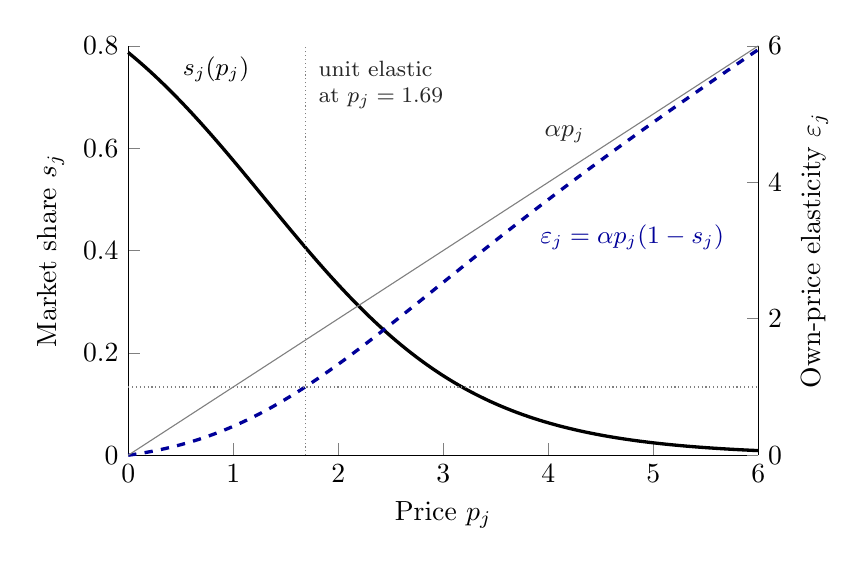
\begin{tikzpicture}
\begin{axis}[
  scale only axis, width=0.66\textwidth, height=5.2cm,
  xmin=0, xmax=6, ymin=0, ymax=0.8,
  axis y line*=left, axis x line*=bottom,
  xlabel={Price $p_j$}, ylabel={Market share $s_j$},
  ytick={0,0.2,0.4,0.6,0.8},
  yticklabel style={/pgf/number format/fixed, /pgf/number format/precision=1},
  clip=false]
  \addplot[very thick, black, samples=121, domain=0:6] {exp(2-x)/(2+exp(2-x))}
    node[pos=0.07, above right, font=\small] {$s_j(p_j)$};
  \draw[densely dotted, gray] (axis cs:1.685,0) -- (axis cs:1.685,0.8);
  \node[font=\footnotesize, anchor=north west, gray!30!black, align=left] at (axis cs:1.72,0.79)
    {unit elastic\\ at $p_j = 1.69$};
\end{axis}
\begin{axis}[
  scale only axis, width=0.66\textwidth, height=5.2cm,
  xmin=0, xmax=6, ymin=0, ymax=6,
  axis y line*=right, axis x line=none,
  ylabel={Own-price elasticity $\varepsilon_j$},
  clip=false]
  \addplot[very thick, dashed, blue!60!black, samples=121, domain=0:6] {x*(1 - exp(2-x)/(2+exp(2-x)))}
    node[pos=0.62, below right, font=\small] {$\varepsilon_j = \alpha p_j(1 - s_j)$};
  \addplot[thin, gray, domain=0:6] {x} node[pos=0.74, above left, font=\small, gray!30!black] {$\alpha p_j$};
  \addplot[densely dotted, gray, domain=0:6] {1};
\end{axis}
\end{tikzpicture}
\caption{Logit demand and its own-price elasticity. The solid curve (left axis) is the share of one product,
$s_j = \frac{e^{2 - p_j}}{2 + e^{2 - p_j}}$, holding the other options fixed, with $\alpha = 1$. The dashed
curve (right axis) is the own-price elasticity $\alpha p_j(1 - s_j)$, which approaches the line $\alpha p_j$ as
the share falls. The dotted horizontal line marks an elasticity of one.}
\label{fig:07-logit-demand}
\end{figure}

\casehead{The source of the restriction}
A consumer buys product $j$ either because $\delta_j$ is high or because her shock $\epsilon_{ij}$ is high.
When $p_j$ rises, the consumers who leave $j$ are those whose shock $\epsilon_{ij}$ was just large enough to make
$j$ their choice. Their shocks for the other products are independent of $\epsilon_{ij}$. Their second choices
therefore follow the same distribution as the first choices of the population, which is the vector of market
shares \citep[p.~523]{Nevo2000a}. \citet[p.~246]{Berry1994} stresses that the restriction comes from the i.i.d.
additive error. Whenever tastes vary only through such an error, the mean utilities $\delta_j$ determine shares
and elasticities. Two products with the same shares then have the same cross elasticity with any third product,
whatever the distribution of the error (\cref{rem:07-berry-iid} gives the argument). An independent probit has
the same problem, which led \citet{HausmanWise1978} to allow correlated errors.

The cure is correlation of utility across similar products. The nested logit (\cref{sec:07-nested}) builds the
correlation into the shock. Random coefficients (\cref{ch:blp}) generate it from heterogeneous tastes for
characteristics. Both remedies add heterogeneity across consumers. A different distribution for an
independent shock would leave the problem in place. \citet[pp.~1414--1415]{McFadden1984} adds a related point.
IIA follows from letting the utility of $j$ depend only on the attributes of $j$. If utilities may depend on the
attributes of all alternatives, the logit form can approximate any continuous choice model
(\cref{rem:06-universal}). The restriction lies in the specification of utility, and the logistic function
plays no part in it.

\casehead{Other functional forms for price}
The elasticity pattern also reflects the linearity of utility in price. Suppose utility depends on the
logarithm of price, $\delta_j = x_j\beta - \alpha\ln p_j + \xi_j$. Then $\frac{\partial \delta_j}{\partial p_j} =
-\frac{\alpha}{p_j}$ and
\begin{equation*}
  \frac{\partial s_j}{\partial p_j} = -\frac{\alpha}{p_j}\,s_j(1 - s_j), \qquad
  \varepsilon_j = \alpha(1 - s_j),
\end{equation*}
which is nearly constant across products \citep[pp.~522--523]{Nevo2000a}. \citet{BjornerstedtVerboven2016}
compare a unit-demand nested logit, linear in price, with a constant-expenditure version. In the latter, price
enters in logarithms and a buyer spends a constant fraction of income on the chosen product (eq.~(3), p.~139).
For Swedish analgesics in December 2008, their nested logit models give average brand-level own elasticities of
2.43 under constant expenditure and 8.84 under unit demand (Table~6, p.~147). The difference has large consequences
for predicted merger effects (\cref{ch:mergers}).
\citet[p.~231]{AskerNocke2021} list the paper among the ex-post evaluations of the accuracy of merger simulation.
Either way, the functional form decides how own elasticities vary across products before any data are used.

Income effects require leaving the quasi-linear form. With $u_{ij} = \alpha\ln(y_i - p_j) + x_j\beta + \xi_j +
\epsilon_{ij}$, income no longer cancels, and the marginal utility of money $\frac{\alpha}{y_i - p_j}$ varies
across consumers. Market shares become averages of logit probabilities over the income distribution of the
market. This is a random coefficients model, and its shares must be simulated (\cref{ch:blp}).

\begin{remark}[Adequacy depends on the use]\label{rem:07-adequacy}
Whether the logit is good enough cannot be judged in isolation. If a question does not hinge on the matrix of
cross elasticities, the logit may serve well. \citet{Einav2007} uses a nested logit without prices to separate
seasonal swings in the demand for movies from seasonal swings in the number and quality of releases
(\cref{sec:07-einav}). The same model would be a poor basis for merger simulation, which depends on the
cross elasticities between close substitutes.
\end{remark}

\subsection{Logit with individual data: maximum likelihood}\label{sec:07-micro-ml}

The logit began as a model of individual choice. \citet{McFadden1974} introduced the \emph{conditional
logit}, in which choice probabilities depend on attributes of the alternatives, and studied its maximum
likelihood estimator. Individual data let us interact product characteristics with consumer attributes, which
relaxes IIA across consumer types.

\casehead{The conditional logit with consumer attributes}
Suppose we observe in each market $t$ a sample $\mathcal{I}_t$ of consumers, their attributes $D_i$ (an
$R$-vector), and their choices $y_{ijt} \in \{0, 1\}$. Let
\begin{equation}\label{eq:07-micro-utility}
  u_{ijt} = \delta_{jt} + \sum_{k=1}^{K}\sum_{r=1}^{R} x_{jkt}\pi_{kr}D_{ir} + \epsilon_{ijt}, \qquad
  u_{i0t} = \epsilon_{i0t},
\end{equation}
with $\epsilon_{ijt}$ as in \cref{asm:07-logit}. The terms $\delta_{jt}$ are \emph{alternative-specific
constants}, one for each product and market. They absorb $x_{jt}\beta - \alpha p_{jt} + \xi_{jt}$ in full. The
coefficients $\pi_{kr}$ let consumers with different attributes value characteristics differently. Collect the
parameters in $\theta = (\delta, \pi)$. Write the deterministic utility as $V_{ijt} = w_{ijt}\theta$, where the
row vector $w_{ijt}$ contains a dummy for the pair $(j, t)$ and the interactions $x_{jkt}D_{ir}$, and set
$w_{i0t} = 0$. The choice probabilities and the log-likelihood are
\begin{equation}\label{eq:07-micro-ll}
  P_{ijt}(\theta) = \frac{e^{w_{ijt}\theta}}{\sum_{k=0}^{J_t} e^{w_{ikt}\theta}}, \qquad
  \ell(\theta) = \sum_{t=1}^{T}\sum_{i \in \mathcal{I}_t}\sum_{j=0}^{J_t} y_{ijt}\ln P_{ijt}(\theta) .
\end{equation}

\begin{proposition}[Global concavity]\label{prop:07-ml-concave}
The log-likelihood in \eqref{eq:07-micro-ll} is concave in $\theta$. It is strictly concave if the matrix that
stacks the rows $w_{ijt}$, over all sampled consumers $i$, all $j \in \mathcal{J}_t$ and all $t$, has full
column rank. A stationary point of $\ell$ is then its unique global maximum.
\end{proposition}

\begin{proof}
Fix a consumer $i$ in market $t$ and drop the index $t$. Since $\sum_j y_{ij} = 1$, her contribution to the
log-likelihood is
\begin{equation*}
  \ell_i(\theta) = \sum_j y_{ij}w_{ij}\theta - \ln\sum_k e^{w_{ik}\theta} .
\end{equation*}
The first term is linear in $\theta$. Differentiating once,
\begin{equation*}
  \frac{\partial \ell_i}{\partial \theta}
  = \sum_j y_{ij}w_{ij}^\T - \sum_k P_{ik}w_{ik}^\T
  = \sum_j (y_{ij} - P_{ij})\,w_{ij}^\T .
\end{equation*}
Let $\bar w_i = \sum_k P_{ik}w_{ik}$ be the probability-weighted mean of the rows. The probabilities satisfy
$\frac{\partial P_{ik}}{\partial \theta^\T} = P_{ik}(w_{ik} - \bar w_i)$. Differentiating a second time,
\begin{equation*}
  \frac{\partial^2 \ell_i}{\partial \theta\,\partial \theta^\T}
  = -\sum_k P_{ik}\,w_{ik}^\T(w_{ik} - \bar w_i)
  = -\sum_k P_{ik}\,(w_{ik} - \bar w_i)^\T(w_{ik} - \bar w_i),
\end{equation*}
where the second equality subtracts $\bar w_i^\T\sum_k P_{ik}(w_{ik} - \bar w_i) = 0$. For any vector $v$,
\begin{equation*}
  v^\T\,\frac{\partial^2 \ell_i}{\partial \theta\,\partial \theta^\T}\,v
  = -\sum_k P_{ik}\big[(w_{ik} - \bar w_i)v\big]^2 \le 0 .
\end{equation*}
The right side is minus the variance of $w_{ik}v$ when $k$ is drawn with probabilities $P_{ik}$. Summing over
consumers shows that the Hessian of $\ell$ is negative semidefinite at every $\theta$, so $\ell$ is concave.

For strict concavity, suppose that $v^\T\nabla^2\ell(\theta)v = 0$. Every $P_{ik}$ is positive, so
$(w_{ik} - \bar w_i)v = 0$ for all $i$ and $k$. Then $w_{ik}v$ takes the same value for every option $k$ of
consumer $i$, and that value is $w_{i0}v = 0$. Hence $w_{ijt}v = 0$ for every row of the stacked matrix, and
the rank condition gives $v = 0$. A strictly concave function has at most one maximizer, and any stationary
point is that maximizer.
\end{proof}

\citet{McFadden1974} established this property, and \citet[p.~1413]{McFadden1984} restates it: barring linear
dependence of the explanatory variables, any stationary value is a global maximum. \Cref{eq:06-hessian}
derives the same Hessian in the notation of \cref{ch:discrete}. Concavity has practical value. Newton's method
with a line search, such as step-halving, converges to the maximum from any starting value. The estimate
therefore does not depend on where the search begins. Undamped Newton steps can still overshoot from poor
starting values. A maximum can
fail to exist when some combination of the regressors predicts the observed choices perfectly, as with
separation in a binary logit.

\casehead{Constants and shares}
The first-order condition for the constant $\delta_{jt}$ reads
\begin{equation}\label{eq:07-micro-foc}
  \frac{\partial \ell}{\partial \delta_{jt}} = \sum_{i \in \mathcal{I}_t}\big(y_{ijt} - P_{ijt}(\hat\theta)\big) = 0,
\end{equation}
so the average predicted probability of $j$ equals its sample share $\hat s_{jt}$. Without interactions
($\pi = 0$), every consumer in market $t$ has $P_{ijt} = \frac{e^{\delta_{jt}}}{1 + \sum_k e^{\delta_{kt}}}$, and
\eqref{eq:07-micro-foc} gives $\hat\delta_{jt} = \ln\hat s_{jt} - \ln\hat s_{0t}$. The maximum likelihood
estimates of the constants are the logit inversion of the sample shares, which \cref{sec:07-inversion-logit}
derives for market data.

\casehead{Micro data do not remove the need for instruments}
The constants absorb $\xi_{jt}$, so the likelihood in \eqref{eq:07-micro-ll} has no endogeneity problem. The
price coefficient, however, cannot be estimated from it. All consumers in a market face the same price, so
$p_{jt}$ is collinear with the dummy for $(j, t)$. The coefficients $\beta$ and $\alpha$ come from a second
step that regresses the estimated constants on characteristics and prices,
\begin{equation}\label{eq:07-micro-second}
  \hat\delta_{jt} = x_{jt}\beta - \alpha p_{jt} + \xi_{jt} + (\hat\delta_{jt} - \delta_{jt}) .
\end{equation}
This step compares products and markets. There $p_{jt}$ is correlated with $\xi_{jt}$ for the reasons given in
\cref{sec:07-endogeneity}, so the second step needs instruments, exactly as with market data
\citep[p.~259]{Berry1994}. Micro data reveal how tastes differ across consumers within a market, including
interactions of price with income. The average response to price still requires exogenous variation in
prices. \Cref{sec:08-micro-twostep} develops the two-step estimator with random coefficients, and \cref{ch:blp}
discusses \citet{Goldberg1995} and \citet*{BerryLevinsohnPakes2004}.

\casehead{Testing IIA}
IIA has a testable implication. Let $D$ be a subset of the full choice set $C$. If the logit is correct, the
probability of choosing $j$ given that the choice lies in $D$ is the logit $\frac{e^{V_{ij}}}{\sum_{k \in D}
e^{V_{ik}}}$, with the same parameters. We can therefore estimate the model on the consumers who chose an
alternative in $D$, treating $D$ as their choice set. This gives a consistent but inefficient estimator
$\hat\beta_D$ of the parameters that choices within $D$ identify. The full-sample estimator $\hat\beta_C$ is
consistent and efficient. If IIA fails,
the two estimators generally converge to different limits. Following the principle of \citet{Hausman1978},
the variance of the difference under the null is the difference of the variances, $\hat V_D - \hat V_C$. The
statistic
\begin{equation}\label{eq:07-hm-test}
  S = (\hat\beta_D - \hat\beta_C)^\T\,(\hat V_D - \hat V_C)^{-}\,(\hat\beta_D - \hat\beta_C),
\end{equation}
where $^{-}$ denotes a generalized inverse when the difference of the variances is singular. The statistic
is asymptotically chi-squared with degrees of freedom equal to the rank of $\hat V_D - \hat V_C$
\citep[pp.~1417--1418]{McFadden1984}. \citet{HausmanMcFadden1984} develop the test. McFadden cautions that it
is an omnibus test, which may reject because of misspecifications other than IIA. He adds that it has little
power unless the departures from the logit are substantial.

\citet[Section~3.11]{McFadden1984} applies the test to the housing status of 159 single elderly men in the
Albany-Schenectady-Troy (New York) metropolitan area, from the 1977 U.S. Annual Housing Survey. The
alternatives are to own (73 cases), to rent as a non-head of household (38 cases) and to rent as head (48
cases). Two variables measure prices: the out-of-pocket cost of each alternative (\textit{OPCOST}) and the
expected net return on equity in owned units (\textit{RETURN}). Income enters through interactions with dummies
for owning (\textit{YOWN}) and for non-headship (\textit{YNH}). \Cref{tab:07-mcfadden-housing} reproduces the logit
estimates. Deleting the owner alternative gives $S_{\text{own}} = 22.4$. McFadden compares it with the
chi-squared distribution with three degrees of freedom and rejects IIA at the 0.001 level. Deleting the
renter-head alternative gives $S_{\text{head}} = 1.7$, which does not reject. He concludes that the logit
should be rejected.

A nested logit that groups the two rental options confirms the verdict. Its \emph{inclusive value coefficient}
multiplies the logarithm of the summed exponentiated utilities of the two rental options, and the logit sets it
to one. In the notation of \cref{sec:07-nested} it equals $1 - \sigma$. McFadden first tests the logit against
this tree with the Lagrange multiplier statistic of his equation (3.59), which needs only the logit estimates
(pp.~1427--1428). It is asymptotically chi-squared with one degree of freedom, and its value of 15.73 rejects the
logit at the 0.001 level (p.~1431).

Panel B of \cref{tab:07-mcfadden-housing} reports the full maximum likelihood estimates of the nested logit
(Table 3.3). The inclusive value coefficient is 0.179 (standard error 0.109), so $\sigma = 1 - 0.179 = 0.821$.
\textit{OPCOST}, \textit{RETURN} and \textit{YNH} keep their logit signs, while \textit{YOWN}, insignificant in
both models, turns positive. \textit{OPCOST} and \textit{YNH} remain significant, and \textit{RETURN} is
significant at the 10 percent level only. The Wald statistic for the restriction that the
coefficient equals one is 56.77, which rejects at the 0.001 level. The likelihood ratio statistic is
\begin{equation*}
  LR = 2\,\big[-10.79 - (-15.91)\big] = 10.24 ,
\end{equation*}
which rejects at the 0.005 level but not at the 0.001 level. The three statistics satisfy $LR < LM < W$.
McFadden reads their spread as a warning that first-order asymptotics may be inaccurate in a sample of 159
(p.~1431). Panel D shows what IIA imposes. In the logit, the elasticities of owning and of renting as head with
respect to the cost of renting as non-head are both 1.06. The nested logit gives 5.15 for the close substitute
and 0.54 for owning.

\begin{table}[htbp]
\centering
\caption{Logit and nested logit models of housing status in \citet{McFadden1984}}
\label{tab:07-mcfadden-housing}
\begin{tabular}{@{}lccc@{}}
\toprule
\multicolumn{4}{@{}l}{\textit{Panel A. Logit estimates (Table 3.2)}} \\
Variable & Estimate & Standard error & $t$-statistic \\
\midrule
\textit{OPCOST} & $-4.544$ & 1.011 & $-4.50$ \\
\textit{RETURN} & 2.506 & 0.747 & 3.35 \\
\textit{YOWN} & $-0.055$ & 0.074 & $-0.73$ \\
\textit{YNH} & $-0.838$ & 0.202 & $-4.16$ \\
\addlinespace
Log-likelihood & \multicolumn{3}{l}{$-15.91$ (sample size 159)} \\
\midrule
\multicolumn{4}{@{}l}{\textit{Panel B. Nested logit estimates, rental options in one nest (Table 3.3)}} \\
Variable & Estimate & Standard error & $t$-statistic \\
\midrule
\textit{OPCOST} & $-2.334$ & 0.622 & $-3.75$ \\
\textit{RETURN} & 0.922 & 0.479 & 1.93 \\
\textit{YOWN} & 0.034 & 0.064 & 0.53 \\
\textit{YNH} & $-0.438$ & 0.121 & $-3.62$ \\
Inclusive value coefficient & 0.179 & 0.109 & 1.64 \\
\addlinespace
Log-likelihood & \multicolumn{3}{l}{$-10.79$ (sample size 159)} \\
\midrule
\multicolumn{4}{@{}l}{\textit{Panel C. Specification tests of the logit (pp.~1430--1431)}} \\
Owner alternative deleted & \multicolumn{3}{l}{$S_{\text{own}} = 22.4$ (3 degrees of freedom)} \\
Renter-head alternative deleted & \multicolumn{3}{l}{$S_{\text{head}} = 1.7$ (3 degrees of freedom)} \\
Inclusive value coefficient $= 1$ & \multicolumn{3}{l}{$LM = 15.73$, $W = 56.77$, $LR = 10.24$ (1 degree of freedom)} \\
\midrule
\multicolumn{4}{@{}l}{\textit{Panel D. Elasticities with respect to the rental non-head \textit{OPCOST} (Table 3.4)}} \\
 & Own & Rent, non-head & Rent, head \\
\midrule
Logit & 1.06 & $-3.35$ & 1.06 \\
Nested logit & 0.54 & $-7.48$ & 5.15 \\
\bottomrule
\end{tabular}

\vspace{4pt}
\begin{minipage}{0.86\textwidth}
\footnotesize Notes: 159 single elderly men, 1977 U.S. Annual Housing Survey, Albany-Schenectady-Troy.
Alternatives: own (73), rent as non-head (38), rent as head (48). Costs and returns in thousands of 1977
dollars. Panel B: full maximum likelihood, with the units within each cluster treated as homogeneous. Its
$t$-statistic for the inclusive value coefficient tests a value of zero. Panel C: $S$ is the Hausman-McFadden
statistic of \eqref{eq:07-hm-test}, and $LM$, $W$ and $LR$ test the logit against the nested logit of Panel B.
Panel D: elasticities at sample means. Source: \citet[Tables 3.2 to 3.4 and pp.~1430--1431]{McFadden1984}.
\end{minipage}
\end{table}

\casehead{Sampling alternatives and choice-based samples}
IIA also simplifies estimation. Under IIA, the model can be estimated on a random subset of the alternatives
\citep[Section~3.6]{McFadden1984}. This helps when the choice set is very large, such as the stock of dwellings
in a housing market. When the sample is stratified on the chosen alternative, as in surveys of the buyers of
particular products, the weighted estimator of \citet{ManskiLerman1977} restores consistency in any choice
model \citep[Section~4.4]{McFadden1984}. The logit allows a simpler route. Selection rates that depend only on
the chosen alternative enter its probabilities as shifts in the alternative-specific constants, so the
conditional likelihood of the sample keeps the logit form \citep[eq.~4.15]{McFadden1984}.

\casehead{McFadden's survey in context}
\citet{McFadden1984} organizes the econometrics of discrete choice around the random utility model and
maximum likelihood. He compares three families of functional forms, built on the work of Luce (logit),
Thurstone (probit) and Tversky (elimination models). In his verdict the multinomial logit ``scores well on
simplicity and computation, but poorly on flexibility'' (p.~1410). The generalized extreme value family of
\citet{McFadden1978} keeps closed forms while allowing similarity among alternatives (Sections~3.9 and 3.10), and
\cref{sec:07-nested} uses it. McFadden also finds the logit ``relatively robust, as measured by goodness of fit
or prediction accuracy, in many cases where the IIA property is theoretically implausible'' (p.~1414). That
robustness helps explain why the logit remains the first model that applied researchers estimate.

\section{The Berry inversion}\label{sec:07-inversion}

Industrial organization economists rarely observe individual choices. They usually observe prices,
characteristics and quantities for many products in many markets. \citet{Berry1994} showed how to estimate
discrete choice demand from such data when an unobserved characteristic is correlated with price. This section
explains the problem he solved, derives his inversion for the logit, proves that the inversion exists in a
general class of models, and discusses the data it requires.

\subsection{The estimation problem with aggregate data}\label{sec:07-inversion-problem}

Suppose we observe, for markets $t = 1, \dots, T$, the shares $s_{jt} = \frac{q_{jt}}{M_t}$, prices $p_{jt}$,
characteristics $x_{jt}$ and cost shifters $w_{jt}$. The model says that observed shares equal predicted shares,
\begin{equation}\label{eq:07-share-equation}
  s_{jt} = s_j(x_t, p_t, \xi_t; \theta), \qquad j \in \mathcal{J}_t,
\end{equation}
where $x_t$, $p_t$ and $\xi_t$ stack the characteristics, prices and unobserved characteristics of all products
in market $t$ \citep[eq.~10]{Berry1994}. Prices are correlated with $\xi_t$. With homogeneous goods, an
additive demand error and instruments for price solve this problem. Here the error enters
\eqref{eq:07-share-equation} nonlinearly, through every product's share, ``thus frustrating the application of
traditional instrumental variables methods'' \citep[p.~248]{Berry1994}. To see why, consider nonlinear least
squares on $s_{jt} = s_j(x_t, p_t, 0; \theta) + e_{jt}$. The composite error $e_{jt} = s_j(x_t, p_t, \xi_t;
\theta) - s_j(x_t, p_t, 0; \theta)$ is a nonlinear function of $\xi_t$ and of the prices. Its mean given the
instruments is generally not zero, even when $\E[\xi_{jt} \mid z_t] = 0$, because the conditional mean of a
nonlinear function differs from the function of the conditional mean. No choice of instruments restores a valid
moment condition at the true parameters.

Before 1994, applied work took one of three routes. The first worked in product space, with the
constant-elasticity system $\ln q_j = a_j + \sum_k \varepsilon_{jk}\ln p_k + e_j$ \citep[eq.~1]{Berry1994}.
The error is additive, so instrumental variables apply. But $J$ goods require $J^2$ elasticities, and the roughly
100 automobiles in \citet{Bresnahan1987} imply almost 10,000 of them \citep[p.~244]{Berry1994}
(\cref{ch:aids}). The second estimated discrete choice models while ignoring unobserved characteristics. Prices
then absorb the effect of omitted quality. In \citeauthor{Trajtenberg1989}'s (\citeyear{Trajtenberg1989})
study of CT scanners, price sometimes appears to raise demand, an anomaly he attributes to unobserved quality
\citep[p.~243]{Berry1994}. The third, used by \citet{Bresnahan1987}, replaced unobserved characteristics with
measurement error in prices and quantities (\cref{ch:discrete}).

\citet[Section~7]{Berry1994} also explains why three tempting shortcuts fail. The first treats each $\xi_j$ as
a fixed effect to be estimated with $\beta$ and $\alpha$. Mean utility is $\delta_j = x_j\beta - \alpha p_j +
\xi_j$, and any combination of $(\xi_1, \dots, \xi_J, \beta, \alpha)$ that produces the same $\delta$ predicts
the same choices. The vector $\xi$ is therefore not identified separately from the coefficients on
product-level variables. The logic is that of grouped data: a group mean cannot be estimated together with the
coefficients of variables that do not vary within the group. With panel data, product fixed effects absorb only
the time-invariant part of $\xi_{jt}$ (\cref{sec:07-fixed-effects}).

The second shortcut integrates $\xi$ out of the share function while holding prices fixed. Optimal prices
respond to $\xi$, so the distribution of $\xi_t$ conditional on $p_t$ differs from its unconditional
distribution $\Phi$. Formally,
\begin{equation*}
  \E[s_{jt} \mid x_t, p_t] = \int s_j(x_t, p_t, \xi; \theta)\,\dd\Phi(\xi \mid x_t, p_t)
  \ne \int s_j(x_t, p_t, \xi; \theta)\,\dd\Phi(\xi),
\end{equation*}
and matching observed shares to the right side gives inconsistent estimates. Berry notes that the
price-setting model is inconsistent with any assumption of an exogenous distribution of $\xi$ conditional on
$x$ and $p$ \citep[p.~256]{Berry1994}.

The third shortcut solves for the reduced form. Suppose equilibrium is unique, so that prices $p(z, \xi,
\omega, \theta)$ and quantities $q(z, \xi, \omega, \theta)$ are functions of the observed data $z$, the demand
and cost unobservables $(\xi, \omega)$ and the parameters. Integrating over a distribution $\Phi(\cdot \mid z,
\theta_u)$ of the unobservables gives expected prices and quantities,
\begin{align*}
  \bar p(z, \theta, \theta_u) &= \int p(z, \xi, \omega, \theta)\,\Phi\big(\dd(\xi, \omega) \mid z, \theta_u\big),\\
  \bar q(z, \theta, \theta_u) &= \int q(z, \xi, \omega, \theta)\,\Phi\big(\dd(\xi, \omega) \mid z, \theta_u\big),
\end{align*}
and nonlinear least squares can fit $p = \bar p + v$ and $q = \bar q + e$ \citep[eqs.~34 and
35]{Berry1994}. \citet{Bresnahan1987} and \citet{Berry1990} took this route. It has two problems. The integrals
are over implicitly defined functions, which are costly to evaluate at every trial parameter. More seriously,
they require a unique equilibrium for almost all values of the unobservables, and existence at particular values
is not enough. Uniqueness is hard to establish in this class of models, although \citet{CaplinNalebuff1991}
prove it for the logit and the vertical model \citep[p.~257]{Berry1994}. The reduced form has one advantage.
It is linear in observed prices and quantities, so it tolerates measurement error in them.

The key idea of \citet{Berry1994} is to write $\delta(s)$ instead of $s(\delta)$. Suppose the distribution of
the consumer-specific terms is known, so that shares depend on the data only through the mean utilities,
$s_t = s(\delta_t)$. If this system can be inverted at the observed shares, the structural error enters
linearly:
\begin{equation}\label{eq:07-berry-linear}
  \delta_{jt}(s_t) = x_{jt}\beta - \alpha p_{jt} + \xi_{jt}
\end{equation}
\citep[eq.~12]{Berry1994}. Standard instrumental variables then apply, with $\delta_{jt}(s_t)$ as the dependent
variable and $\xi_{jt}$ as the error. Berry stresses that the transformation of the data is unimportant.
Apart from the computation, he writes, the approach ``is little different than'' regressions that use ``some
other transformation of the observed data (e.g., logarithms) as a dependent variable'' (p.~249). Mean
utilities play the role that quantities play in a homogeneous-goods demand regression. Demand estimation then
requires neither a parametric distribution for $\xi$ nor a model of how prices are set (p.~249).

\subsection{The logit inversion}\label{sec:07-inversion-logit}

In the logit the inverse has a closed form. Divide the share of product $j$ in \eqref{eq:07-logit-share} by the
outside share. The inclusive sum cancels:
\begin{equation*}
  \frac{s_{jt}}{s_{0t}} = \frac{\frac{e^{\delta_{jt}}}{\Lambda_t}}{\frac{1}{\Lambda_t}} = e^{\delta_{jt}},
  \qquad \Lambda_t = 1 + \sum_{k \in \mathcal{J}_t} e^{\delta_{kt}} .
\end{equation*}
Taking logarithms gives $\delta_{jt} = \ln s_{jt} - \ln s_{0t}$. Substituting the specification of mean utility
yields the estimating equation
\begin{equation}\label{eq:07-logit-inversion}
  \ln s_{jt} - \ln s_{0t} = x_{jt}\beta - \alpha p_{jt} + \xi_{jt}, \qquad
  s_{0t} = 1 - \sum_{j \in \mathcal{J}_t} s_{jt}
\end{equation}
\citep[eq.~14]{Berry1994}. \citet[eqs.~6.4 and 6.5]{BerryLevinsohnPakes1995} write the implied demand
unobservable as $\xi_{jt} = \ln s_{jt} - \ln s_{0t} - x_{jt}\beta + \alpha p_{jt}$.

Equation \eqref{eq:07-logit-inversion} is a linear regression with a known dependent variable and a structural
error. Prices are endogenous, so it is estimated by two-stage least squares or the linear generalized method of moments with instruments for
price (\cref{sec:07-endogeneity}). The linear form is the main reason the logit is used so much. Estimation is
cheap, so the logit is a natural first look at any data set before richer models are tried. Three features of
the equation deserve emphasis.

First, the inversion uses the observed shares, so the model fits them exactly. Every discrepancy between data and
model is attributed to $\xi_{jt}$ \citep[p.~533]{Nevo2000a}. Second, the outside share requires the market size
$M_t$, which \cref{sec:07-market-size} discusses. Third, each market is one observation of a system of $J_t$
equations. With many independent markets, the errors may be correlated arbitrarily within a market
\citep[p.~250]{Berry1994}. With a single market, the demand parameters can still be estimated from many
products if the $\xi_j$ are independent across products. Prices are then still correlated across products
through the first-order conditions, which raises issues of dependence (footnote~6).

\subsection{Invertibility in general}\label{sec:07-invertibility}

The logit is unusual in having an explicit inverse. For other models, we need to know that the system $s =
s(\delta)$ has exactly one solution for every observed share vector. \citet[Appendix]{Berry1994} proves this
for a broad class of models. Fix a market and drop its index. Let utility be $u_{ij} = \delta_j + \nu_{ij}$ for
$j = 0, 1, \dots, J$, where the vector $\nu_i = (\nu_{i0}, \dots, \nu_{iJ})$ has a distribution that does not
depend on $\delta$. The logit is the case $\nu_{ij} = \epsilon_{ij}$. The random coefficients logit of
\cref{ch:blp} is the case $\nu_{ij} = \mu_{ij} + \epsilon_{ij}$. Shares are
\begin{equation}\label{eq:07-general-share}
  s_j(\delta_0, \delta_1, \dots, \delta_J) = \Pr\big(\delta_j + \nu_{ij} > \delta_k + \nu_{ik}
  \text{ for all } k \ne j\big),
\end{equation}
viewed as functions of all $J + 1$ mean utilities and evaluated at $\delta_0 = 0$. Let $H_j(\delta_j) =
\Pr(\delta_j + \nu_{ij} > \nu_{i0})$ be the share that $j$ would have if only $j$ and the outside good were
available.

\begin{proposition}[Invertibility of market shares]\label{prop:07-invertibility}
Suppose that
\begin{enumerate}[label=(\alph*)]
  \item The share functions are continuously differentiable in $(\delta_0, \dots, \delta_J)$.
  \item The derivatives satisfy $\frac{\partial s_j}{\partial \delta_j} > 0$ and $\frac{\partial s_j}{\partial
  \delta_k} < 0$ for every $k \ne j$, including $k = 0$.
  \item Each $H_j$ is continuous and strictly increasing, with limits 0 and 1 as $\delta_j \to -\infty$ and
  $\delta_j \to \infty$.
\end{enumerate}
Let $s^{\mathrm{obs}} = (s^{\mathrm{obs}}_1, \dots, s^{\mathrm{obs}}_J)$ satisfy $s^{\mathrm{obs}}_j > 0$ for
every $j$ and $s^{\mathrm{obs}}_0 = 1 - \sum_j s^{\mathrm{obs}}_j > 0$. Then exactly one $\delta \in \R^J$
satisfies $s_j(0, \delta) = s^{\mathrm{obs}}_j$ for $j = 1, \dots, J$.
\end{proposition}

A density of $\nu_i$ that is strictly positive and continuous on $\R^{J+1}$ is sufficient for the conditions
\citep[p.~260]{Berry1994}. \Citet*{BerryGandhiHaile2013} give a general version, discussed after the proof.

\begin{proof}
We follow \citet[pp.~260--261]{Berry1994} and write $s_j(\delta)$ for $s_j(0, \delta)$.

\emph{Step 1: the element-by-element inverse.} Fix $j$ and the other inside mean utilities $\delta_{-j}$. As
$\delta_j$ rises from $-\infty$ to $\infty$, $s_j$ rises strictly by (b), from 0 to 1, because the shocks are
finite with probability one. So exactly one value $r_j(\delta_{-j})$ solves
\begin{equation}\label{eq:07-elementwise}
  s_j\big(\delta_1, \dots, \delta_{j-1}, r_j(\delta_{-j}), \delta_{j+1}, \dots, \delta_J\big) = s^{\mathrm{obs}}_j .
\end{equation}
By the implicit function theorem, $r_j$ is continuously differentiable with
\begin{equation}\label{eq:07-r-derivative}
  \frac{\partial r_j}{\partial \delta_k} = -\frac{\frac{\partial s_j}{\partial \delta_k}}{\frac{\partial s_j}
  {\partial \delta_j}} > 0, \qquad k \ne j,\ k \ge 1 .
\end{equation}
Let $r = (r_1, \dots, r_J)$ and treat $r_j$ as a function of the whole vector $\delta$ that ignores
$\delta_j$. If $s(\delta) = s^{\mathrm{obs}}$, then each $\delta_j$ solves \eqref{eq:07-elementwise}, so
$\delta_j = r_j(\delta)$. Conversely, $\delta = r(\delta)$ implies $s(\delta) = s^{\mathrm{obs}}$. The
inverse problem is therefore the fixed-point problem $\delta = r(\delta)$.

\emph{Step 2: a lower bound.} Adding products can only lower the share of $j$, since the event that $j$ beats
every option is contained in the event that $j$ beats the outside good. Hence $s_j(\delta) \le
H_j(\delta_j)$ for every $\delta$. At $\delta_j = r_j(\delta)$ this gives $s^{\mathrm{obs}}_j \le
H_j(r_j(\delta))$, so
\begin{equation*}
  r_j(\delta) \ge H_j^{-1}(s^{\mathrm{obs}}_j) \ge \underline\delta \equiv \min_k H_k^{-1}(s^{\mathrm{obs}}_k)
  \quad \text{for every } \delta .
\end{equation*}

\emph{Step 3: an upper bound (Berry's lemma).} Let $\bar\delta_j = H_j^{-1}(1 - s^{\mathrm{obs}}_0)$, the mean
utility at which $j$ alone would leave the outside good with its observed share. Choose $\bar\delta >
\max_j \bar\delta_j$. We claim that if $\delta_j \ge \bar\delta$ for some $j$, then $r_k(\delta) < \delta_k$
for some $k$. Indeed, the event that the outside good beats every option is contained in the event that it
beats $j$, so
\begin{equation*}
  s_0(\delta) \le 1 - H_j(\delta_j) < 1 - H_j(\bar\delta_j) = s^{\mathrm{obs}}_0 ,
\end{equation*}
where the strict inequality uses $\delta_j > \bar\delta_j$ and (c). The inside shares at $\delta$ therefore sum to
more than $\sum_k s^{\mathrm{obs}}_k$, so some product $k$ has $s_k(\delta) > s^{\mathrm{obs}}_k$. Since $s_k$
rises strictly in $\delta_k$, matching $s^{\mathrm{obs}}_k$ requires a lower value, that is, $r_k(\delta) <
\delta_k$. Note also that $\bar\delta > \underline\delta$, because $1 - s^{\mathrm{obs}}_0 \ge
s^{\mathrm{obs}}_j$ implies $\bar\delta_j \ge H_j^{-1}(s^{\mathrm{obs}}_j)$.

\emph{Step 4: existence.} Define the truncated map $\bar r_j(\delta) = \min\{r_j(\delta), \bar\delta\}$. By Steps 1
and 2, $\bar r$ is continuous and maps $\R^J$ into the box $B = [\underline\delta, \bar\delta]^J$. Brouwer's
fixed-point theorem applied to $\bar r$ on the compact convex set $B$ gives a point $\delta^* \in B$ with
$\delta^* = \bar r(\delta^*)$. Suppose some component satisfies $\delta^*_j = \bar\delta$. By Step 3 there is a
$k$ with $r_k(\delta^*) < \delta^*_k$, and then $\bar r_k(\delta^*) \le r_k(\delta^*) < \delta^*_k$, which
contradicts $\delta^* = \bar r(\delta^*)$. Hence every $\delta^*_j < \bar\delta$. Then $\min\{r_j(\delta^*),
\bar\delta\} = \delta^*_j < \bar\delta$ forces $r_j(\delta^*) = \delta^*_j$. So $\delta^*$ is a fixed point of $r$,
and $s(\delta^*) = s^{\mathrm{obs}}$.

\emph{Step 5: uniqueness.} Adding the same constant to all of $(\delta_0, \delta_1, \dots, \delta_J)$ leaves every
share unchanged. Differentiating $s_j(\delta_0 + c, \dots, \delta_J + c)$ with respect to $c$ at $c = 0$ gives
\begin{equation*}
  \sum_{k=0}^{J}\frac{\partial s_j}{\partial \delta_k} = 0
  \quad\Longrightarrow\quad
  \frac{\partial s_j}{\partial \delta_j} + \sum_{k \ge 1,\, k \ne j}\frac{\partial s_j}{\partial \delta_k}
  = -\frac{\partial s_j}{\partial \delta_0} > 0 .
\end{equation*}
Divide by $\frac{\partial s_j}{\partial \delta_j} > 0$ and use \eqref{eq:07-r-derivative}:
\begin{equation}\label{eq:07-rowsum}
  \sum_{k \ge 1,\, k \ne j}\frac{\partial r_j}{\partial \delta_k}
  = 1 + \frac{\frac{\partial s_j}{\partial \delta_0}}{\frac{\partial s_j}{\partial \delta_j}} < 1 .
\end{equation}
This is the diagonal dominance condition $\sum_{k \ge 1, k \ne j}|\frac{\partial s_j}{\partial \delta_k}| <
\frac{\partial s_j}{\partial \delta_j}$ of \citet[eq.~A2]{Berry1994}. Now suppose $\delta \ne \delta'$ are two
fixed points of $r$, and let $\|\cdot\|$ denote the maximum norm. For each $j$, the mean value theorem applied
to $r_j$ on the segment between $\delta'$ and $\delta$ gives a point $\tilde\delta$ on that segment with
\begin{equation*}
  |\delta_j - \delta'_j| = |r_j(\delta) - r_j(\delta')|
  = \Big|\sum_{k \ne j}\frac{\partial r_j(\tilde\delta)}{\partial \delta_k}(\delta_k - \delta'_k)\Big|
  \le \Big(\sum_{k \ne j}\frac{\partial r_j(\tilde\delta)}{\partial \delta_k}\Big)\|\delta - \delta'\|
  < \|\delta - \delta'\| .
\end{equation*}
Choosing $j$ with $|\delta_j - \delta'_j| = \|\delta - \delta'\|$ yields $\|\delta - \delta'\| < \|\delta -
\delta'\|$, a contradiction. The fixed point is unique.
\end{proof}

The logit satisfies the conditions. With a general $\delta_0$, $s_j = \frac{e^{\delta_j}}{e^{\delta_0} +
\sum_k e^{\delta_k}}$, so $\frac{\partial s_j}{\partial \delta_0} = -s_j s_0$. By \cref{prop:07-logit-derivs},
\begin{equation*}
  \sum_{k \ge 1}\frac{\partial s_j}{\partial \delta_k} = s_j(1 - s_j) - s_j\sum_{k \ge 1,\, k \ne j}s_k
  = s_j\Big(1 - \sum_{k \ge 1}s_k\Big) = s_j s_0 = -\frac{\partial s_j}{\partial \delta_0},
\end{equation*}
and the row sum in \eqref{eq:07-rowsum} equals $\sum_{k \ge 1,\, k \ne j}\frac{s_k}{1 - s_j} = 1 -
\frac{s_0}{1 - s_j} < 1$. Two-option shares are $H_j(\delta_j) = \frac{e^{\delta_j}}{1 + e^{\delta_j}}$, which satisfy (c).

\begin{remark}[A diversion reading of uniqueness]\label{rem:07-diversion-uniqueness}
In an additive random utility model the matrix $\frac{\partial s}{\partial \delta^\T}$ is symmetric, because it
is the Hessian of the expected maximum utility (\cref{thm:06-wdz}). Hence
\begin{equation*}
  \frac{\partial r_j}{\partial \delta_k}
  = -\frac{\frac{\partial s_j}{\partial \delta_k}}{\frac{\partial s_j}{\partial \delta_j}}
  = -\frac{\frac{\partial s_k}{\partial \delta_j}}{\frac{\partial s_j}{\partial \delta_j}},
\end{equation*}
which is the diversion ratio from $j$ to $k$ after a fall in $\delta_j$. The row sum \eqref{eq:07-rowsum} is one minus the
diversion ratio from $j$ to the outside good. Uniqueness thus rests on every product losing some of its
customers to the outside good. When price enters utility only through $\delta_j$, as in the logit, these are
the price diversion ratios of \eqref{eq:07-logit-diversion}, and the row sum is $1 - D_{j0}$.
\end{remark}

Three further remarks place the result. First, Berry's argument establishes existence through Brouwer's
theorem, which gives no algorithm. \citet[Appendix~I]{BerryLevinsohnPakes1995} show that the map $\delta \mapsto
\delta + \ln s^{\mathrm{obs}} - \ln s(\delta)$ is a contraction for the random coefficients logit, which both
proves invertibility and computes the inverse. \Cref{thm:08-berry94} develops that route, and
\cref{rem:08-berry-proof} compares the two proofs. Second, the proposition requires every observed share to be
positive. A product with zero observed sales has no finite mean utility, a problem taken up in
\cref{sec:07-market-size}. Third, the proof uses neither the logit form nor any property of the pricing
equilibrium. Demand estimation based on the inversion therefore does not rely on a unique equilibrium, in
contrast with the reduced-form approach \citep[p.~243]{Berry1994}.

\citet*{BerryGandhiHaile2013} weaken condition (b) to \emph{connected substitutes}. Let $s_j(\delta, p)$
denote the share function (Berry and Haile write $\sigma_j$). Goods $0, 1, \dots, J$ are connected substitutes in
$\delta$ if two conditions hold. First, each share $s_k$ is nonincreasing in $\delta_j$ for every $j \ge 1$ and
$k \ne j$. Second, for every nonempty set $\mathcal{K}$ of inside goods there are $k \in \mathcal{K}$ and $l \notin
\mathcal{K}$ (possibly $l = 0$) such that $s_l$ is strictly decreasing in $\delta_k$ \citep[Definition~1,
p.~1759]{BerryHaile2014}. Under this condition, and an index restriction on how $\xi_j$ enters, there is at most
one $\delta$ that rationalizes any interior share vector \citep[Lemma~1, p.~1760]{BerryHaile2014}. The vertical
model shows why the weaker condition matters. In it, $\frac{\partial s_j}{\partial \delta_k} = 0$ for products
that are not neighbors in price, so condition (b) fails. Yet the chain of neighbors links every inside good to
the outside good, the shares are connected substitutes, and the inverse exists in closed form
(\cref{prop:06-vinversion}).

\subsection{Other analytic inversions}\label{sec:07-inversion-examples}

A few other models share the logit's explicit inverse. In the nested logit with nesting parameter $\sigma$ and
within-nest share $s_{j \mid g}$,
\begin{equation}\label{eq:07-nl-inversion-preview}
  \ln s_{jt} - \ln s_{0t} = \delta_{jt} + \sigma\ln s_{j \mid g, t}
\end{equation}
\citep[eq.~27]{Berry1994}. \Cref{prop:07-nl-inversion} derives it, and \eqref{eq:07-nl-regression} is the
resulting estimating equation. The within-nest share depends on $\xi_{jt}$, so it is a second endogenous
regressor. In the vertical model with $u_{ij} = \delta_j - \nu_i p_j$ and products ordered by price, the
inverse is recursive:
\begin{equation*}
  \delta_j = \delta_{j-1} + (p_j - p_{j-1})\,F^{-1}\Big(\sum_{k \ge j}s_k\Big), \qquad \delta_0 = p_0 = 0,
\end{equation*}
where $F$ is the distribution of the price sensitivity $\nu_i$ (\cref{prop:06-vinversion}).
\Cref{sec:07-berry} presents Berry's version of this recursion in terms of quality. The principles of
differentiation generalized extreme value (GEV) model of \citet{BresnahanSternTrajtenberg1997} also inverts analytically
\citep[p.~532]{Nevo2000a}. For random coefficients there is no closed form, and the inverse must be computed
numerically for every value of the nonlinear parameters (\cref{ch:blp}).

\subsection{Data requirements: market size, sampling error and zeros}\label{sec:07-market-size}

The inversion turns observed shares into mean utilities. It is therefore only as reliable as the shares,
which depend on the definition of the market, on the sampling of consumers and on how zero sales are handled.

\casehead{Market size}
Shares require the number of potential buyers $M_t$, and the outside share $s_{0t} = 1 - \frac{\sum_j
q_{jt}}{M_t}$ depends entirely on it. \citet[p.~247]{Berry1994} notes that $M_t$ is either observed as the
population of a market or parameterized as a function of market-level data and estimated, as in
\citet{Berry1990}. Applications choose it in different ways. \citet[p.~869]{BerryLevinsohnPakes1995} use the
number of U.S.\ households. \citet[p.~337]{Nevo2001} assumes a potential of one serving of cereal per capita per
day. \citet{Einav2007} divides weekly box-office revenue by the ticket price and the U.S.\ population
(\cref{sec:07-einav}). \citet[p.~1774]{MillerWeinberg2017} set market size 50 percent above the maximum
observed unit sales in each region.

\begin{example}[Scaling the market size]\label{ex:07-market-size}
Suppose the researcher uses $\kappa M_t$ instead of the true $M_t$, with $\kappa > 1 - s_{0t}$ so that the
outside share stays positive. Quantities are unchanged, so the new shares are
\begin{equation*}
  \tilde s_{jt} = \frac{q_{jt}}{\kappa M_t} = \frac{s_{jt}}{\kappa}, \qquad
  \tilde s_{0t} = 1 - \frac{1 - s_{0t}}{\kappa} = \frac{\kappa - (1 - s_{0t})}{\kappa} .
\end{equation*}
The new dependent variable of \eqref{eq:07-logit-inversion} is
\begin{equation*}
  \ln\tilde s_{jt} - \ln\tilde s_{0t}
  = \ln s_{jt} - \ln\kappa - \ln\big(\kappa - (1 - s_{0t})\big) + \ln\kappa
  = \ln s_{jt} - \ln\big(\kappa - (1 - s_{0t})\big),
\end{equation*}
so it changes by
\begin{equation}\label{eq:07-market-size-shift}
  \big(\ln\tilde s_{jt} - \ln\tilde s_{0t}\big) - \big(\ln s_{jt} - \ln s_{0t}\big)
  = -\ln\kappa - \ln\frac{\kappa - (1 - s_{0t})}{\kappa s_{0t}} .
\end{equation}
The first term is a constant, which the intercept absorbs. The second term is common to all products in market
$t$ but varies across markets with $s_{0t}$. Two conclusions follow. With market fixed effects, the estimates of
$\alpha$ and of the coefficients on characteristics that vary within markets are unaffected by $\kappa$. Without
them, the second term becomes part of the error. For $\kappa > 1$ it rises with $s_{0t}$, which is high in
markets with high prices, so it biases $\hat\alpha$ toward zero.

The script \texttt{figures/ch07/src/logit\_market\_size.py} illustrates. It simulates 400 markets with six
single-product firms, logit demand with $\alpha = 1$, and Bertrand-Nash prices driven by a cost shifter with a
market-level and a product-level component. The true outside share averages 0.273. Two-stage least squares
with the cost shifter as instrument gives $\hat\alpha = 0.994$ at the true market size and 1.027 with market
fixed effects. Doubling the market size ($\kappa = 2$) leaves the fixed-effects estimate at 1.027 and lowers
the pooled estimate to 0.651. With $\kappa = 4$ the pooled estimate is 0.599. Even with fixed effects, the
implied substitution patterns move. The mean diversion ratio to the outside good rises from 0.311 to 0.679
with $\kappa = 2$ and to 0.844 with $\kappa = 4$, because $D_{j0} = \frac{\tilde s_{0t}}{1 - \tilde s_{jt}}$
depends directly on the assumed outside share. The mean own elasticity changes less, from 1.91 to 2.05 with
$\kappa = 2$.
\end{example}

The example shows what the data can and cannot say about market size. The split of substitution between inside
products and the outside good, the category elasticity \eqref{eq:07-category-semi} and the welfare measures of
\cref{sec:07-welfare} all depend on $M_t$ through $s_{0t}$. The nested logit with all inside goods in one nest
adds a parameter that governs substitution to the outside good. \Cref{sec:07-nl-estimation} describes how one
merger application uses it to limit the influence of the assumed market size.

\casehead{Sampling error}
Shares often come from samples, such as scanner panels, ticket samples or surveys of buyers. Let $\hat s_{jt}$ be
the share of product $j$ among $n_t$ sampled consumers, so that $\Var(\hat s_{jt}) = \frac{s_{jt}(1 -
s_{jt})}{n_t}$ (\cref{eq:06-samplingerror}). A first-order expansion gives
\begin{equation*}
  \ln\hat s_{jt} - \ln s_{jt} \approx \frac{\hat s_{jt} - s_{jt}}{s_{jt}}, \qquad
  \Var\big(\ln\hat s_{jt}\big) \approx \frac{1 - s_{jt}}{n_t s_{jt}} .
\end{equation*}
The inverted mean utility then equals $\delta_{jt} + \eta_{jt}$, where $\eta_{jt} = (\ln\hat s_{jt} - \ln
s_{jt}) - (\ln\hat s_{0t} - \ln s_{0t})$. The extra error has two problems. Its variance is large for products
with few sampled buyers $n_t s_{jt}$. Its mean is not zero. A second-order expansion gives $\E[\ln\hat s_{jt}]
\approx \ln s_{jt} - \frac{1 - s_{jt}}{2n_t s_{jt}}$, a bias that depends on $s_{jt}$ and hence on $\xi_{jt}$
and $p_{jt}$. The error is then correlated with the instruments, and the estimator is inconsistent for fixed
$n_t$. Consistency requires the number of sampled consumers to grow quickly relative to the number of products,
because shares fall as products are added. \citet[p.~859]{BerryLevinsohnPakes1995} report that the asymptotic
theory for their specification requires the consumer sample to grow on the order of $J^3$. Their consumer
population is the roughly 100 million U.S. households, so the sampling variance is negligible in their
application. \citet*{BerryLintonPakes2004} develop limit theory for these estimators.
\citet[p.~259]{Berry1994} warns that the nonlinear inversion ``may be quite sensitive to measurement error in
observed market shares.''

\casehead{Zero shares}
In finite samples, products with small true shares often have zero recorded sales. Then $\ln\hat s_{jt}$ is
undefined, and no finite mean utility rationalizes the observation, since the logit predicts a positive share
for every product with finite $\delta_{jt}$. Two common fixes are ad hoc. Dropping the zeros selects on the
dependent variable. A product survives when $\xi_{jt}$ is high enough, and expensive products need a higher
$\xi_{jt}$ to survive. Among the retained products, $\xi_{jt}$ is then positively correlated with price, which
biases $\hat\alpha$ toward zero. Adding a small number to every share avoids the logarithm of zero, but the
estimates depend on the arbitrary number. \citet[pp.~381--383]{GandhiLuShi2023} impose a lower bound on
expected sales. It yields upper and lower bounds on the conditional expectation of the inverted mean utility,
which remain valid with zeros and, more generally, with sampling error in shares. The bounds become moment
inequalities, from which they construct a point estimator of the demand parameters. It is consistent and
asymptotically normal when markets have many consumers and an exogenous characteristic picks out observations whose
choice probabilities are bounded away from zero (p.~383).
The difficulty mirrors a feature of the logit discussed in \cref{sec:07-limits}. Each product brings its own taste
shock, so the model gives every product a positive share and cannot accommodate products that nobody buys.

\section{Price endogeneity and instruments}\label{sec:07-endogeneity}

The Berry inversion turns logit demand into a linear equation. With market shares observed in markets
$t = 1, \dots, T$, \cref{eq:07-logit-inversion} reads
\begin{equation}\label{eq:07-est-eq}
  y_{jt} \equiv \ln s_{jt} - \ln s_{0t} = x_{jt}\beta - \alpha p_{jt} + \xi_{jt}.
\end{equation}
The left side is data. The right side contains the observed characteristics $x_{jt}$, the price $p_{jt}$ and the
unobserved product characteristic $\xi_{jt}$, which now plays the role of a regression error. Equation
\eqref{eq:07-est-eq} looks like a textbook regression, and it is tempting to estimate it by ordinary least squares
(OLS). This section explains why OLS fails, which instruments the literature uses instead, what each instrument
assumes, and what instrumenting does in practice. It closes with a Monte Carlo experiment that replicates the one in
\citet{Berry1994}.

\subsection{Why prices are endogenous}\label{sec:07-endog-bias}

Prices are chosen by firms, and firms know $\xi_{jt}$. The unobserved characteristic stands for everything that
consumers value and the econometrician does not measure. Examples are the styling and perceived quality of a car, the
reputation of a brand, the effect of past advertising, a favorable shelf position, or the quality of after-sales
service. Each of these raises demand. A firm that faces higher demand for its product sets a higher price. So the
price and the error in \eqref{eq:07-est-eq} move together.

The logit model makes this link explicit. Suppose each firm sells one product, marginal cost $mc_{jt}$ is constant, and
firms set prices in a Nash equilibrium. \Cref{sec:07-supply} shows that the equilibrium price is
\begin{equation}\label{eq:07-price-decomp}
  p_{jt} = mc_{jt} + m_{jt}, \qquad m_{jt} = \frac{1}{\alpha(1 - s_{jt})},
\end{equation}
where $m_{jt}$ is the dollar markup (\cref{prop:07-logit-markup}). The markup depends on $\xi_{jt}$ through the share.
To see the size of the effect, hold rivals' prices and the marginal cost fixed and raise $\xi_j$ by $\dd\xi$ (we drop
the market index). The share changes because $\delta_j$ rises by $\dd\xi$ and falls by $\alpha\,\dd m_j$. With the
derivatives of \cref{prop:07-logit-derivs},
\begin{equation*}
  \dd s_j = s_j(1 - s_j)\,(\dd\xi - \alpha\,\dd m_j).
\end{equation*}
Differentiating the markup in \eqref{eq:07-price-decomp} gives $\dd m_j = \frac{\dd s_j}{\alpha(1 - s_j)^2} = \alpha
m_j^2\,\dd s_j$. Substituting the first expression into the second,
\begin{align*}
  \dd m_j &= \alpha m_j^2 s_j (1 - s_j)\,(\dd\xi - \alpha\,\dd m_j) \\
          &= m_j s_j\,(\dd\xi - \alpha\,\dd m_j),
\end{align*}
where the second line uses $\alpha m_j (1 - s_j) = 1$. Collecting the terms in $\dd m_j$,
\begin{equation*}
  \dd m_j\,(1 + \alpha m_j s_j) = m_j s_j\,\dd\xi .
\end{equation*}
Since $1 + \alpha m_j s_j = 1 + \frac{s_j}{1 - s_j} = \frac{1}{1 - s_j}$, we obtain
\begin{equation}\label{eq:07-dp-dxi}
  \frac{\partial p_j}{\partial \xi_j} = \frac{\partial m_j}{\partial \xi_j} = m_j s_j (1 - s_j) = \frac{s_j}{\alpha} > 0 .
\end{equation}
A product with a higher unobserved quality therefore carries a higher price even when its cost does not depend on
quality. If better quality is also more expensive to produce, so that $mc_{jt}$ rises with $\xi_{jt}$, the cost channel
adds to the markup channel. In both cases $\Cov(p_{jt}, \xi_{jt}) > 0$.

\citet[p.~320]{Nevo2001} writes the same argument in general form. Any Nash pricing rule gives $p_{jt} = mc_{jt} +
f(\xi_{jt}, \dots)$. Decompose the marginal cost and the markup into a product mean and a market-specific deviation,
\begin{equation}\label{eq:07-nevo-decomp}
  p_{jt} = (mc_j + f_j) + (\Delta mc_{jt} + \Delta f_{jt}).
\end{equation}
Both components of the markup depend on the corresponding components of $\xi_{jt}$. The mean component is the
persistent quality of a brand, and the deviation is a local or temporary demand shock that firms observe and react to.
Fixed effects deal with the first (\cref{sec:07-fixed-effects}). Instruments must deal with the second.

The consequence for OLS is the familiar omitted-variable bias. The next proposition states it for
\eqref{eq:07-est-eq} and also gives the bias in the taste coefficients, which is less often written down.

\begin{proposition}[OLS bias in the logit regression]\label{prop:07-ols-bias}
Let the observations $(j, t)$ be such that sample second moments converge to their population counterparts. Suppose
\eqref{eq:07-est-eq} holds with $\E[\xi_{jt}] = 0$ and $\E[x_{jt}^\top \xi_{jt}] = 0$, where $x_{jt}$ contains a
constant. Let $p_{jt} = x_{jt}\Gamma + \tilde p_{jt}$ be the linear projection of price on $x_{jt}$, with residual
$\tilde p_{jt}$ and $\Var(\tilde p_{jt}) > 0$. Define
\begin{equation*}
  b = \frac{\Cov(p_{jt}, \xi_{jt})}{\Var(\tilde p_{jt})}.
\end{equation*}
Then the OLS estimates from the regression of $y_{jt}$ on $(x_{jt}, p_{jt})$ satisfy
\begin{equation}\label{eq:07-ols-bias}
  \plim \hat\alpha_{OLS} = \alpha - b, \qquad \plim \hat\beta_{OLS} = \beta - \Gamma b .
\end{equation}
If $\Cov(p_{jt}, \xi_{jt}) > 0$, then $\hat\alpha_{OLS}$ is biased toward zero, and it converges to a negative number
(an upward-sloping demand curve) when $\Cov(p_{jt}, \xi_{jt}) > \alpha\Var(\tilde p_{jt})$.
\end{proposition}

\begin{proof}
OLS converges to the coefficients of the linear projection of $y_{jt}$ on $(x_{jt}, p_{jt})$. We compute that
projection in three steps. First, substitute $p_{jt} = x_{jt}\Gamma + \tilde p_{jt}$ into \eqref{eq:07-est-eq}:
\begin{equation*}
  y_{jt} = x_{jt}(\beta - \alpha\Gamma) - \alpha\tilde p_{jt} + \xi_{jt}.
\end{equation*}
Second, project $\xi_{jt}$ on $(x_{jt}, \tilde p_{jt})$. By construction $\E[x_{jt}^\top\tilde p_{jt}] = 0$, so the
two regressors are orthogonal and each coefficient is a simple regression coefficient. The coefficient on $x_{jt}$ is
zero because $\E[x_{jt}^\top\xi_{jt}] = 0$. The coefficient on $\tilde p_{jt}$ is
\begin{equation*}
  \frac{\E[\tilde p_{jt}\xi_{jt}]}{\E[\tilde p_{jt}^2]} = \frac{\E[p_{jt}\xi_{jt}] - \Gamma^\top\E[x_{jt}^\top
  \xi_{jt}]}{\Var(\tilde p_{jt})} = \frac{\Cov(p_{jt}, \xi_{jt})}{\Var(\tilde p_{jt})} = b,
\end{equation*}
where we used $\E[\tilde p_{jt}] = 0$ and $\E[\xi_{jt}] = 0$, which hold because $x_{jt}$ contains a constant. Hence
the projection of $y_{jt}$ on $(x_{jt}, \tilde p_{jt})$ is $x_{jt}(\beta - \alpha\Gamma) + (b - \alpha)\tilde p_{jt}$.
Third, substitute back $\tilde p_{jt} = p_{jt} - x_{jt}\Gamma$:
\begin{align*}
  x_{jt}(\beta - \alpha\Gamma) + (b - \alpha)(p_{jt} - x_{jt}\Gamma)
  &= x_{jt}\bigl(\beta - \alpha\Gamma - (b - \alpha)\Gamma\bigr) + (b - \alpha)p_{jt} \\
  &= x_{jt}(\beta - \Gamma b) - (\alpha - b)p_{jt}.
\end{align*}
The coefficient on $p_{jt}$ is $-(\alpha - b)$, so $\plim\hat\alpha_{OLS} = \alpha - b$. The coefficient on $x_{jt}$
is $\beta - \Gamma b$. The last two claims follow because $b > 0$ when the covariance is positive, and $\alpha - b < 0$
exactly when $\Cov(p_{jt}, \xi_{jt}) > \alpha\Var(\tilde p_{jt})$.
\end{proof}

OLS therefore makes demand look too inelastic. It also biases downward the coefficient of any characteristic that
raises price ($\Gamma_k > 0$), because it attributes to price part of what the characteristic is worth.
\Cref{sec:07-montecarlo} confirms both predictions numerically.

The bias has a sharp economic signature. A profit-maximizing firm never prices on the inelastic part of its demand
curve, since a small price increase would then raise revenue and lower cost. Formally, \cref{prop:07-logit-multi}
below gives $p_j - mc_j = \frac{1}{\alpha(1 - S_f)}$ for a firm with combined share $S_f \geq s_j$. Since $mc_j > 0$,
\begin{equation}\label{eq:07-elastic-check}
  1 > \frac{p_j - mc_j}{p_j} = \frac{1}{\alpha p_j (1 - S_f)} \geq \frac{1}{\alpha p_j (1 - s_j)} = \frac{1}{\varepsilon_j},
\end{equation}
so the own-price elasticity $\varepsilon_j = \alpha p_j(1 - s_j)$ (\cref{sec:07-logit-elasticities}) exceeds one
under any ownership structure. Counting the products with $\hat\alpha p_j(1 - s_j) < 1$ is a cheap specification
check.

\subsection{Instruments}\label{sec:07-instruments}

The remedy is instrumental variables (IV). Let $z_{jt}$ be a row vector of $L$ instruments. It contains the $K$ exogenous
characteristics $x_{jt}$ and $L - K$ excluded variables.

\begin{assumption}[Instruments for the logit regression]\label{asm:07-iv}
\leavevmode
\begin{enumerate}[label=(\roman*)]
  \item \emph{Exogeneity.} The instruments satisfy $\E[\xi_{jt} \mid z_t] = 0$, where $z_t$ collects the instruments
    of all products in market $t$. The weaker unconditional version is $\E[z_{jt}^\top\xi_{jt}] = 0$.
  \item \emph{Relevance (rank).} The $L \times (K+1)$ matrix $\E[z_{jt}^\top (x_{jt}, p_{jt})]$ has full column rank
    $K + 1$. In particular, at least one excluded instrument must be correlated with $p_{jt}$ after partialling out
    $x_{jt}$.
\end{enumerate}
\end{assumption}

The conditional version of (i) is the assumption of \citet[eq.~4.1]{BerryLevinsohnPakes1995}. It implies that any
function of $z_t$ is a valid instrument, so the practical question is which functions to use. Prices and quantities
are excluded from $z_t$ because the model determines them jointly with $\xi$. Characteristics and cost shifters are
included because the model does not explain them, and that choice drives most of the debate below.

Three families of excluded instruments dominate the literature. We take them in turn and then discuss what fixed
effects add.

\casehead{Cost shifters}
A \emph{cost shifter} $w_{jt}$ moves marginal cost and does not enter utility. Examples are input prices (the price
of milk for yogurt), wages, exchange rates for imported goods, and taxes on producers. They are the traditional
instruments in homogeneous-goods markets, and \citet[p.~249]{Berry1994} notes that they ``continue to be
appropriate'' with differentiated products. Their validity rests on the independence of cost and demand shocks.

Cost shifters are scarce in practice. They must vary across products or markets in ways that fixed effects do not
absorb, and an input price common to all products is collinear with time effects.
\citet[pp.~161, 164]{HausmanLeonardZona1994} observe that at the brand level ``excluded cost shifting variables
\dots\ may be difficult to find.'' A characteristic that enters cost but not utility also works.
\citet[p.~874]{BerryLevinsohnPakes1995} put miles per gallon in cost and miles per dollar in utility, because the cost
of building a fuel-efficient car does not depend on the price of gasoline. The ideal instrument, a product-specific
cost shifter, is the hardest to find.

\casehead{Characteristics of other products}
\citet[p.~249]{Berry1994} pointed out a second source of exogenous price variation. In a model with exogenous
characteristics, ``the characteristics of other firms ($x_k$, $k \neq j$) are also appropriate instruments.'' They are
excluded from the utility of product $j$, and they are correlated with its price ``via the markups in the first-order
conditions.'' Berry calls this ``a specific example of the general proposition that, in imperfectly competitive markets,
demand-side instruments can be variables that affect markups as well as variables that affect marginal cost.'' A
product that faces close substitutes has a low markup. A product in an empty region of the characteristic space has a
high one.

\citet[Section~5.1]{BerryLevinsohnPakes1995}, BLP hereafter, turned the idea into the \emph{BLP instruments}. Their starting point is
the efficient instrument under a conditional moment restriction \citep{Chamberlain1987}. Take the logit regression with
parameters $\theta_1 = (\beta, \alpha)$, and suppose the errors are homoskedastic and uncorrelated across products. The
efficient instrument for observation $(j, t)$ is then
\begin{equation}\label{eq:07-optimal-iv}
  z^{*}_{jt} = \E\Bigl[\frac{\partial\xi_{jt}(\theta_1)}{\partial\theta_1} \Bigm| z_t\Bigr]
  = \bigl(-x_{jt},\; \E[p_{jt} \mid z_t]\bigr),
\end{equation}
since $\xi_{jt}(\theta_1) = y_{jt} - x_{jt}\beta + \alpha p_{jt}$. The efficient instrument for price is the expected
equilibrium price given all exogenous variables. Computing it requires solving the pricing game for many draws of the
unobservables, integrating over them, and selecting among equilibria \citep[p.~860]{BerryLevinsohnPakes1995}. A series
approximation in the characteristics of all $J_t$ products would need a number of terms that grows with $J_t$. BLP
avoid this with an exchangeability argument \citep{Pakes1994}. An equilibrium does not change when we reorder rival
firms, a rival's products, or a firm's other products. The first-order basis functions for characteristic $k$ of
product $j$, owned by firm $f$, are then
\begin{equation}\label{eq:07-blp-iv}
  x_{jkt}, \qquad z^{\mathrm{own}}_{jkt} = \sum_{r \in \mathcal{J}_f,\, r \neq j} x_{rkt}, \qquad
  z^{\mathrm{riv}}_{jkt} = \sum_{r \notin \mathcal{J}_f} x_{rkt}.
\end{equation}
With the constant among the characteristics, the numbers of own and rival products are instruments too. The sums vary
because they exclude product $j$, because firms own different sets of products, and because the product set changes
over time. BLP found higher-order terms nearly collinear with the linear ones. They use 15 demand-side instruments
(three terms for each of five demand characteristics) and 19 cost-side instruments
\citep[pp.~861--862]{BerryLevinsohnPakes1995}.

The logit model shows why the sums are relevant. Under multi-product pricing every product of firm $f$ carries the
markup $\frac{1}{\alpha(1 - S_f)}$ (\cref{prop:07-logit-multi}). The firm's combined share $S_f = \frac{\sum_{k \in
\mathcal{J}_f} e^{\delta_k}}{1 + \sum_{k} e^{\delta_k}}$ falls when rival products become more attractive and rises
when the firm adds products. So $z^{\mathrm{riv}}$ shifts the markup down and $z^{\mathrm{own}}$ shifts it up, holding
the product's own characteristics fixed. In richer models the markup depends on the distance to the nearest
competitors, which is why BLP separate own and rival sums.

The exogeneity of characteristics deserves scrutiny. It requires that characteristics be chosen without knowledge of
$\xi$, or independently of it. \citet[p.~854]{BerryLevinsohnPakes1995} acknowledge that if a ``true'' model jointly
determines observed and unobserved characteristics, their assumption ``will only be correct if that model has very
specific properties.'' A weaker alternative for panel data lets $\xi$ and $\omega$ follow a first-order Markov process
whose innovations are independent of a model's initial characteristics. BLP judged it ``much more demanding of the
data'' \citep[p.~855]{BerryLevinsohnPakes1995}.

Is it enough that characteristics are predetermined, that is, chosen before prices? It is not. Predetermination
concerns timing, while exogeneity concerns information. A manufacturer that knows its new model has attractive
styling may also give it more horsepower, because horsepower pays more in a car that sells well. Then $\E[\xi_{jt}
\mid x_t] \neq 0$ although $x_t$ was fixed long before prices were set. Timing delivers exogeneity only if $\xi_{jt}$
was unpredictable when $x_t$ was chosen, which is the Markov assumption above. \citet[p.~320]{Nevo2001} remarks that
treating characteristics as predetermined ``is as reasonable (or unreasonable)'' in his application ``as it was in
previous work.''

Characteristic-based instruments are therefore often called inefficient and probably inconsistent. They are
inefficient because the sums in \eqref{eq:07-blp-iv} are a linear approximation to $\E[p_{jt} \mid z_t]$, which is a
nonlinear function of all characteristics. Approximations to the efficient instrument evaluate the model's derivatives
at a preliminary estimate, with the unobservables set to their mean of zero. In Monte Carlo studies of the random
coefficients logit, \citet{ReynaertVerboven2014} find that such instruments reduce small-sample bias and are even
more effective at improving precision and stability. The characteristic-based instruments are probably inconsistent
because characteristics respond to demand. Most researchers recognize both problems and use these instruments for
lack of better ones.

A third problem appears in markets with many products. As the number of products grows, each logit share goes to
zero, and the markup $\frac{1}{\alpha(1 - s_j)}$ converges to the constant $\frac{1}{\alpha}$. The variation in prices
that rival characteristics induce then vanishes, and the instruments become weak. \citet{Armstrong2016} formalizes
this point with asymptotics in the number of products per market. He considers single-product firms and logit
demand, or random coefficients logit demand without a random coefficient on price. Markups then converge to
$\frac{1}{\alpha}$ so fast that estimates based on BLP instruments are inconsistent. Cost shifters escape the problem
because they move prices without moving markups. BLP instruments keep their power in other settings, for example
with logit demand and a fixed number of asymmetric multi-product firms.
Our Monte Carlo extension in \cref{tab:07-mc-weak} illustrates the point.

\emph{Differentiation instruments} \citep[Section~2.3]{GandhiHoude2019} refine the BLP idea.
Substitution depends on proximity in the characteristic space, so these instruments use the differences $d_{jrk} =
x_{rkt} - x_{jkt}$ between product $j$ and each other product $r$ in the market. The \emph{local} version counts rivals within a band,
$\sum_r \indic\{|d_{jrk}| < \kappa_k\}$, with $\kappa_k$ a proximity threshold, for example the standard deviation of
characteristic $k$ across markets. The \emph{quadratic} version is $\sum_r d_{jrk}^2$. Both share the exogeneity
assumption of the BLP sums. \citet[p.~7]{GandhiHoude2019} take excluded instruments for price as given. They design
differentiation instruments to identify the parameters that govern substitution in random coefficients demand
(\cref{ch:blp}).

\casehead{Prices in other markets (Hausman instruments)}
A third family uses panel data in which the same products are sold in many cities.
\citet[p.~164]{HausmanLeonardZona1994} model the log price of brand $j$ in city $n$ and period $\tau$ as
\begin{equation}\label{eq:07-hlz-price}
  \ln p_{jn\tau} = \delta_j \ln c_{j\tau} + \alpha_{jn} + \omega_{jn\tau} .
\end{equation}
Here $c_{j\tau}$ is a cost common to all cities, since the products are sold at a uniform national wholesale price.
The term $\alpha_{jn}$ is a city-brand effect for transport costs or local wages, and $\omega_{jn\tau}$ is a local
shock such as a promotion. (The symbols $\delta_j$ and $\alpha_{jn}$ are used only in this display.) Suppose the local
shocks are independent across cities. After brand and city effects, the price of $j$ in other cities then moves with
the common cost and is uncorrelated with the local demand shock. With a market $t$ defined as a city-period pair, the
\emph{Hausman instrument} is the average price of the same product in the set $\mathcal{N}_{-t}$ of other cities in the
same period,
\begin{equation}\label{eq:07-hausman-iv}
  \bar p_{j,-t} = \frac{1}{|\mathcal{N}_{-t}|} \sum_{t' \in \mathcal{N}_{-t}} p_{jt'} .
\end{equation}
\Cref{ch:aids} discusses its first use, and \citet{Hausman1997} applies it to cereal. \citet[pp.~320--321]{Nevo2001}
uses regional average prices of the brand in all twenty quarters, excluding the city being instrumented. He assumes
that, ``controlling for brand-specific means and demographics, city-specific valuations are independent across
cities.''

Hausman instruments fail when demand shocks are correlated across markets. A national advertising campaign raises
demand, and hence prices, in every city. Nevo's example is the discovery that fiber reduces the risk of cancer.
Promotions coordinated within a region break the assumption for nearby cities. \citet[p.~242]{Bresnahan1997} pressed
this objection against Hausman's cereal study. With nationwide demand shocks, he argues, the own-price coefficients are
``biased upward, toward zero,'' and the estimator ``is like doing ordinary least squares'' on a supply and demand
system. His appendix derives the asymptotic bias (pp.~246--247). Its sign and size depend on the covariance matrix of
the national component of the demand shock (p.~242). Hausman's assumption that this matrix is zero removes the bias.
Nevo focuses on established brands, absorbs aggregate shocks with time dummies, and compares the
results with a second instrument set. It consists of proxies for city-level marginal cost: region dummies, city
density and supermarket wages. Agreement between instruments with different threats is his main evidence. Hausman
instruments also require the same product in many markets, so they are unavailable for national markets like
automobiles.

\casehead{Endogenous characteristics and the long run}
Exogenous characteristics are also built into counterfactuals. A merger simulation or a tax analysis usually holds
the set of products and their characteristics fixed, which makes it a short-run exercise. In the long run firms
reposition their products. \citet{Sweeting2010} finds that firms that buy competing music radio stations
differentiate their playlists. \citet{Fan2013} shows that ignoring the adjustment of newspaper characteristics
``causes substantial differences in estimated effects of mergers'' (\cref{ch:mergers}). Once characteristics are
choices, characteristic-based instruments lose their justification and fixed-characteristic counterfactuals lose their
realism. Product-specific cost shifters solve only the first problem. \citet[p.~259]{Berry1994} already noted that a
full solution requires ``a reasonable model of the dynamic process that generates product characteristics.''

\subsection{Product and market fixed effects}\label{sec:07-fixed-effects}

Panel data allow a different treatment of the persistent part of $\xi$. Suppose the same products appear in many
markets, and write $\xi_{jt} = \bar\xi_j + \Delta\xi_{jt}$. Including a product fixed effect $d_j$ in
\eqref{eq:07-est-eq} gives
\begin{equation}\label{eq:07-fe-eq}
  y_{jt} = d_j + \lambda_t - \alpha p_{jt} + \Delta\xi_{jt}, \qquad d_j = x_j\beta + \bar\xi_j ,
\end{equation}
where $\lambda_t$ is a market or time effect and $x_j$ does not vary across markets. The product effect absorbs the
persistent quality $x_j\beta + \bar\xi_j$, the main source of correlation between prices and $\xi$ in cross sections.
\citet[p.~322]{Nevo2001} adds that brand dummies improve the fit when observed characteristics are incomplete, and that
the number of parameters grows with $J$, not $J^2$.

Fixed effects do not end the endogeneity problem. The remaining error $\Delta\xi_{jt}$ is the market-specific deviation
in \eqref{eq:07-nevo-decomp}, and firms price on it. Identification of $\alpha$ now comes from price variation within
a product across markets, which Hausman instruments and local cost shifters supply. BLP instruments do not if
characteristics and choice sets are fixed. With brand dummies in the regression, Nevo's characteristic-based
instrument matrix ``will be essentially singular'' \citep[p.~320]{Nevo2001}. Brand dummies can instead serve as
instruments, a nonparametric way to use all the information in fixed characteristics.

The taste parameters $\beta$ are recovered in a second step. Let $\hat d$ be the $J \times 1$ vector of estimated
product effects, $V_d$ its covariance matrix, and $X$ the $J \times K$ matrix of characteristics. From $d = X\beta +
\bar\xi$ and the assumption $\E[\bar\xi \mid X] = 0$, the minimum-distance estimator of \citet{Chamberlain1982} is
\begin{equation}\label{eq:07-min-distance}
  \hat\beta = (X^\top V_d^{-1} X)^{-1} X^\top V_d^{-1}\hat d, \qquad \hat{\bar\xi} = \hat d - X\hat\beta
\end{equation}
\citep[pp.~322--323]{Nevo2001}. Exogeneity of characteristics is still needed, but only for $\beta$, so it does not
contaminate the price coefficient that drives elasticities and markups \citep[n.~19]{Nevo2001}. The cost is that
$\beta$ rests on only $J$ observations. Market effects $\lambda_t$ absorb shocks common to all products in a market,
which removes one threat to Hausman instruments.

\subsection{Two-stage least squares, GMM and standard errors}\label{sec:07-estimator}

Stack the $N = \sum_t J_t$ observations. Let $y$ be the $N \times 1$ vector of $y_{jt}$, $X = [x, -p]$ the $N \times
(K+1)$ matrix of regressors, $\theta_1 = (\beta^\top, \alpha)^\top$, and $Z$ the $N \times L$ matrix of instruments
with $L \ge K + 1$. The structural error is $\xi(\theta_1) = y - X\theta_1$, and the sample moments are
\begin{equation*}
  \bar g(\theta_1) = \frac{1}{N}Z^\top(y - X\theta_1).
\end{equation*}
The generalized method of moments (GMM) estimator with a positive definite $L \times L$ weighting matrix $W$ minimizes
$\bar g(\theta_1)^\top W \bar g(\theta_1)$. The objective is quadratic in $\theta_1$. Its first-order condition is
\begin{equation*}
  -\frac{2}{N^2}X^\top Z W Z^\top (y - X\hat\theta_1) = 0 ,
\end{equation*}
and solving for $\hat\theta_1$ gives
\begin{equation}\label{eq:07-gmm}
  \hat\theta_1 = (X^\top Z W Z^\top X)^{-1} X^\top Z W Z^\top y .
\end{equation}
With $W = (Z^\top Z)^{-1}$, \eqref{eq:07-gmm} is two-stage least squares (2SLS), $\hat\theta_1 = (\hat X^\top
X)^{-1}\hat X^\top y$ with first-stage fitted values $\hat X = Z(Z^\top Z)^{-1}Z^\top X$. This weight is efficient
when the errors are homoskedastic, which is why \citet[p.~319]{Nevo2001} notes that his GMM procedure ``simplifies to
two-stage least squares'' in the logit. The two-step efficient estimator first computes 2SLS residuals $\hat\xi$, then
sets $W = \hat S^{-1}$ with
\begin{equation}\label{eq:07-cluster-S}
  \hat S = \frac{1}{N}\sum_{t=1}^T \Bigl(\sum_{j \in \mathcal{J}_t} z_{jt}^\top\hat\xi_{jt}\Bigr)
  \Bigl(\sum_{j \in \mathcal{J}_t} z_{jt}^\top\hat\xi_{jt}\Bigr)^\top ,
\end{equation}
and re-estimates. With $G = \E[z_{jt}^\top(x_{jt}, -p_{jt})]$ and $S$ the probability limit of $\hat S$, the asymptotic
variance of \eqref{eq:07-gmm} is the sandwich
\begin{equation*}
  (G^\top W G)^{-1}G^\top W S W G(G^\top W G)^{-1},
\end{equation*}
which collapses to $(G^\top S^{-1} G)^{-1}$ with the efficient weight (\cref{app:econometrics}).

The summation in \eqref{eq:07-cluster-S} clusters by market. This allows arbitrary correlation of $\xi_{jt}$ among
products in the same market, which \citet[p.~250]{Berry1994} emphasizes is permitted when many independent markets
are observed. The right cluster depends on the dependence the researcher fears. With product fixed effects or Hausman
instruments, the errors of the same product over time are likely correlated, and clustering by product is natural.
\citet[p.~862]{BerryLevinsohnPakes1995} treat the sum of the moments of a car model over all its years as a single
observation, which is clustering by model.

Three diagnostics accompany every IV logit. The first-stage $F$ statistic for the excluded instruments measures their
strength. The rule of thumb of \citet{StaigerStock1997} flags $F$ below 10 as weak \citep[p.~101]{StockYogo2005}.
With one endogenous regressor, $\frac{1}{F}$ is their estimate of the bias of two-stage least squares relative to OLS
\citep[p.~566]{StaigerStock1997}. \citet[Tables~5.1--5.4]{StockYogo2005} tabulate thresholds that depend on the
estimator, the numbers of instruments and endogenous regressors, and the tolerated bias or size distortion. With one
endogenous regressor, their test statistic is the first-stage $F$ (p.~82).
Hansen's $J$ statistic, $N\,\bar g(\hat\theta_1)^\top \hat S^{-1}\bar g(\hat\theta_1)$, tests the
overidentifying restrictions. It is asymptotically $\chi^2_{L - K - 1}$ under the null that all instruments are valid
\citep{Hansen1982}. Finally, the implied elasticities should exceed one, by \eqref{eq:07-elastic-check}. In very
large samples the $J$ test rejects almost any model, a point \citet[n.~23]{Nevo2001} makes about his own rejections.

\subsection{Evidence: what instrumenting does}\label{sec:07-iv-evidence}

Two classic applications show the size of the endogeneity bias with field data.

\casehead{Automobiles}
\citet{BerryLevinsohnPakes1995} use data on essentially all car models sold in the United States from 1971 to 1990.
A model-year is an observation, which gives 2,217 observations on 997 distinct models. Prices are list prices of the
base model in thousands of 1983 dollars, and market size is the number of households
\citep[p.~869]{BerryLevinsohnPakes1995}. Before estimating their random coefficient model, they estimate the logit
regression \eqref{eq:07-est-eq} with five characteristics: horsepower divided by weight, a dummy for standard air
conditioning, miles per dollar, size, and a constant. \Cref{tab:07-blp-logit} reproduces the OLS and IV columns of
their Table III. The IV column uses the instruments of \eqref{eq:07-blp-iv}.

\begin{table}[htbp]
\centering
\caption{Logit demand for automobiles: OLS and IV.}
\label{tab:07-blp-logit}
\footnotesize
\begin{tabular}{lcc}
\toprule
 & OLS logit & IV logit \\
\midrule
Constant & $-10.068$ & $-9.273$ \\
 & (0.253) & (0.493) \\
Horsepower/weight & $-0.121$ & 1.965 \\
 & (0.277) & (0.909) \\
Air conditioning standard & $-0.035$ & 1.289 \\
 & (0.073) & (0.248) \\
Miles per dollar & 0.263 & 0.052 \\
 & (0.043) & (0.086) \\
Size & 2.341 & 2.355 \\
 & (0.125) & (0.247) \\
Price & $-0.089$ & $-0.216$ \\
 & (0.004) & (0.123) \\
\midrule
Number of inelastic demands & 1,494 & 22 \\
\quad (at $\pm 2$ standard errors of the price coefficient) & (1,429--1,617) & (7--101) \\
$R^2$ & 0.387 & n.a. \\
Observations & 2,217 & 2,217 \\
\bottomrule
\end{tabular}
\par\smallskip
\parbox{\linewidth}{\footnotesize Notes: Source: \citet[Table~III, p.~873]{BerryLevinsohnPakes1995}, columns 1 and 2.
Dependent variable $\ln s_{jt} - \ln s_{0t}$. Prices in thousands of 1983 dollars. Standard errors in parentheses.
Continuous characteristics enter in levels. Column 3 of the original table, a regression of log price on cost
characteristics under marginal cost pricing, is omitted.}
\end{table}

Instrumenting changes the estimates in the direction \cref{prop:07-ols-bias} predicts. The price coefficient ``more than
doubles'' in absolute value, from $-0.089$ to $-0.216$ \citep[p.~873]{BerryLevinsohnPakes1995}. The coefficients on
horsepower per weight and air conditioning, negative under OLS, become positive and significant. These are the
characteristics most likely to raise price, so their OLS coefficients absorb part of the price effect, as the bias term
$-\Gamma b$ predicts. The specification check is decisive. Under OLS, 1,494 of the 2,217 models have inelastic demand,
which is ``inconsistent with profit maximizing price choices.'' Imprecision does not explain the count. At two
standard errors on either side of the estimate, 1,429 to 1,617 demands remain inelastic
\citep[p.~872]{BerryLevinsohnPakes1995}. Under IV only 22 demands are inelastic.

\citet[p.~874]{BerryLevinsohnPakes1995} read the OLS $R^2$ of 0.387 as implying that 61 percent of the variance in
mean utility is due to unobserved characteristics. The regression supports a narrower statement: 61 percent of the
variance of $y_{jt}$ is unexplained by the OLS regressors. Price is correlated with $\xi_{jt}$, so the OLS residual
is not $\xi_{jt}$. By the proof of \cref{prop:07-ols-bias}, the population residual is $\xi_{jt} - b\tilde p_{jt}$,
whose variance $\Var(\xi_{jt}) - b^2\Var(\tilde p_{jt})$ is below $\Var(\xi_{jt})$ whenever $b \neq 0$. If the
characteristics are uncorrelated with $\xi_{jt}$, as the IV estimator assumes, the ratio
$\frac{\Var(\xi_{jt})}{\Var(y_{jt})}$ is therefore at least the population value of $1 - R^2$, which the sample puts at
0.61. Unobserved quality is large in this market.

\casehead{Ready-to-eat cereal}
\citet{Nevo2001} uses scanner data from Information Resources, Inc.\ (IRI) on the 25 brands of cereal with the
highest national shares. The data cover up to 65 cities over the 20 quarters from 1988 to 1992. A market is a city-quarter, and the sample has 27,862 brand-city-quarter
observations. Market size is one serving per capita per day, and price is per serving \citep[pp.~317,
337]{Nevo2001}. \Cref{tab:07-nevo-logit} reproduces seven of the ten columns of his Table V.

\begin{table}[htbp]
\centering
\caption{Logit demand for cereal: OLS and IV with different instruments.}
\label{tab:07-nevo-logit}
\footnotesize
\setlength{\tabcolsep}{4pt}
\begin{tabular}{lccccccc}
\toprule
 & \multicolumn{2}{c}{OLS} & \multicolumn{5}{c}{IV} \\
\cmidrule(lr){2-3}\cmidrule(lr){4-8}
 & (i) & (ii) & (iv) & (v) & (vi) & (ix) & (x) \\
\midrule
Price & $-4.96$ & $-7.26$ & $-8.17$ & $-17.57$ & $-17.12$ & $-23.37$ & $-23.07$ \\
 & (0.10) & (0.16) & (0.11) & (0.50) & (0.49) & (0.47) & (1.17) \\
Advertising & 0.158 & 0.026 & 0.157 & 0.020 & 0.020 & 0.018 & 0.013 \\
 & (0.002) & (0.002) & (0.002) & (0.002) & (0.002) & (0.002) & (0.002) \\
Brand dummies & no & yes & no & yes & yes & yes & yes \\
Demographics & no & no & no & no & no & yes & no \\
City dummies & no & no & no & no & no & no & yes \\
Instruments & & & brand & regional & cost & prices, & prices, \\
 & & & dummies & prices & proxies & cost & cost \\
\midrule
Adjusted $R^2$ or overid.\ test & 0.54 & 0.72 & 436.9 & 168.5 & 181.2 & 85.87 & 15.06 \\
\quad (95\% quantile of $\chi^2$) & & & (26.30) & (30.14) & (16.92) & (42.56) & (42.56) \\
First-stage $R^2$ & & & 0.889 & 0.908 & 0.908 & 0.913 & 0.952 \\
First-stage $F$ & & & 5,119 & 124 & 288 & 144 & 180 \\
\bottomrule
\end{tabular}
\par\smallskip
\parbox{\linewidth}{\footnotesize Notes: Source: \citet[Table~V, p.~324]{Nevo2001}. Columns (iii), (vii) and (viii) are
omitted. Dependent variable $\ln S_{jt} - \ln S_{0t}$, with 27,862 brand-city-quarter observations. Asymptotically
robust standard errors in parentheses. All regressions include time dummies. Columns (i) and (iv) include product
characteristics (calories from fat, sugar, fiber, a mushiness dummy and segment dummies) in place of brand dummies.
Column (ix) includes log median income, log median age and median household size. The overidentification test is
\citet{Hausman1983}'s. ``Regional prices'' are average prices of the brand in other cities of the region in all twenty
quarters. ``Cost proxies'' are region dummies, city density and supermarket wages.}
\end{table}

The table tells a story in three steps. First, brand dummies matter. Moving from product characteristics (column i)
to brand dummies (column ii) raises the price coefficient from $-4.96$ to $-7.26$, because the dummies absorb the
persistent quality $x_j\beta + \bar\xi_j$. Using brand dummies as instruments instead of regressors (column iv) gives
$-8.17$, close to column (ii), as \cref{sec:07-fixed-effects} predicts. Even with brand dummies and demographics
(column iii, not shown), OLS implies a mean own-price elasticity of 1.53 in absolute value (median 1.50, standard
deviation 0.39). At that estimate 5.5 percent of the observations have inelastic demand \citep[p.~323]{Nevo2001}.

Second, instrumenting for the market-specific deviation $\Delta\xi_{jt}$ raises the coefficient again. With regional
prices as Hausman instruments (column v) the coefficient is $-17.57$, and every brand-city-quarter has elastic demand.
In absolute value the mean elasticity is 3.38, the median 3.30, and the standard deviation 0.85
\citep[p.~325]{Nevo2001}. With cost proxies (column vi) the coefficient is $-17.12$. Two instrument sets with
different threats give nearly the same answer.

Third, the diagnostics are mixed. The first stages are strong, with $F$ statistics between 124 and 5,119, but the
overidentification test rejects in every column except the last. Adding demographics (columns vii to ix) lowers the
test statistic and raises the price coefficient to about $-23$, which Nevo attributes to regional demand shocks
correlated with demographics. Adding city dummies (column x) leaves the coefficient at $-23.07$, and the test no longer
rejects (15.06 against 42.56).

\casehead{A simulated market}
The simulated market of \cref{sec:08-worked-logit} has ten yogurt-like products owned by four firms, 100 markets and
random coefficient demand with mean price coefficient 3. There the logit regression gives $\hat\alpha = 2.330$ by OLS
and $2.641$ by 2SLS. The first-stage $F$ is 92.5, almost all of it from the price of milk. The six BLP-type
instruments are jointly weak ($F = 2.32$). Characteristics are fixed by product, so these instruments vary only
through the set of products offered. Each sum of sugar is nearly collinear with the corresponding count of products.

\subsection{A Monte Carlo illustration: replicating Berry (1994)}\label{sec:07-montecarlo}

\citet[Section~8]{Berry1994} closes with a Monte Carlo experiment that isolates the endogeneity bias. We replicate it
with \texttt{figures/ch07/src/mc\_logit\_iv.py} (numpy, scipy and matplotlib, fixed seeds).

\casehead{Design}
Each sample has 500 independent duopoly markets of single-product firms. Utility and marginal cost are
\begin{equation}\label{eq:07-mc-design}
  \begin{aligned}
  u_{ij} &= \beta_0 + \beta_x x_j + \sigma_d\xi_j - \alpha p_j + \epsilon_{ij}, \qquad u_{i0} = \epsilon_{i0}, \\
  mc_j &= \exp(\gamma_0 + \gamma_x x_j + \sigma_c\xi_j + \gamma_w w_j + \sigma_\omega\omega_j),
  \end{aligned}
\end{equation}
where $x_j$, $\xi_j$, $w_j$ and $\omega_j$ are independent standard normal and $\epsilon_{ij}$ is type-I extreme value.
As in Berry, $\xi_j$ is standardized and its effect on utility is $\sigma_d\xi_j$. It raises both utility and cost,
while $w_j$ shifts cost only.
The parameters are $\beta_0 = 5$, $\beta_x = 2$, $\alpha = 1$, $\gamma_0 = 1$, $\gamma_x = 0.5$ and $\gamma_w =
\sigma_\omega = \sigma_c = 0.25$ \citep[p.~258]{Berry1994}. Two designs differ in $\sigma_d$. With $\sigma_d = 1$ the
variance of $\beta_x x_j + \sigma_d\xi_j$ is $4 + 1 = 5$, and 80 percent of it comes from the observed $x_j$. With
$\sigma_d = 3$ the variance is $4 + 9 = 13$, and $\frac{9}{13}$, almost 70 percent, comes from $\xi_j$.

\casehead{Computation and estimators}
We solve each market's Bertrand-Nash equilibrium by iterating the Lambert-$W$ best responses
\eqref{eq:07-br-lambert} of \cref{sec:07-bertrand-single}. The largest violation of $m_j = \frac{1}{\alpha(1 - s_j)}$
is below $1.5 \times 10^{-13}$. Shares are exact, and the outside share averages 0.31 ($\sigma_d = 1$) and 0.32
($\sigma_d = 3$). As in Berry, we run OLS of $\ln s_j - \ln s_0$ on $(1, x_j, p_j)$ and 2SLS with two excluded
instruments, the cost shifter $w_j$ and the rival's characteristic $x_{-j}$.

\begin{table}[htbp]
\centering
\caption{Monte Carlo estimates of the logit model: Berry (1994) and our replication.}
\label{tab:07-mc-logit}
\footnotesize
\begin{tabular}{lccccc}
\toprule
 & & \multicolumn{2}{c}{OLS} & \multicolumn{2}{c}{2SLS} \\
\cmidrule(lr){3-4}\cmidrule(lr){5-6}
Parameter & True value & Berry (1994) & Replication & Berry (1994) & Replication \\
\midrule
\multicolumn{6}{l}{\textit{Panel A: $\sigma_d = 1$}} \\
$\beta_0$ & 5 & 3.46 & 3.186 & 4.98 & 5.052 \\
 & & (0.158) & (0.251) & (0.226) & (0.256) \\
$\beta_x$ & 2 & 1.41 & 1.335 & 1.99 & 2.015 \\
 & & (0.058) & (0.080) & (0.091) & (0.096) \\
$\alpha$ & 1 & 0.726 & 0.638 & 0.995 & 1.010 \\
 & & (0.029) & (0.052) & (0.039) & (0.051) \\
Samples with $\hat\alpha < 0$ & & n.r. & 0 & n.r. & 0 \\
Products with inelastic demand (\%) & & n.r. & 5.3 & n.r. & 0.0 \\
Median first-stage $F$ & & & & n.r. & 82.8 \\
\addlinespace
\multicolumn{6}{l}{\textit{Panel B: $\sigma_d = 3$}} \\
$\beta_0$ & 5 & 0.378 & $-0.833$ & 4.89 & 5.010 \\
 & & (0.415) & (0.447) & (0.738) & (0.811) \\
$\beta_x$ & 2 & 0.325 & 0.015 & 1.95 & 2.008 \\
 & & (0.127) & (0.126) & (0.272) & (0.279) \\
$\alpha$ & 1 & 0.181 & $-0.120$ & 0.979 & 1.002 \\
 & & (0.076) & (0.086) & (0.128) & (0.158) \\
Samples with $\hat\alpha < 0$ & & n.r. & 90 & n.r. & 0 \\
Products with inelastic demand (\%) & & n.r. & 99.9 & n.r. & 0.06 \\
Median first-stage $F$ & & & & n.r. & 44.0 \\
\bottomrule
\end{tabular}
\par\smallskip
\parbox{\linewidth}{\footnotesize Notes: Each entry is the mean over 100 samples of 500 duopoly markets, with the
standard deviation across samples in parentheses. Berry's columns are from \citet[Table~1, p.~257]{Berry1994}, which
reports ``empirical means and (standard errors).'' n.r.\ means not reported. Replication columns are produced by
\texttt{figures/ch07/src/mc\_logit\_iv.py}. ``Inelastic demand'' means $\hat\alpha p_j (1 - s_j) < 1$, averaged over
all products and samples. The excluded instruments are $w_j$ and $x_{-j}$.}
\end{table}

\begin{figure}[htbp]
\centering
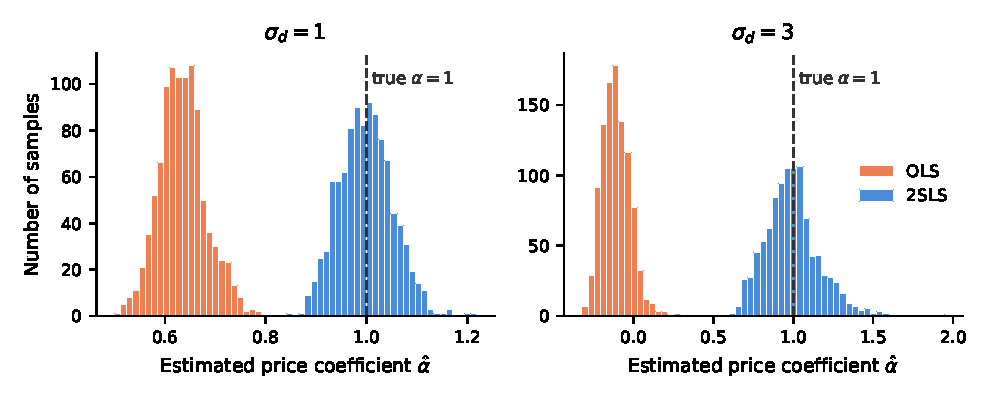
\includegraphics[width=\linewidth]{figures/ch07/mc_logit_ols_iv.pdf}
\caption{Sampling distributions of the estimated price coefficient $\hat\alpha$ in 1,000 samples of 500 duopoly
markets, for the design of \citet[Section~8]{Berry1994}. Left: $\sigma_d = 1$. Right: $\sigma_d = 3$. The dashed line
marks the true value $\alpha = 1$. OLS means are 0.635 and $-0.109$, and 2SLS means are 0.999 and 0.992. Source:
\texttt{figures/ch07/src/mc\_logit\_iv.py}.}
\label{fig:07-mc-ols-iv}
\end{figure}

\casehead{Results}
\Cref{tab:07-mc-logit} places Berry's numbers next to ours, and \cref{fig:07-mc-ols-iv} shows the sampling
distributions of $\hat\alpha$. The qualitative findings replicate. OLS underestimates the price coefficient in every
sample, while 2SLS is centered on the truth (means 1.010 and 1.002, against Berry's 0.995 and 0.979). The OLS bias is
much larger when $\xi$ explains more of mean utility. With $\sigma_d = 1$, OLS implies inelastic demand for 5.3
percent of products, and 99 of our 100 samples contain at least one such product. Berry notes that the OLS estimate
then makes firms appear to price ``on an inelastic portion of their demand curves.'' With $\sigma_d = 3$, he finds
that OLS ``sometimes'' gives $\hat\alpha < 0$. In our replication this happens in 90 of 100 samples.

Our OLS bias is larger than Berry's (mean $\hat\alpha$ of 0.638 and $-0.120$, against 0.726 and 0.181). The 2SLS
results agree closely, so the equilibrium computation and the estimators are unlikely sources of the gap. Berry does
not report every detail, such as the treatment of markets with extreme shares or how his standard errors were
computed. We report our numbers as they come out. The qualitative conclusions do not depend on the gap.

\Cref{prop:07-ols-bias} accounts for the OLS numbers. In a large simulated sample with $\sigma_d = 1$ (20,000 markets),
the projection of price on $x_j$ has slope $\Gamma = 1.847$. With $\hat\alpha_{OLS} = 0.638$ the bias in the price
coefficient is $b = 0.362$, and \eqref{eq:07-ols-bias} predicts $\plim\hat\beta_{x} = 2 - 1.847 \times 0.362 = 1.33$.
The replication mean is 1.335. The bias grows with $\sigma_d$ because the covariance between price and the error
$\sigma_d\xi_j$ scales with $\sigma_d$ twice. It scales once directly, and once through the markup, since by
\eqref{eq:07-dp-dxi} each unit of $\xi_j$ moves price by $\frac{\sigma_d s_j}{\alpha}$. The exogenous price variation
from $w_j$ and $\omega_j$ does not grow with $\sigma_d$.

The experiment also shows which instrument does the work. With $\sigma_d = 1$, the cost shifter alone gives a median
first-stage $F$ of 162. The rival's characteristic alone gives a median $F$ of 1.0, and 2SLS with it alone has a
standard deviation of 1.12 across samples. It is weak because $x$ raises cost as well as utility. In the large sample a
unit increase in $x_j$ raises marginal cost by 1.69 and price by 1.85, so the net mean utility $\beta_0 + \beta_x x_j +
\sigma_d\xi_j - \alpha p_j$ rises by only 0.15. A rival with a higher $x$ is barely more attractive.

\begin{table}[htbp]
\centering
\caption{Rival characteristics as the only instrument: duopoly versus many products.}
\label{tab:07-mc-weak}
\footnotesize
\setlength{\tabcolsep}{4.5pt}
\begin{tabular}{rrccccccc}
\toprule
$J$ & $T$ & Mean $s_0$ & s.d.\ of markups & Median $F$ & \multicolumn{2}{c}{2SLS with $z^{\mathrm{riv}}$} &
2SLS with $w$ & OLS \\
\cmidrule(lr){6-7}
 & & & & & median $\hat\alpha$ & IQR & median $\hat\alpha$ & median $\hat\alpha$ \\
\midrule
2 & 500 & 0.280 & 0.898 & 40.9 & 1.008 & [0.930, 1.082] & 1.000 & 0.483 \\
5 & 200 & 0.062 & 0.520 & 13.3 & 1.024 & [0.852, 1.201] & 1.003 & 0.534 \\
10 & 100 & 0.015 & 0.308 & 1.8 & 0.895 & [0.575, 1.346] & 0.991 & 0.557 \\
25 & 40 & 0.003 & 0.147 & 0.5 & 0.763 & [0.180, 1.369] & 0.999 & 0.578 \\
50 & 20 & 0.001 & 0.085 & 0.4 & 0.538 & [$-0.134$, 1.228] & 1.003 & 0.581 \\
\bottomrule
\end{tabular}
\par\smallskip
\parbox{\linewidth}{\footnotesize Notes: Design of \eqref{eq:07-mc-design} with $\sigma_d = 1$ and $\gamma_x = 0$, so
that $x$ does not enter marginal cost. Each sample has $N = 1{,}000$ products split into $T = \frac{1{,}000}{J}$
markets of $J$ single-product firms, with 200 samples per row. The instrument $z^{\mathrm{riv}}_{j}$ is the sum of $x$ over
the other products in the market. IQR is the interquartile range across samples. The markup standard deviation is computed within each sample and averaged. Source:
\texttt{figures/ch07/src/mc\_logit\_iv.py}.}
\end{table}

\Cref{tab:07-mc-weak} uses the same machinery to show the many-products problem of \citet{Armstrong2016}. We set
$\gamma_x = 0$, so that a rival's characteristic shifts its appeal one for one, and vary the number of products per
market $J$ with 1,000 observations in total. In duopoly the rival characteristic is a strong instrument (median $F$ of
40.9). As $J$ grows, shares shrink, markups converge to $\frac{1}{\alpha} = 1$, and their standard deviation falls from
0.90 to 0.08. The first-stage $F$ falls below 2 at $J = 10$, and the 2SLS estimate drifts toward OLS with exploding
dispersion. The cost shifter is unaffected, with medians within 0.01 of the truth in every row.

\section{The supply side: Bertrand pricing with logit demand}\label{sec:07-supply}

Combined with a model of pricing, demand estimates give markups and marginal costs and let us predict prices after
a merger or a tax. With logit demand almost everything has a closed form: markups, best responses, the equilibrium
aggregate, and pass-through. \Cref{ch:diffprod} proves these results for any ownership structure, and we restate them
here with cross-references. We then use the markups to recover marginal costs, test conduct and simulate mergers. The
closed forms make the logit a benchmark for numerical code, and they expose supply-side restrictions that mirror the
logit's restrictions on substitution. Firms set prices simultaneously, marginal costs are constant, every firm knows
all primitives (including every $\xi_j$), and the market has $M$ consumers. We drop the market index $t$. The general
theory is in \cref{ch:diffprod} and \cref{ch:blp}.

\subsection{Single-product firms}\label{sec:07-bertrand-single}

Firm $j$ sells product $j$ and earns $\pi_j = M(p_j - mc_j)s_j(\boldsymbol p)$. Write $m_j = p_j - mc_j$ for its dollar
markup.

\begin{proposition}[Logit markups with single-product firms]\label{prop:07-logit-markup}
Under logit demand, a single-product firm's best response to any vector of rival prices is characterized by its
first-order condition (\cref{prop:04-logit-br}). By \cref{prop:04-logit-markup}, in any Bertrand-Nash equilibrium
\begin{equation}\label{eq:07-logit-markup}
  p_j - mc_j = \frac{1}{\alpha(1 - s_j)}, \qquad \frac{p_j - mc_j}{p_j} = \frac{1}{\alpha p_j(1 - s_j)} =
  \frac{1}{\varepsilon_j}.
\end{equation}
Markups exceed $\frac{1}{\alpha}$ and depend on product characteristics, prices and costs only through the product's
own market share.
\end{proposition}

The markup is the single-product case of \cref{prop:04-logit-markup}. With $\frac{\partial s_j}{\partial p_j} =
-\alpha s_j(1 - s_j)$ from \cref{prop:07-logit-derivs}, the derivative of profit factors as $M s_j[1 - \alpha m_j(1 -
s_j)]$. The bracket falls strictly once $m_j > 0$ and crosses zero exactly once, and \cref{ch:diffprod} shows that the
crossing is the global maximizer. Dividing the markup by $p_j$ and using $\varepsilon_j = \alpha p_j(1 - s_j)$ gives
the Lerner form.

Two products with the same share therefore have the same dollar markup, whatever their characteristics or costs.
With small shares every markup is close to $\frac{1}{\alpha}$, so Lerner indices are roughly inversely proportional to
price. This is the supply-side image of an own elasticity that rises almost proportionally with price
(\cref{sec:07-iia}), and \cref{sec:07-limits} contrasts it with random coefficient estimates.

The first-order condition is implicit, because $s_j$ depends on $p_j$. It has a closed-form solution in terms of the
\emph{Lambert $W$ function}, defined as the inverse of $u \mapsto ue^u$ on $[0, \infty)$, so that $W(z)e^{W(z)} = z$
for $z \ge 0$ \citep{CorlessEtAl1996}. $W$ is increasing, $W(0) = 0$, and $W'(z) = \frac{W(z)}{z(1 + W(z))}$ for $z >
0$. Define
\begin{equation*}
  v_j = x_j\beta + \xi_j - \alpha\,mc_j, \qquad D_{-j} = 1 + \sum_{l \neq j} e^{\delta_l}.
\end{equation*}
The first is the mean utility product $j$ would have if priced at marginal cost, so $\delta_j = v_j - \alpha m_j$. The
second depends only on rivals' prices. Then $1 - s_j = \frac{D_{-j}}{D_{-j} + e^{\delta_j}}$, and the first-order
condition $\alpha m_j (1 - s_j) = 1$ becomes
\begin{align*}
  \alpha m_j D_{-j} &= D_{-j} + e^{v_j - \alpha m_j} \\
  (\alpha m_j - 1) D_{-j} &= e^{v_j - \alpha m_j} \\
  (\alpha m_j - 1)e^{\alpha m_j - 1} &= \frac{e^{v_j - 1}}{D_{-j}} .
\end{align*}
The last line multiplies both sides by $\frac{e^{\alpha m_j - 1}}{D_{-j}}$. It has the form $ue^u = z$ with $u = \alpha
m_j - 1$, so $u = W(z)$ and
\begin{equation}\label{eq:07-br-lambert}
  BR_j(\boldsymbol p_{-j}) = mc_j + \frac{1}{\alpha}\Bigl[1 + W\Bigl(\frac{e^{v_j - 1}}{D_{-j}}\Bigr)\Bigr].
\end{equation}
This is \eqref{eq:04-logit-br} of \cref{ch:diffprod}, where $D_{-j}$ is written $\Phi_{-j}$. The best response lies
between two bounds. As rival prices fall without limit, $D_{-j} \to \infty$ and the best
response falls to $mc_j + \frac{1}{\alpha}$. As rival prices rise without limit, $D_{-j} \to 1$ and the best response
rises to the monopoly price $mc_j + \frac{1}{\alpha}[1 + W(e^{v_j - 1})]$.

The slope of the best response follows from the chain rule. Since $\frac{\partial D_{-j}}{\partial p_l} = -\alpha
e^{\delta_l}$ for $l \neq j$, the argument $z = \frac{e^{v_j - 1}}{D_{-j}}$ satisfies $\frac{\partial z}{\partial p_l} =
\frac{\alpha z e^{\delta_l}}{D_{-j}}$, and
\begin{equation*}
  \frac{\partial BR_j}{\partial p_l} = \frac{1}{\alpha}W'(z)\frac{\partial z}{\partial p_l}
  = \frac{W(z)}{1 + W(z)}\,\frac{e^{\delta_l}}{D_{-j}} .
\end{equation*}
At the best response, $1 + W(z) = \alpha m_j = \frac{1}{1 - s_j}$, so $\frac{W(z)}{1 + W(z)} = s_j$. Also
$\frac{e^{\delta_l}}{D_{-j}} = \frac{s_l}{1 - s_j}$. Hence
\begin{equation}\label{eq:07-br-slope}
  \frac{\partial BR_j}{\partial p_l} = \frac{s_j s_l}{1 - s_j} > 0, \qquad
  \sum_{l \neq j}\frac{\partial BR_j}{\partial p_l} = s_j\,\frac{1 - s_j - s_0}{1 - s_j} < s_j .
\end{equation}
Prices are \emph{strategic complements}: a rival's price increase raises the firm's best response. The response is less
than one for one in total. The share at the best response is bounded by its monopoly value $\bar s_j =
\frac{W(e^{v_j - 1})}{1 + W(e^{v_j - 1})} < 1$, because $z \le e^{v_j - 1}$. The row sums of the Jacobian of the
best-response map are therefore below $\max_j \bar s_j < 1$ at every price vector. \Cref{prop:04-logit-br} uses this
bound to show that the map is a contraction, so the equilibrium is unique and best-response iteration converges to it
from any starting point.

\begin{figure}[htbp]
\centering
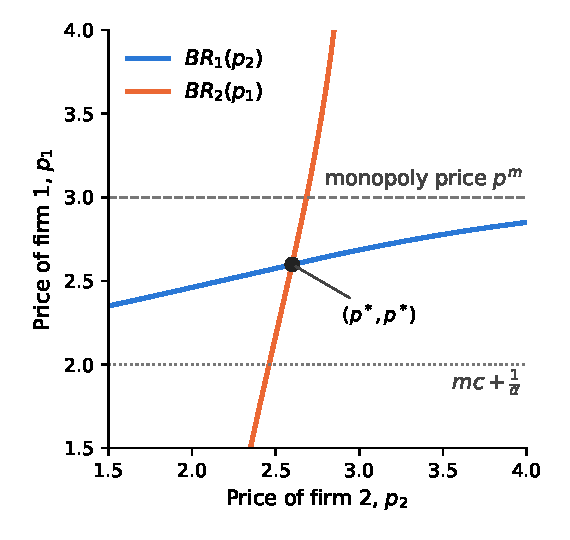
\includegraphics[width=0.52\linewidth]{figures/ch07/logit_best_response.pdf}
\caption{Best responses in a symmetric logit duopoly with an outside good, from \eqref{eq:07-br-lambert}. Both
products have $x_j\beta + \xi_j = 3$ and $mc_j = 1$, and $\alpha = 1$. The horizontal lines bound $BR_1$: it
approaches $mc + \frac{1}{\alpha} = 2$ as $p_2$ falls and the monopoly price $p^m = 3$ as $p_2$ rises. The unique
equilibrium is $p^* = 2.599$ with shares $s_j = 0.375$, where the slope of each best response is $\frac{s_j^2}{1 - s_j}
= 0.224$. Source: \texttt{figures/ch07/src/logit\_best\_response.py}.}
\label{fig:07-best-response}
\end{figure}

\Cref{fig:07-best-response} draws the two best responses of a symmetric duopoly. Each is increasing and flat, and they
cross once. At the equilibrium the markup is $p^* - mc = 1.599$, which equals $\frac{1}{\alpha(1 - s_j)} =
\frac{1}{0.625}$ up to rounding.

\subsection{Multi-product firms}\label{sec:07-bertrand-multi}

Now firm $f$ owns the set $\mathcal{J}_f$ and maximizes $\pi_f = M\sum_{k \in \mathcal{J}_f}(p_k - mc_k)s_k(\boldsymbol
p)$. The first-order condition for $j \in \mathcal{J}_f$ is
\begin{equation}\label{eq:07-multi-foc}
  s_j + \sum_{k \in \mathcal{J}_f}(p_k - mc_k)\frac{\partial s_k}{\partial p_j} = 0 .
\end{equation}
Stacking over all products with the ownership matrix $\Omega$ and the derivative matrix $\Delta$, $\Delta_{jk} =
\frac{\partial s_j}{\partial p_k}$, gives
\begin{equation}\label{eq:07-multi-foc-matrix}
  \boldsymbol s + (\Omega \odot \Delta)^\top(\boldsymbol p - \boldsymbol{mc}) = 0, \qquad
  \boldsymbol p - \boldsymbol{mc} = -\bigl[(\Omega \odot \Delta)^\top\bigr]^{-1}\boldsymbol s,
\end{equation}
as in \cref{ch:diffprod}. Because $\Omega$ is symmetric, $(\Omega \odot \Delta)^\top = \Omega \odot \Delta^\top$. With
logit demand the matrix inversion is unnecessary.

\begin{proposition}[Common markups with multi-product firms]\label{prop:07-logit-multi}
By \cref{prop:04-logit-markup}, under logit demand every solution of the first-order conditions
\eqref{eq:07-multi-foc}, and hence every Bertrand-Nash equilibrium, gives every product of firm $f$ the same dollar
markup
\begin{equation}\label{eq:07-logit-multi}
  m_f = \frac{1}{\alpha(1 - S_f)}, \qquad S_f = \sum_{k \in \mathcal{J}_f} s_k .
\end{equation}
\end{proposition}

The proof in \cref{ch:diffprod} substitutes the logit derivatives into \eqref{eq:07-multi-foc}. This gives $m_j =
\frac{1}{\alpha} + \sum_{k \in \mathcal{J}_f} s_k m_k$ for every $j \in \mathcal{J}_f$, and the right side does not
depend on $j$.

The common markup has a clean interpretation. Substitute $\frac{\partial s_j}{\partial p_j} = -\alpha s_j(1 - s_j)$
and $\frac{\partial s_k}{\partial p_j} = \alpha s_j s_k$ into \eqref{eq:07-multi-foc} and divide by $\alpha s_j(1 -
s_j)$:
\begin{equation}\label{eq:07-recapture}
  m_j = \frac{1}{\alpha(1 - s_j)} + \sum_{k \in \mathcal{J}_f,\, k \neq j} D_{jk}\, m_k, \qquad D_{jk} = \frac{s_k}{1 -
  s_j}.
\end{equation}
The first term is the single-product markup. The second is the value of the sales that a price increase on $j$
diverts to the firm's other products, where $D_{jk}$ is the logit diversion ratio (\cref{sec:07-logit-elasticities}).
A multi-product firm internalizes this recapture, so it prices above the single-product level. In the logit,
diversion is proportional to shares, so recapture depends on the firm's total share and on nothing else. The second
term of \eqref{eq:07-recapture} is the upward pricing pressure that a merger creates (\cref{ch:mergers}). Because
markups are common in dollars, the firm's cheaper products carry the higher percentage markups.

The best response of a multi-product firm also has a closed form. Holding rival prices fixed, every stationary point
of $\pi_f$ has common markups by \cref{prop:07-logit-multi}. Let $E_f = \sum_{k \in \mathcal{J}_f} e^{v_k}$ and $D_{-f} = 1 +
\sum_{l \notin \mathcal{J}_f} e^{\delta_l}$. With a common markup, $S_f = \frac{E_f e^{-\alpha m_f}}{D_{-f} + E_f
e^{-\alpha m_f}}$, and the steps that led to \eqref{eq:07-br-lambert} give
\begin{equation}\label{eq:07-br-multi}
  m_f^{BR} = \frac{1}{\alpha}\Bigl[1 + W\Bigl(\frac{E_f e^{-1}}{D_{-f}}\Bigr)\Bigr], \qquad
  p_k = mc_k + m_f^{BR} \text{ for } k \in \mathcal{J}_f .
\end{equation}
This is \eqref{eq:04-logit-br-multi} of \cref{ch:diffprod}. The firm's products enter only through the sum $E_f$, a
property that the uniqueness proof of \cref{thm:04-logit-unique} exploits.

\Cref{ex:04-logit25} solves both pricing games in one market with 25 products, five owners and $\alpha = 2$, and
\cref{tab:04-logit25} reports the results. With single-product firms, markups range from 0.502 to 0.566, all close to
$\frac{1}{\alpha} = 0.5$. Under the actual ownership each owner has one markup, equal to $\frac{1}{\alpha(1 - S_f)}$.
It ranges from 0.524 for the owner with the smallest combined share to 0.670 for the owner with the largest. Every
price rises, the outside share rises from 0.137 to 0.160, and total profit rises by about 14 percent. \Cref{app:problems}
works through the full problem.

\subsection{Existence and uniqueness of equilibrium}\label{sec:07-uniqueness}

Counterfactuals need a unique equilibrium. Without it, a merger simulation does not tell us which of several
post-merger price vectors to expect. Uniqueness can fail in general pricing games, and \cref{ch:diffprod} discusses the
conditions of \citet{CaplinNalebuff1991} for single-product firms. For the logit, uniqueness holds for any ownership
structure. The single-product case follows from Caplin and Nalebuff and from the contraction argument after
\eqref{eq:07-br-slope}. The multi-product case is due to \citet[Theorem~7, p.~279]{KonovalovSandor2010} and
\citet{NockeSchutz2018}.
In an \emph{aggregative game} each firm's profit depends on its rivals' prices only through one aggregator, and
consumer surplus is a monotone function of it \citep[p.~229, n.~127]{AskerNocke2021}. The logit pricing game is
aggregative, and its aggregator is the inclusive sum $\Lambda = 1 + \sum_k e^{\delta_k}$, which \cref{ch:diffprod}
writes as $\Phi$.

\begin{proposition}[Existence and uniqueness]\label{prop:07-logit-unique}
With logit demand, constant marginal costs and any partition of the products among firms, the Bertrand-Nash pricing
game has exactly one equilibrium. This is \cref{thm:04-logit-unique}.
\end{proposition}

The proof of \cref{thm:04-logit-unique} reduces the equilibrium to one equation in one unknown, the aggregate
$\Lambda$. Each firm sets the common markup of \cref{prop:07-logit-multi}, so its combined share is $S_f = \frac{E_f
e^{-\alpha m_f}}{\Lambda}$, with $E_f$ as in \eqref{eq:07-br-multi}. Substituting $\alpha m_f = \frac{1}{1 - S_f}$
gives
\begin{equation}\label{eq:07-share-aggregate}
  S_f\, e^{\frac{1}{1 - S_f}} = \frac{E_f}{\Lambda} .
\end{equation}
The left side rises strictly from 0 to $+\infty$ as $S_f$ rises from 0 to 1. Each firm's share is therefore a
continuous and strictly decreasing function $S_f(\Lambda)$ of the aggregate. The inside shares and the outside share
$\frac{1}{\Lambda}$ add up to one, so the equilibrium aggregate solves
\begin{equation}\label{eq:07-psi}
  \Psi(\Lambda) \equiv \sum_f S_f(\Lambda) + \frac{1}{\Lambda} = 1 .
\end{equation}
The function $\Psi$ is strictly decreasing, exceeds one at $\Lambda = 1$ and tends to zero as $\Lambda \to \infty$.
It has exactly one root $\Lambda^* > 1$, and the root pins down every share, markup and price.

The characterization doubles as an algorithm: solve \eqref{eq:07-psi} by bisection and read off shares, markups and
prices. Best-response iteration with \eqref{eq:07-br-multi}, the markup fixed point $\boldsymbol p \leftarrow
\boldsymbol{mc} + \frac{1}{\alpha(1 - S_f(\boldsymbol p))}$, and Newton's method are common alternatives. In the
market of \cref{ex:04-logit25}, $\Lambda^* = 7.314$ with single-product firms and $6.246$ with multi-product firms,
equal to $\frac{1}{s_0}$ in each case (\cref{ex:04-logit25-unique}). With non-logit demand uniqueness is not
guaranteed, and restarting the solver from many points is the practical check (\cref{ch:blp}).

\subsection{Pass-through}\label{sec:07-passthrough}

The \emph{pass-through rate} $\rho = \frac{\dd p}{\dd mc}$ measures how much of a cost change reaches the price
(\cref{ch:theory}). It governs the incidence of taxes, the effect of exchange rates on import prices, and the price
effect of merger efficiencies.

\begin{proposition}[Logit pass-through]\label{prop:07-logit-passthrough}
Hold rivals' prices fixed. By parts (i) and (iii) of \cref{prop:04-passthrough}, the following hold.
\begin{enumerate}[label=(\roman*)]
  \item A single-product firm passes through $\rho_j = \frac{\dd p_j}{\dd mc_j} = 1 - s_j$ of an increase in its
    marginal cost.
  \item A multi-product firm facing the same increase in the marginal cost of all its products raises all its prices by
    $\rho_f = 1 - S_f$ per unit of cost.
\end{enumerate}
In both cases pass-through is below one and falls with the firm's share.
\end{proposition}

The proof in \cref{ch:diffprod} differentiates the markup condition $\alpha m_f(1 - S_f) = 1$. A common cost increase
$\dd mc$ lowers the firm's combined share, and the common markup falls by $S_f\,\dd mc$, so each price rises by $(1 -
S_f)\,\dd mc$. A single-product firm is the case $S_f = s_j$.

Pass-through below one is the logit instance of a general result for log-concave demand. For a single-product firm
with demand $q(p)$ at fixed rival prices, \eqref{eq:02-pt-logcurv} gives
\begin{equation*}
  \rho = \frac{\dd p}{\dd mc} = \frac{1}{2 - \frac{q q''}{(q')^2}} ,
\end{equation*}
and $\rho < 1$ exactly when demand is log-concave at the optimum (\cref{cor:02-bulow-pfleiderer}).
\citet{BulowPfleiderer1983} write the same pass-through rate in terms of the demand elasticity and its slope, as
restated by \citet[p.~18 of the 2008 working paper]{FarrellShapiro2010}. \citet{WeylFabinger2013} develop pass-through
as a general tool for incidence under imperfect competition. Holding rivals' prices fixed, logit demand is log-concave
in own price:
\begin{equation*}
  \frac{\dd \ln s_j}{\dd p_j} = -\alpha(1 - s_j), \qquad \frac{\dd^2 \ln s_j}{\dd p_j^2} = \alpha\frac{\dd s_j}{\dd p_j}
  = -\alpha^2 s_j(1 - s_j) < 0 .
\end{equation*}
With $q = s_j$, $q' = -\alpha s_j(1 - s_j)$ and $q'' = \alpha^2 s_j(1 - s_j)(1 - 2s_j)$, the ratio $\frac{q
q''}{(q')^2}$ equals $\frac{1 - 2s_j}{1 - s_j}$, and the general formula returns $\rho_j = 1 - s_j$.
In the market of \cref{ex:04-logit25} the largest owner has $S_f = 0.2536$, and a numerical derivative of
\eqref{eq:07-br-multi} gives pass-through 0.7464, equal to $1 - S_f$. The proposition holds rivals' prices fixed.
When a cost shock hits all firms, rivals raise their prices as well. By strategic complementarity
\eqref{eq:07-br-slope}, equilibrium pass-through then exceeds $1 - s_j$ (\cref{cor:04-passthrough-eq}).

\begin{figure}[htbp]
\centering
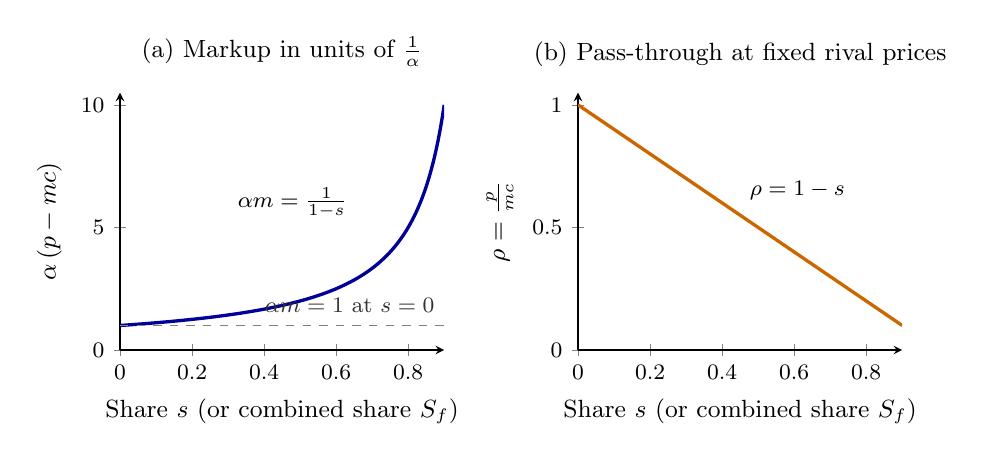
\begin{tikzpicture}
\begin{axis}[
  name=leftax, width=0.47\linewidth, height=0.40\linewidth,
  xmin=0, xmax=0.9, ymin=0, ymax=10.5,
  xlabel={Share $s$ (or combined share $S_f$)}, ylabel={$\alpha\,(p - mc)$},
  title={(a) Markup in units of $\frac{1}{\alpha}$},
  title style={font=\small}, label style={font=\small}, tick label style={font=\footnotesize},
  domain=0:0.9, samples=200, axis lines=left]
  \addplot[very thick, blue!60!black] {1/(1-x)};
  \node[font=\footnotesize, anchor=west] at (axis cs:0.30,6.0) {$\alpha m = \frac{1}{1 - s}$};
  \addplot[dashed, gray] coordinates {(0,1) (0.9,1)};
  \node[font=\footnotesize, anchor=south east, gray!40!black] at (axis cs:0.90,1.15) {$\alpha m = 1$ at $s = 0$};
\end{axis}
\begin{axis}[
  at={(leftax.east)}, anchor=west, xshift=1.7cm,
  width=0.47\linewidth, height=0.40\linewidth,
  xmin=0, xmax=0.9, ymin=0, ymax=1.05,
  xlabel={Share $s$ (or combined share $S_f$)}, ylabel={$\rho = \frac{\dd p}{\dd mc}$},
  title={(b) Pass-through at fixed rival prices},
  title style={font=\small}, label style={font=\small}, tick label style={font=\footnotesize},
  domain=0:0.9, samples=50, axis lines=left]
  \addplot[very thick, orange!80!black] {1-x};
  \node[font=\footnotesize, anchor=west] at (axis cs:0.45,0.65) {$\rho = 1 - s$};
\end{axis}
\end{tikzpicture}
\caption{Logit markups and pass-through as functions of the firm's share. Panel (a): the dollar markup times $\alpha$,
from \cref{prop:07-logit-markup,prop:07-logit-multi}. Panel (b): the pass-through rate of
\cref{prop:07-logit-passthrough}. For a multi-product firm, read the horizontal axis as $S_f$.}
\label{fig:07-markups}
\end{figure}

\Cref{fig:07-markups} summarizes the two results. Markups rise and pass-through falls with the firm's share, and
nothing else about the product matters. The link to merger analysis is direct. \citet{FarrellShapiro2010} define the
upward pricing pressure on product $j$ after a merger with the owner of $k$ as $D_{jk}m_k$, the second term of
\eqref{eq:07-recapture}. They evaluate it at pre-merger prices and before any credit for cost savings (p.~9 of their
2008 working paper). \citet[p.~231]{AskerNocke2021} state the same definition and read it as the merged firm's
opportunity cost of keeping the price of $j$ at its pre-merger level. It acts like a cost increase on $j$, so to first
order the price of $j$ rises by
$\rho_j D_{jk}m_k = (1 - s_j)\frac{s_k}{1 - s_j}m_k = s_k m_k$ under logit demand. \Cref{ch:mergers} develops this
approximation and its limits.

\subsection{Recovering marginal costs and joint estimation}\label{sec:07-cost-recovery}

Given an estimate $\hat\alpha$ and an assumed ownership structure, the first-order conditions deliver marginal costs
without any cost data. Suppose marginal cost is linear in observed cost shifters $w_{jt}$ and a cost shock
$\omega_{jt}$, $mc_{jt} = w_{jt}\gamma + \omega_{jt}$. By \cref{prop:07-logit-multi},
\begin{equation}\label{eq:07-logit-supply}
  p_{jt} = w_{jt}\gamma + \frac{1}{\alpha(1 - S_{ft})} + \omega_{jt},
  \qquad \widehat{mc}_{jt} = p_{jt} - \frac{1}{\hat\alpha(1 - S_{ft})} .
\end{equation}
With single-product firms ($S_{ft} = s_{jt}$) the first equation is equation (31) of \citet[p.~255]{Berry1994},
whose parameters are $\gamma$ and $\frac{1}{\alpha}$. His general version (equation 29) lets cost depend on output and
writes the markup as $\frac{s_j}{\alpha}\bigl(\frac{\partial s_j}{\partial\delta_j}\bigr)^{-1}$, which covers any demand
model. The
nested logit version is \cref{prop:07-nl-markup}.

There are two ways to estimate $\gamma$. The \emph{two-step} approach regresses $\widehat{mc}_{jt}$ on $w_{jt}$ by
OLS. It is consistent when $\E[w_{jt}^\top\omega_{jt}] = 0$ and $\hat\alpha$ is consistent. Its usual standard errors
are wrong, because the dependent variable is a \emph{generated regressand}. The error in the implied cost is
\begin{equation*}
  \widehat{mc}_{jt} - mc_{jt} = \frac{1}{\alpha(1 - S_{ft})} - \frac{1}{\hat\alpha(1 - S_{ft})} \approx
  \frac{\hat\alpha - \alpha}{\alpha^2(1 - S_{ft})} ,
\end{equation*}
which is nearly common to all products when shares are small, so it loads on the intercept of the cost regression.
The simulated market of \cref{sec:08-worked-logit}, which \cref{app:problems} works through, shows the size of the
effect. A market bootstrap that re-estimates $\alpha$ raises the intercept's standard error there from 0.016 to 0.072,
while the slopes' standard errors barely move. Valid inference uses
such a bootstrap or the sandwich of a stacked GMM problem \citep{Newey1984}. Negative implied costs signal a problem
with the demand estimates or the conduct assumption.

The \emph{joint} approach estimates demand and supply together. Let $\theta = (\beta, \alpha, \gamma)$ and define the
two structural errors
\begin{equation}\label{eq:07-joint-errors}
  \xi_{jt}(\theta) = y_{jt} - x_{jt}\beta + \alpha p_{jt}, \qquad
  \omega_{jt}(\theta) = p_{jt} - \frac{1}{\alpha(1 - S_{ft})} - w_{jt}\gamma .
\end{equation}
With demand instruments $z^d_{jt}$ and supply instruments $z^s_{jt}$, the moment conditions are $\E[z^{d\top}_{jt}
\xi_{jt}(\theta)] = 0$ and $\E[z^{s\top}_{jt}\omega_{jt}(\theta)] = 0$. GMM minimizes $\bar g(\theta)^\top W \bar
g(\theta)$ for the stacked sample moments
\begin{equation}\label{eq:07-joint-gmm}
  \bar g(\theta) = \frac{1}{N}\sum_t\sum_{j \in \mathcal{J}_t}
  \begin{pmatrix} z^{d\top}_{jt}\,\xi_{jt}(\theta) \\ z^{s\top}_{jt}\,\omega_{jt}(\theta) \end{pmatrix} .
\end{equation}
For a given $\alpha$ both errors are linear in $(\beta, \gamma)$, which can be concentrated out, so the search is over
$\alpha$ alone. The markup term is endogenous, because $S_{ft}$ depends on prices and hence on $\omega_{jt}$.
\citet[p.~255]{Berry1994} lists its instruments: excluded demand characteristics, characteristics of other firms, and
market population when markets differ in size.

Joint estimation helps when demand instruments are weak, because the markup term carries information about $\alpha$
if the supply instruments overidentify $\gamma$. It also exploits any correlation between $\xi$ and $\omega$, it is
where conduct enters when conduct is tested, and it gives correct standard errors for $\gamma$. The cost is
robustness. A wrong ownership or conduct assumption contaminates the demand estimates through the shared $\alpha$.
Berry notes that joint estimation ``would take into account the cross-equation restrictions on parameters.''
\Cref{ch:blp} develops joint estimation with random coefficients, where the gains are larger.

\subsection{Testing conduct and ownership with logit demand}\label{sec:07-conduct}

The same first-order conditions can be evaluated under different assumptions about who sets which price. Let a
\emph{pricing coalition} be a set of products whose prices are chosen jointly. By \cref{prop:07-logit-multi}, a
coalition $A$ sets the common markup $\frac{1}{\alpha(1 - S_A)}$, where $S_A$ is its combined share. Implied Lerner
indices under four structures are therefore analytic:
\begin{equation}\label{eq:07-conduct-margins}
  \underbrace{\frac{1}{\alpha p_j(1 - s_j)}}_{\text{single product}}, \qquad
  \underbrace{\frac{1}{\alpha p_j(1 - S_f)}}_{\text{actual ownership}}, \qquad
  \underbrace{\frac{1}{\alpha p_j(1 - S_G)}}_{\text{joint pricing of } G}, \qquad
  \underbrace{\frac{1}{\alpha p_j s_0}}_{\text{monopoly}},
\end{equation}
where $G$ is a group of colluding products, and monopoly uses $1 - \sum_{k \ge 1}s_k = s_0$. Comparing the predicted
margins with observed margins, or with outside information on costs, tests the structures. Only $\hat\alpha$ and the
shares are needed.

\citet[Section~5.3]{Nevo2001} carries out this comparison for cereal, and \cref{tab:07-nevo-margins} reproduces the
logit column of his Table VIII. It uses the price coefficient of column (ix) of \cref{tab:07-nevo-logit}. Because only
shares are needed, the logit margins can include brands outside the 25 in the sample, which the full model cannot
\citep[pp.~332--333]{Nevo2001}.

\begin{table}[htbp]
\centering
\caption{Median price-cost margins in ready-to-eat cereal under alternative pricing structures, logit demand.}
\label{tab:07-nevo-margins}
\footnotesize
\begin{tabular}{lc}
\toprule
 & Logit \\
 & (Table V, column ix) \\
\midrule
Single-product firms & 33.6\% \\
 & (31.8\%--35.6\%) \\
Current ownership of 25 brands & 35.8\% \\
 & (33.9\%--38.0\%) \\
Joint ownership of 25 brands & 41.9\% \\
 & (39.7\%--44.4\%) \\
Current ownership of all brands & 37.2\% \\
 & (35.2\%--39.4\%) \\
Monopoly or perfect price collusion & 54.0\% \\
 & (51.1\%--57.3\%) \\
\bottomrule
\end{tabular}
\par\smallskip
\parbox{\linewidth}{\footnotesize Notes: Source: \citet[Table~VIII, p.~333]{Nevo2001}, logit column. Margins are
$\frac{p - mc}{p}$. Entries are medians over 27,862 brand-city-quarter observations, with 95 percent confidence
intervals for the median in parentheses, based on the asymptotic distribution of the demand estimates. The logit
computation is analytical. \Cref{tab:08-nevo-margins} reproduces the full table, including the random coefficients
column.}
\end{table}

Nevo compares the predictions with crude accounting estimates. The gross retail margin is about 46.0 percent, and the
gap between national brands and private labels gives a lower bound of about 31 percent \citep[pp.~333--334]{Nevo2001}.
His full random coefficients model predicts a median margin of 35.8 percent with single-product firms. It is 42.2
percent (interval 29.1 to 55.8) under current ownership and 72.6 percent (62.2 to 97.2) under joint ownership of the
25 brands (\cref{tab:08-nevo-margins}). Using these intervals, he rejects joint profit maximization by the 25 brands and
cannot reject multi-product Nash pricing. The logit column tells a different story. Joint ownership of the 25 brands
raises the logit margin only from 35.8 to 41.9 percent, against 42.2 to 72.6 percent in the full model. With logit
margins, joint ownership comes closer to the accounting margin than current ownership does, so a logit-based test
could point toward collusion.

The logit understates the effect of joint pricing because of IIA. A coalition's markup depends only on
$\frac{1}{1 - S_G}$. With a market of one serving per person per day the outside share is large, so $S_G$ is far from
one even for 25 brands. Diversion is proportional to shares (\cref{sec:07-iia}), so most of the sales a brand loses go
to the outside good, and merging brands recaptures little. In the random coefficient model cereals are closer
substitutes for each other than for the outside good, so joint pricing recaptures much more. The assumed demand model
shapes the conduct test as much as the data do.

\citet[p.~874]{BerryLevinsohnPakes1995} make the same point for cars. Their IV logit implies that ``all models have
about the same mark-up,'' from \$4,630 for the BMW to \$4,805 for the Chevy Cavalier. Shares measured against all
households are tiny, so markups are close to $\frac{1}{\hat\alpha} = \frac{1}{0.216}$ thousand dollars, about \$4,630.
Differences come only from the number of models a parent firm sells. GM sells the most and has the highest markups,
while BMW has, ``quite counter-intuitively,'' the lowest. If BMW's combined share is negligible,
\eqref{eq:07-logit-multi} and $1 - \frac{4{,}630}{4{,}805} \approx 0.036$ imply that GM's models together sold to
roughly 3.6 percent of households. \Cref{sec:07-limits-markups} translates these dollar markups into Lerner
indices, and the random coefficient markups of \cref{ch:blp} vary far more across models.

Comparing implied margins across ownership structures is an alternative to estimating a conduct parameter
(\cref{ch:conduct}). It sidesteps the problem raised by \citet[p.~227]{Corts1999}, who shows that in a dynamic
oligopoly model the estimated conduct parameter can mismeasure market power severely. \citet{Bresnahan1987} applies
a nested test of this kind with the vertical model (\cref{ch:discrete}).

Logit merger simulation follows directly. \citet[p.~230]{AskerNocke2021} credit \citet{HausmanLeonardZona1994},
\citet{WerdenFroeb1994} and \citet{Nevo2000b} with pioneering \emph{merger simulation}, which has three steps. The
first estimates pre-merger demand. The second recovers pre-merger marginal costs from an assumption on pre-merger
conduct, typically static Bertrand-Nash pricing. The third computes the post-merger equilibrium under assumptions on
post-merger conduct and on merger-related cost savings, holding demand and the product set fixed. Werden and Froeb
carry out these steps with logit demand. The first two steps are then analytic, and the third reduces to one
equation in one unknown.
Estimate $\alpha$, recover marginal
costs from \eqref{eq:07-logit-supply} under the pre-merger ownership, and solve \eqref{eq:07-psi} under the
post-merger ownership. If firms $f$ and $f'$ merge, the merged firm sets one
markup $\frac{1}{\alpha(1 - S_f - S_{f'})}$ at post-merger shares, and rivals respond. Because diversion follows
shares, the predicted dollar price effects depend only on $\hat\alpha$, the ownership structure and the pre-merger
shares (\cref{ch:mergers}). When the size of the cost savings is unknown, the third step can instead find the
smallest savings that leave consumer surplus unchanged \citep[pp.~230--231]{AskerNocke2021}.

\section{GEV models and the nested logit}\label{sec:07-nested}

The logit restricts substitution because its taste shocks are independent across products (\cref{sec:07-iia}).
A consumer who leaves product $j$ after a price increase is no more likely than anyone else to choose a
product similar to $j$. Two routes break this property while keeping the model estimable from market shares.
The first correlates the shocks of products that the analyst groups together. It leads to the generalized
extreme value family and to the nested logit. The second lets taste coefficients vary across consumers. It
leads to the random coefficients logit of \cref{ch:blp}. This section develops the first route.
\Cref{sec:07-welfare} then uses both the logit and the nested logit to measure consumer welfare.

\subsection{Generalized extreme value models}\label{sec:07-gev}

We work with an additive random utility model. Consumer $i$ obtains $u_{ij} = V_{ij} + \epsilon_{ij}$ from
alternative $j = 0, 1, \dots, J$, where $V_{ij}$ is the deterministic part of utility. Throughout this
subsection we drop the consumer index and write $V = (V_0, \dots, V_J)$ and $y_j = e^{V_j}$. The choice
probability of $j$ is $P_j(V)$. The \emph{social surplus function} is the expected maximum utility,
\begin{equation}\label{eq:07-surplus}
\mathcal{W}(V) = \E\Big[\max_{j = 0, \dots, J}\,(V_j + \epsilon_j)\Big].
\end{equation}
The logit assumes that the $\epsilon_j$ are independent type-I extreme value (Gumbel) variables.
\citet{McFadden1978} found a class of correlated distributions that keeps the closed forms of the logit. The class
is indexed by a function of $J + 1$ positive arguments.

\begin{definition}[GEV generating function]\label{def:07-gev}
A function $H : \R^{J+1}_+ \to \R_+$ is a \emph{GEV generating function} if it has the following three
properties.
\begin{enumerate}[label=(G\arabic*)]
  \item $H$ is homogeneous of degree one: $H(\lambda y) = \lambda H(y)$ for every $\lambda > 0$.
  \item $H(y) \to \infty$ as $y_j \to \infty$, for each $j$.
  \item For any $r \ge 1$ distinct indices $j_1, \dots, j_r$, the mixed partial derivative
  $\frac{\partial^r H}{\partial y_{j_1}\cdots\partial y_{j_r}}$ exists, is continuous, and is nonnegative when
  $r$ is odd and nonpositive when $r$ is even.
\end{enumerate}
\end{definition}

We write $H_j$ and $H_{jk}$ for the first and second partial derivatives of $H$. Condition (G1) produces the
closed forms below. Condition (G2) makes each marginal distribution proper. Condition (G3) makes the function in
part (i) of the next proposition a joint distribution function with a nonnegative density. The notation follows
\citet[p.~1421]{McFadden1984}, who calls the function $H$. \Cref{thm:06-gev} states and proves the first
three parts of the next result. We restate them here together with two parts that this chapter also uses, the
gradient property (iv) and the derivative formula (v).

\begin{proposition}[McFadden's GEV theorem]\label{prop:07-gev}
Let $H$ be a GEV generating function and let $y = (e^{V_0}, \dots, e^{V_J})$.
\begin{enumerate}[label=(\roman*)]
  \item $F(\epsilon_0, \dots, \epsilon_J) = \exp\big[-H(e^{-\epsilon_0}, \dots, e^{-\epsilon_J})\big]$ is the
  distribution function of a random vector whose marginals are Gumbel.
  \item If $\epsilon$ has distribution $F$, the choice probabilities are
  \begin{equation}\label{eq:07-gev-prob}
  P_j(V) = \frac{y_j H_j(y)}{H(y)} = \frac{\partial \ln H(e^{V_0}, \dots, e^{V_J})}{\partial V_j}.
  \end{equation}
  \item The maximum utility $\max_j(V_j + \epsilon_j)$ is Gumbel with location $\ln H(y)$ and scale one, so that
  \begin{equation}\label{eq:07-gev-surplus}
  \mathcal{W}(V) = \ln H(y) + \gamma_E ,
  \end{equation}
  where $\gamma_E \approx 0.5772$ is Euler's constant.
  \item (Williams, Daly and Zachary.) The social surplus function is differentiable and
  $\frac{\partial \mathcal{W}(V)}{\partial V_j} = P_j(V)$ for every $j$.
  \item For all $j$ and $k$,
  \begin{equation}\label{eq:07-gev-deriv}
  \frac{\partial P_j}{\partial V_k} = P_j\big(\indic\{j = k\} - P_k\big) + \frac{y_j y_k H_{jk}(y)}{H(y)} .
  \end{equation}
\end{enumerate}
\end{proposition}

\begin{proof}
Parts (i), (ii) and (iii) are parts (a), (b) and (c) of \cref{thm:06-gev}. Part (i) is the theorem of
\citet{McFadden1978}, and the proof of \cref{thm:06-gev} derives (ii) and (iii) from it by homogeneity. Part (iv) is
part (ii) of \cref{thm:06-wdz}, which holds for every additive random utility model. In the GEV case it also follows
by differentiating \eqref{eq:07-gev-surplus} and applying (ii). Only (v) is new.

For (v), take logs in (ii): $\ln P_j = V_j + \ln H_j(y) - \ln H(y)$. Differentiate with respect to $V_k$, using
$\frac{\partial y_k}{\partial V_k} = y_k$:
\begin{equation*}
\frac{\partial \ln P_j}{\partial V_k} = \indic\{j = k\} + \frac{y_k H_{jk}(y)}{H_j(y)} - \frac{y_k H_k(y)}{H(y)}
= \indic\{j = k\} + \frac{y_k H_{jk}(y)}{H_j(y)} - P_k .
\end{equation*}
Multiplying by $P_j = \frac{y_jH_j}{H}$ gives \eqref{eq:07-gev-deriv}.
\end{proof}

Part (v) shows what correlation buys. For $j \neq k$ the logit term $-P_jP_k$ is the cross derivative of a model
with independent shocks and the same probabilities. The second term $\frac{y_jy_kH_{jk}}{H}$ is nonpositive by
(G3). A GEV model therefore implies at least as much substitution between $j$ and $k$ as the logit at the same
choice probabilities, and $H_{jk}$ measures the excess. The formula is symmetric in $j$ and $k$, which is the
counterpart of Slutsky symmetry (\cref{cor:06-wdz}). With mean utilities $V_k = \delta_k$ and
$\delta_k = x_k\beta - \alpha p_k + \xi_k$, price derivatives follow from
$\frac{\partial s_j}{\partial p_k} = -\alpha\frac{\partial P_j}{\partial \delta_k}$.

\casehead{Two generating functions}
The logit is the case $H(y) = \sum_{j=0}^J y_j$. Its first derivatives equal one and all higher derivatives vanish,
so (ii) gives $P_j = \frac{y_j}{\sum_k y_k}$ and (v) gives the logit derivatives of \cref{prop:07-logit-derivs}.
The \emph{nested logit} groups the inside products into nests. Partition the inside products into
$G$ mutually exclusive and exhaustive nests $g = 1, \dots, G$, and place the outside good alone in nest $0$. For
a nesting parameter $\sigma$, let
\begin{equation}\label{eq:07-nl-H}
H(y) = y_0 + \sum_{g=1}^G D_g(y)^{1 - \sigma}, \qquad D_g(y) = \sum_{j \in g} y_j^{\frac{1}{1-\sigma}} .
\end{equation}

\begin{lemma}[Consistency of the nested logit]\label{lem:07-nl-gev}
The function \eqref{eq:07-nl-H} is a GEV generating function for every $\sigma \in [0, 1)$. If $\sigma < 0$ and
some nest contains two or more products, it violates (G3).
\end{lemma}

\begin{proof}
For (G1), $D_g(\lambda y) = \lambda^{\frac{1}{1-\sigma}}D_g(y)$, so $D_g(\lambda y)^{1-\sigma} = \lambda D_g(y)^{1-\sigma}$.
For (G2), if $y_j \to \infty$ with $j \in g$, then $D_g \to \infty$ and $D_g^{1-\sigma} \to \infty$ because
$1 - \sigma > 0$. The outside good enters linearly.

For (G3), a mixed partial derivative over indices from two different nests is zero, which satisfies the weak sign
condition. Take distinct indices $j_1, \dots, j_r$ in the same nest $g$. Write $\varphi(D) = D^{1-\sigma}$ and
$a_j = \frac{\partial D_g}{\partial y_j} = \frac{1}{1-\sigma}y_j^{\frac{\sigma}{1-\sigma}} \ge 0$. Each $a_j$ depends on
$y_j$ alone, so the chain rule gives
\begin{equation*}
\frac{\partial^r H}{\partial y_{j_1}\cdots\partial y_{j_r}} = \varphi^{(r)}(D_g)\prod_{m=1}^r a_{j_m} .
\end{equation*}
The successive derivatives of $\varphi$ are $\varphi'(D) = (1-\sigma)D^{-\sigma}$,
$\varphi''(D) = -\sigma(1-\sigma)D^{-\sigma-1}$, $\varphi'''(D) = \sigma(\sigma+1)(1-\sigma)D^{-\sigma-2}$, and in general
\begin{equation*}
\varphi^{(r)}(D) = (-1)^{r-1}(1-\sigma)\prod_{m=0}^{r-2}(\sigma + m)\,D^{1-\sigma-r}, \qquad r \ge 2 .
\end{equation*}
For $\sigma \in [0, 1)$ every factor in the product is nonnegative, so the sign is $(-1)^{r-1}$, as (G3) requires.
If $\sigma < 0$, then $\varphi''(D) > 0$ and the second mixed derivative of two products in the same nest is
positive.
\end{proof}

The parameter range has an empirical counterpart. \citet[pp.~1425--1426]{McFadden1984} notes that estimates of
the nesting parameters outside the unit interval violate the ranking of cross elasticities implied by the tree,
and may indicate a misspecified tree. In the notation of \citet{BorschSupan1990}, our $1 - \sigma$ is the
dissimilarity parameter. He shows that values with $\sigma < 0$ can still be consistent with utility maximization
on a restricted region of mean utilities (Section~4 and Theorem~1, pp.~377--381). By Theorem~1, it suffices that
the mixed partial derivatives of the choice probabilities be nonnegative on that region. In the two-level model
this requires the choice probabilities of the nests to be large enough (Theorem~2, p.~385). With two nests of two
alternatives each and a common $\sigma < -1$, these requirements conflict and no such region exists (p.~385).
Applied work treats $\sigma \in [0, 1)$ as the admissible range. The next two subsections derive the nested logit a second way,
from an explicit utility model.

\subsection{The nested logit model}\label{sec:07-nl-model}

The nested logit relaxes IIA by grouping products. Within a nest, consumers substitute as in the logit. Products in
different nests have less in common, so they are weaker substitutes. The idea parallels the grouping of goods in
multi-stage budgeting (\cref{ch:aids}), and the same analyst judgment determines the groups.

\begin{assumption}[Nested logit]\label{asm:07-nl}
The inside products of market $t$ are partitioned into nests $g = 1, \dots, G$, and the outside good forms nest
$0$ by itself. The utility of consumer $i$ from product $j$ in nest $g$ is
\begin{equation}\label{eq:07-nl-utility}
u_{ij} = \delta_j + \zeta_{ig} + (1 - \sigma)\epsilon_{ij}, \qquad \delta_j = x_j\beta - \alpha p_j + \xi_j ,
\end{equation}
and the utility of the outside good is a standard Gumbel variable $\epsilon_{i0}$. The shocks $\epsilon_{ij}$ are
i.i.d.\ standard Gumbel. The nest tastes $\zeta_{ig}$ are i.i.d.\ across consumers and nests with the distribution
$C(\sigma)$ of \cref{lem:07-cardell}, and they are independent of the $\epsilon_{ij}$. The nesting parameter
satisfies $0 \le \sigma < 1$.
\end{assumption}

The term $\zeta_{ig}$ is common to all products in nest $g$ for consumer $i$. A consumer with a high draw likes
every product of the nest, so the utilities of products in the same nest are positively correlated.
\citet[p.~252]{Berry1994} points out that \eqref{eq:07-nl-utility} is a random coefficients model. Let $d_{jh}$
equal one if $j \in h$. Then $\zeta_{ig} = \sum_h d_{jh}\zeta_{ih}$ for $j \in g$, so the nest taste is a random
coefficient on the nest dummies, with a distribution tied to $\sigma$. Unlike the full random coefficients model, correlation can depend only on
groupings fixed before estimation, never on continuous characteristics. \Citet[p.~524]{Nevo2000a} makes the same
point, and \citet{Cardell1997} shows that the two descriptions of the nested logit are equivalent. The
distribution of $\zeta_{ig}$ is chosen so that the composite shock remains Gumbel.

\begin{lemma}[\citealp{Cardell1997}]\label{lem:07-cardell}
For every $\sigma \in [0, 1)$ there is a unique distribution $C(\sigma)$ with the following property. If
$\zeta \sim C(\sigma)$ and $\epsilon$ is a standard Gumbel variable independent of $\zeta$, then
$\zeta + (1 - \sigma)\epsilon$ is a standard Gumbel variable. Equivalently, the random variable
$X = e^{\frac{\zeta}{1-\sigma}}$ satisfies
\begin{equation}\label{eq:07-cardell-laplace}
\E\big[e^{-cX}\big] = \exp\big(-c^{1-\sigma}\big) \qquad \text{for every } c > 0 .
\end{equation}
\end{lemma}

We do not prove existence, which \citet{Cardell1997} establishes along with the density of $\zeta$. The
equivalence is a short computation. Conditioning on $\zeta$,
\begin{equation*}
\Pr\big(\zeta + (1-\sigma)\epsilon \le t\big) = \E\Big[\exp\Big(-e^{-\frac{t - \zeta}{1-\sigma}}\Big)\Big]
= \E\big[e^{-cX}\big], \qquad c = e^{-\frac{t}{1-\sigma}} .
\end{equation*}
The standard Gumbel distribution function is $\exp(-e^{-t}) = \exp(-c^{1-\sigma})$, which gives
\eqref{eq:07-cardell-laplace}. A Laplace transform determines a distribution, which explains uniqueness. The
function $c \mapsto \exp(-c^{a})$ with $0 < a \le 1$ is the Laplace transform of the positive stable law of index
$a$ \citep{Feller1971}. So $\zeta$ is $(1-\sigma)$ times the logarithm of a positive stable variable of index
$1 - \sigma$. At $\sigma = 0$ the stable variable equals one and $\zeta = 0$.

\begin{proposition}[Nested logit shares]\label{prop:07-nl-shares}
Under \cref{asm:07-nl}, define the inclusive sum of nest $g$ as
$D_g = \sum_{k \in g} e^{\frac{\delta_k}{1-\sigma}}$. Then the within-nest share, the nest share, the product share
and the outside share are
\begin{equation}\label{eq:07-nl-share}
s_{j \mid g} = \frac{e^{\frac{\delta_j}{1-\sigma}}}{D_g}, \qquad
s_g = \frac{D_g^{1-\sigma}}{1 + \sum_{h=1}^G D_h^{1-\sigma}}, \qquad
s_j = s_{j \mid g}\,s_g, \qquad
s_0 = \frac{1}{1 + \sum_{h=1}^G D_h^{1-\sigma}} .
\end{equation}
The composite shocks $\zeta_{ig} + (1-\sigma)\epsilon_{ij}$ have the GEV distribution generated by
\eqref{eq:07-nl-H}.
\end{proposition}

\begin{proof}
We give two derivations. The first uses \cref{prop:07-gev}. The second builds the shares nest by nest.

\emph{GEV derivation.} Fix a nest $g$ and numbers $t_j$ for $j \in g$. Conditioning on $\zeta_{ig}$ and using the
independence of the $\epsilon_{ij}$,
\begin{equation*}
\Pr\big(\zeta_{ig} + (1-\sigma)\epsilon_{ij} \le t_j \text{ for all } j \in g\big)
= \E\Big[\prod_{j\in g}\exp\Big(-e^{-\frac{t_j - \zeta_{ig}}{1-\sigma}}\Big)\Big]
= \E\Big[\exp\Big(-X\sum_{j \in g}e^{-\frac{t_j}{1-\sigma}}\Big)\Big],
\end{equation*}
with $X = e^{\frac{\zeta_{ig}}{1-\sigma}}$. By \eqref{eq:07-cardell-laplace} the last expression equals
$\exp\big[-\big(\sum_{j\in g}e^{-\frac{t_j}{1-\sigma}}\big)^{1-\sigma}\big]$. Nests are independent and the outside
shock contributes $\exp(-e^{-t_0})$. The joint distribution function is therefore $\exp[-H(e^{-t_0}, \dots,
e^{-t_J})]$ with $H$ from \eqref{eq:07-nl-H}. Apply \eqref{eq:07-gev-prob} with $y_j = e^{\delta_j}$ and
$y_0 = 1$. For $j \in g$,
\begin{equation*}
H_j(y) = (1-\sigma)D_g^{-\sigma}\cdot\frac{1}{1-\sigma}y_j^{\frac{\sigma}{1-\sigma}} = D_g^{-\sigma}y_j^{\frac{\sigma}{1-\sigma}},
\qquad y_jH_j(y) = D_g^{-\sigma}e^{\frac{\delta_j}{1-\sigma}} .
\end{equation*}
Dividing by $H(y) = 1 + \sum_h D_h^{1-\sigma}$,
\begin{equation*}
s_j = \frac{e^{\frac{\delta_j}{1-\sigma}}D_g^{-\sigma}}{1 + \sum_h D_h^{1-\sigma}}
= \frac{e^{\frac{\delta_j}{1-\sigma}}}{D_g}\cdot\frac{D_g^{1-\sigma}}{1 + \sum_h D_h^{1-\sigma}} .
\end{equation*}
The two factors are $s_{j \mid g}$ and $s_g$. For the outside good, $y_0H_0 = 1$ gives $s_0$.

\emph{Sequential derivation.} Within nest $g$ the term $\zeta_{ig}$ is common to all products, so it does not
affect which product of the nest is best. Dividing utilities by $1 - \sigma$ shows that the best product in the
nest maximizes $\frac{\delta_j}{1-\sigma} + \epsilon_{ij}$. This is a logit with mean utilities
$\frac{\delta_j}{1-\sigma}$, so $s_{j \mid g} = \frac{e^{\frac{\delta_j}{1-\sigma}}}{D_g}$ by \eqref{eq:07-logit-share}
without the outside good. By max-stability of the Gumbel (\cref{lem:06-maxstable}),
\begin{equation*}
\max_{j\in g}\big(\delta_j + (1-\sigma)\epsilon_{ij}\big) = (1-\sigma)\max_{j\in g}\Big(\frac{\delta_j}{1-\sigma} + \epsilon_{ij}\Big)
= I_g + (1-\sigma)\tilde\epsilon_{ig}, \qquad I_g = (1-\sigma)\ln D_g ,
\end{equation*}
where $\tilde\epsilon_{ig}$ is standard Gumbel and independent across nests. The best utility available in nest
$g$ is $I_g + \zeta_{ig} + (1-\sigma)\tilde\epsilon_{ig}$. By \cref{lem:07-cardell}, the composite term
$\zeta_{ig} + (1-\sigma)\tilde\epsilon_{ig}$ is standard Gumbel, independent across nests and of $\epsilon_{i0}$. The
choice of nest is therefore a logit with mean utilities $I_g$ and $0$ for the outside good:
\begin{equation*}
s_g = \frac{e^{I_g}}{1 + \sum_h e^{I_h}} = \frac{D_g^{1-\sigma}}{1 + \sum_h D_h^{1-\sigma}} .
\end{equation*}
Finally, the identity of the best product within a nest is independent of the value of the within-nest maximum
(\cref{eq:06-maxindep}). The event that $j$ is best within $g$ is therefore independent of the event that nest
$g$ wins, and $s_j = s_{j \mid g}s_g$.
\end{proof}

The quantity $I_g = (1 - \sigma)\ln D_g$ is the \emph{inclusive value} of nest $g$. It is the location of the best
utility the nest offers before the nest taste is added. It summarizes the whole nest in one number, much as a group
price index summarizes a group in multi-stage budgeting. Let $\bar\delta_g = \max_{k \in g}\delta_k$. Because
$D_g \ge e^{\frac{\bar\delta_g}{1-\sigma}}$, the inclusive value is at least $\bar\delta_g$. With $J_g$ identical products of mean utility
$\delta$, it equals $\delta + (1-\sigma)\ln J_g$, so a nest gains value from variety at rate $1 - \sigma$.

\casehead{Correlation within nests}
The composite shock of product $j \in g$ is $\zeta_{ig} + (1-\sigma)\epsilon_{ij}$, a standard Gumbel variable
with variance $\frac{\pi^2}{6}$. The term $(1-\sigma)\epsilon_{ij}$ has variance $(1-\sigma)^2\frac{\pi^2}{6}$.
Since $\zeta_{ig}$ and $\epsilon_{ij}$ are independent,
\begin{equation*}
\Var(\zeta_{ig}) = \frac{\pi^2}{6} - (1-\sigma)^2\frac{\pi^2}{6} = \big[1 - (1-\sigma)^2\big]\frac{\pi^2}{6} .
\end{equation*}
For two products $j \neq k$ in the same nest, the only common component is $\zeta_{ig}$, so
$\Cov(u_{ij}, u_{ik}) = \Var(\zeta_{ig})$. Dividing by the common variance $\frac{\pi^2}{6}$,
\begin{equation}\label{eq:07-nl-corr}
\Corr(u_{ij}, u_{ik}) = 1 - (1-\sigma)^2 = \sigma(2 - \sigma), \qquad j, k \in g, \; j \neq k .
\end{equation}
Utilities of products in different nests are uncorrelated. The correlation rises from zero at $\sigma = 0$ to one as
$\sigma \to 1$. At $\sigma = 0.5$ it is $0.75$.

\casehead{The two limits}
At $\sigma = 0$ the nest tastes vanish, $D_g^{1-\sigma} = \sum_{k \in g}e^{\delta_k}$, and \eqref{eq:07-nl-share}
is the logit share \eqref{eq:07-logit-share}. The limit $\sigma \to 1$ answers the question of which products
consumers buy when utilities within a nest become perfectly correlated. Let $r_g$ be the number of products in
$g$ whose mean utility equals $\bar\delta_g$. Then
\begin{equation*}
s_{j \mid g} = \frac{1}{\sum_{k \in g}e^{\frac{\delta_k - \delta_j}{1-\sigma}}} \longrightarrow
\begin{cases}
\frac{1}{r_g} & \text{if } \delta_j = \bar\delta_g, \\
0 & \text{otherwise},
\end{cases}
\end{equation*}
because every exponent $\frac{\delta_k - \delta_j}{1 - \sigma}$ with $\delta_k > \delta_j$ diverges to $+\infty$. For the nest
level,
\begin{equation*}
D_g^{1-\sigma} = e^{\bar\delta_g}\Big(\sum_{k\in g}e^{\frac{\delta_k - \bar\delta_g}{1-\sigma}}\Big)^{1-\sigma}
\longrightarrow e^{\bar\delta_g}\cdot\lim_{\sigma\to 1} r_g^{1-\sigma} = e^{\bar\delta_g} ,
\end{equation*}
since the sum converges to $r_g$. Nest shares converge to $\frac{e^{\bar\delta_g}}{1 + \sum_h e^{\bar\delta_h}}$.
In the limit only the product with the highest mean utility in each nest is bought, and each nest behaves like a
single product with that mean utility. Products within a nest become perfect substitutes, while nests remain logit
substitutes for one another. \Cref{fig:07-nl-tree} shows the one-level tree and the two-level tree of
\cref{sec:07-nl-twolevel}.

\begin{figure}[htbp]
\centering
\begin{subfigure}[b]{0.49\textwidth}
\centering
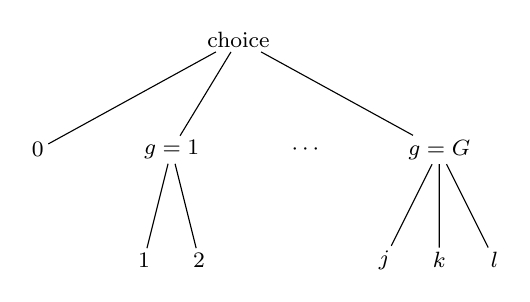
\begin{tikzpicture}[font=\footnotesize, level distance=14mm,
  level 1/.style={sibling distance=17mm}, level 2/.style={sibling distance=7mm},
  every node/.style={inner sep=1.5pt}]
\node (root) {choice}
  child {node {$0$}}
  child {node {$g = 1$}
    child {node {$1$}}
    child {node {$2$}}}
  child {node {$\cdots$} edge from parent[draw=none]}
  child {node {$g = G$}
    child {node {$j$}}
    child {node {$k$}}
    child {node {$l$}}};
\end{tikzpicture}
\caption{One level}
\end{subfigure}\hfill
\begin{subfigure}[b]{0.49\textwidth}
\centering
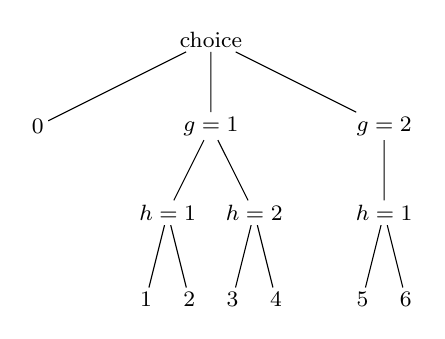
\begin{tikzpicture}[font=\footnotesize, level distance=11mm,
  level 1/.style={sibling distance=22mm}, level 2/.style={sibling distance=11mm},
  level 3/.style={sibling distance=5.5mm},
  every node/.style={inner sep=1.5pt}]
\node {choice}
  child {node {$0$}}
  child {node {$g = 1$}
    child {node {$h = 1$}
      child {node {$1$}}
      child {node {$2$}}}
    child {node {$h = 2$}
      child {node {$3$}}
      child {node {$4$}}}}
  child {node {$g = 2$}
    child {node {$h = 1$}
      child {node {$5$}}
      child {node {$6$}}}};
\end{tikzpicture}
\caption{Two levels}
\end{subfigure}
\caption{Nesting trees. In panel (a) the outside good $0$ is alone in its nest and the inside products are grouped
into nests $g = 1, \dots, G$. The nest choice is a logit in the inclusive values $I_g = (1-\sigma)\ln D_g$, and the
choice within a nest is a logit with scale $1 - \sigma$. In panel (b) each group $g$ is split into subgroups $h$,
with within-subgroup parameter $\sigma_1$ and within-group parameter $\sigma_2 \le \sigma_1$.}
\label{fig:07-nl-tree}
\end{figure}

\subsection{Substitution patterns}\label{sec:07-nl-substitution}

All substitution patterns follow from one derivative. Taking logs in \eqref{eq:07-nl-share},
\begin{align*}
\ln s_j &= \ln s_{j \mid g} + \ln s_g \\
&= \frac{\delta_j}{1-\sigma} - \ln D_g + (1-\sigma)\ln D_g - \ln\Big(1 + \sum_h D_h^{1-\sigma}\Big) \\
&= \frac{\delta_j}{1-\sigma} - \sigma\ln D_g - \ln\Big(1 + \sum_h D_h^{1-\sigma}\Big) .
\end{align*}
Differentiate each term with respect to $\delta_k$. The first term gives $\frac{\indic\{j = k\}}{1-\sigma}$. For the
second, $\frac{\partial \ln D_g}{\partial \delta_k} = \frac{1}{1-\sigma}s_{k \mid g}$ if $k \in g$ and zero otherwise.
For the third, if $k$ belongs to nest $h$,
\begin{equation*}
\frac{\partial}{\partial \delta_k}\ln\Big(1 + \sum_{h'} D_{h'}^{1-\sigma}\Big)
= \frac{(1-\sigma)D_h^{-\sigma}\cdot\frac{1}{1-\sigma}e^{\frac{\delta_k}{1-\sigma}}}{1 + \sum_{h'}D_{h'}^{1-\sigma}}
= s_{k \mid h}\,s_h = s_k .
\end{equation*}
Collecting terms,
\begin{equation}\label{eq:07-nl-dlns}
\frac{\partial \ln s_j}{\partial \delta_k} = \frac{\indic\{j = k\}}{1-\sigma} - \frac{\sigma}{1-\sigma}\,s_{k \mid g}\,\indic\{k \in g\} - s_k ,
\qquad j \in g .
\end{equation}
The same expression follows from \eqref{eq:07-gev-deriv} with the generating function \eqref{eq:07-nl-H}. Since
$\frac{\partial \delta_k}{\partial p_k} = -\alpha$, the price derivatives are
\begin{align}
\frac{\partial s_j}{\partial p_j} &= -\alpha s_j\Big[\frac{1}{1-\sigma} - \frac{\sigma}{1-\sigma}s_{j \mid g} - s_j\Big], \label{eq:07-nl-own}\\
\frac{\partial s_j}{\partial p_k} &= \alpha s_j\Big[\frac{\sigma}{1-\sigma}s_{k \mid g} + s_k\Big], \qquad k \in g,\; k \neq j, \label{eq:07-nl-cross-in}\\
\frac{\partial s_j}{\partial p_k} &= \alpha s_j s_k, \qquad k \notin g . \label{eq:07-nl-cross-out}
\end{align}
The bracket in \eqref{eq:07-nl-own} equals $\frac{1 - \sigma s_{j \mid g} - (1-\sigma)s_j}{1-\sigma}$, which is positive
because $s_{j \mid g} \le 1$ and $s_j < 1$. Multiplying by $\frac{p_j}{s_j}$ or $\frac{p_k}{s_j}$ gives the elasticities.
With the own elasticity written as a positive number,
\begin{equation}\label{eq:07-nl-elast}
\varepsilon_j = \alpha p_j\Big[\frac{1}{1-\sigma} - \frac{\sigma}{1-\sigma}s_{j \mid g} - s_j\Big], \qquad
\varepsilon_{jk} =
\begin{cases}
\alpha p_k\Big[\frac{\sigma}{1-\sigma}s_{k \mid g} + s_k\Big], & k \in g, \\[4pt]
\alpha p_k s_k, & k \notin g .
\end{cases}
\end{equation}

These formulas have four implications.
\begin{enumerate}[label=(\alph*)]
  \item Within a nest, substitution is proportional to shares. The cross elasticity $\varepsilon_{jk}$ for
  $k \in g$ depends on $k$ alone, so a rise in $p_k$ raises the shares of all of $k$'s nest-mates in the same
  proportion. Equivalently, $\frac{s_j}{s_l} = e^{\frac{\delta_j - \delta_l}{1-\sigma}}$ for $j, l \in g$, so IIA holds
  within each nest.
  \item Across nests, substitution is also proportional to shares. A rise in $p_k$ raises the shares of all
  products outside $k$'s nest, and of the outside good, by the same proportion $\alpha s_k\,\dd p_k$, exactly as in
  the logit.
  \item The same-nest cross elasticity exceeds the cross elasticity for products in other nests by
  $\alpha p_k\frac{\sigma}{1-\sigma}s_{k \mid g}$. This is the extra substitution among similar products that the
  logit lacks.
  \item IIA fails between products in different nests. For $j \in g$ and $l \in h \neq g$,
  $\frac{s_j}{s_l} = e^{\frac{\delta_j - \delta_l}{1-\sigma}}\big(\frac{D_h}{D_g}\big)^{\sigma}$ depends on every product of
  the two nests.
\end{enumerate}
The own elasticity keeps the main defect of the logit. For small shares it is close to
$\frac{\alpha p_j}{1-\sigma}(1 - \sigma s_{j \mid g})$, which rises almost in proportion to price. As
\citet[p.~524]{Nevo2000a} puts it, the nested logit ``does not help with the problem of own-price elasticities''.

\casehead{Diversion ratios}
Recall from \cref{sec:07-logit-elasticities} that the diversion ratio $D_{jk} = -\frac{\partial s_k}{\partial
p_j}\big(\frac{\partial s_j}{\partial p_j}\big)^{-1}$ is the fraction of the sales that $j$ loses after a small price
increase that go to $k$. For $k$ in the same nest as $j$,
\eqref{eq:07-nl-cross-in} with the roles of $j$ and $k$ exchanged gives
$\frac{\partial s_k}{\partial p_j} = \alpha s_k\big[\frac{\sigma}{1-\sigma}s_{j \mid g} + s_j\big]$. Because
$s_ks_{j \mid g} = s_{k \mid g}s_gs_{j \mid g} = s_js_{k \mid g}$, this equals
$\alpha s_j\big[\frac{\sigma}{1-\sigma}s_{k \mid g} + s_k\big]$. Dividing by minus \eqref{eq:07-nl-own} and multiplying
numerator and denominator by $1 - \sigma$,
\begin{equation}\label{eq:07-nl-diversion}
D_{jk} =
\begin{cases}
\frac{\sigma s_{k \mid g} + (1-\sigma)s_k}{1 - \sigma s_{j \mid g} - (1-\sigma)s_j}, & k \in g, \\[6pt]
\frac{(1-\sigma)s_k}{1 - \sigma s_{j \mid g} - (1-\sigma)s_j}, & k \notin g .
\end{cases}
\end{equation}
The diversion to the outside good, $D_{j0}$, has the second form with $s_0$ in place of $s_k$. The ratios sum to one.
Summing the numerators over $k \in g$ with $k \neq j$, over the other nests, and over the outside good gives
\begin{equation*}
\sigma(1 - s_{j \mid g}) + (1-\sigma)(1 - s_j) = 1 - \sigma s_{j \mid g} - (1-\sigma)s_j ,
\end{equation*}
which is the denominator. At $\sigma = 0$ every ratio reduces to the logit value $\frac{s_k}{1-s_j}$. Now let
$\sigma \to 1$ with the shares held fixed and $s_{j \mid g} < 1$. Then all diversion stays within the nest, in
proportion to within-nest shares. The condition on $s_{j \mid g}$ matters. Writing the denominator as
$\sigma(1 - s_{j \mid g}) + (1-\sigma)(1 - s_j)$,
\begin{equation*}
D_{j0} = \frac{(1-\sigma)s_0}{\sigma(1 - s_{j \mid g}) + (1-\sigma)(1 - s_j)} ,
\end{equation*}
which vanishes only if $\frac{1 - s_{j \mid g}}{1-\sigma}$ grows without bound. A product alone in its nest has
$s_{j \mid g} = 1$, so $D_{j0} = \frac{s_0}{1 - s_j}$ for every $\sigma$. The limit also fails when mean utilities,
rather than shares, are held fixed and $j$ is the unique best product in its nest. Then $1 - s_{j \mid g}$ falls
exponentially in $\frac{1}{1-\sigma}$, and $D_{j0}$ tends to $\frac{s_0}{1 - s_j}$ at the limiting shares.
\Cref{tab:07-nl-formulas} collects the formulas of this section and the next three subsections.

\begin{table}[htbp]
\centering
\caption{Logit and nested logit formulas}\label{tab:07-nl-formulas}
\small
\renewcommand{\arraystretch}{1.8}
\begin{tabular}{@{}lll@{}}
\toprule
Object & Logit & Nested logit ($j \in g$) \\
\midrule
Share $s_j$ & $\displaystyle \frac{e^{\delta_j}}{1 + \sum_k e^{\delta_k}}$ & $\displaystyle \frac{e^{\frac{\delta_j}{1-\sigma}}}{D_g^{\sigma}\left(1 + \sum_h D_h^{1-\sigma}\right)}$ \\
Inversion & $\displaystyle \delta_j = \ln s_j - \ln s_0$ & $\displaystyle \delta_j = \ln s_j - \ln s_0 - \sigma\ln s_{j \mid g}$ \\
Own elasticity $\varepsilon_j$ & $\displaystyle \alpha p_j(1 - s_j)$ & $\displaystyle \alpha p_j\left[\frac{1}{1-\sigma} - \frac{\sigma}{1-\sigma}s_{j \mid g} - s_j\right]$ \\
Cross elasticity, $k \in g$ & $\displaystyle \alpha p_k s_k$ & $\displaystyle \alpha p_k\left[\frac{\sigma}{1-\sigma}s_{k \mid g} + s_k\right]$ \\
Cross elasticity, $k \notin g$ & $\displaystyle \alpha p_k s_k$ & $\displaystyle \alpha p_k s_k$ \\
Diversion $D_{jk}$, $k \in g$ & $\displaystyle \frac{s_k}{1 - s_j}$ & $\displaystyle \frac{\sigma s_{k \mid g} + (1-\sigma)s_k}{1 - \sigma s_{j \mid g} - (1-\sigma)s_j}$ \\
Diversion $D_{jk}$, $k \notin g$ or $k = 0$ & $\displaystyle \frac{s_k}{1 - s_j}$ & $\displaystyle \frac{(1-\sigma)s_k}{1 - \sigma s_{j \mid g} - (1-\sigma)s_j}$ \\
Single-product markup & $\displaystyle \frac{1}{\alpha(1 - s_j)}$ & $\displaystyle \frac{1-\sigma}{\alpha\left[1 - \sigma s_{j \mid g} - (1-\sigma)s_j\right]}$ \\
Multi-product markup & $\displaystyle \frac{1}{\alpha(1 - S_f)}$ & $\displaystyle \frac{1-\sigma}{\alpha(1 - \sigma S_{f \mid g})(1 - \Phi_f)}$ \\
Consumer surplus, up to $C$ & $\displaystyle \frac{1}{\alpha}\ln\left(1 + \sum_k e^{\delta_k}\right)$ & $\displaystyle \frac{1}{\alpha}\ln\left(1 + \sum_h D_h^{1-\sigma}\right)$ \\
Removing $j$, change in $CS$ & $\displaystyle \frac{1}{\alpha}\ln(1 - s_j)$ & $\displaystyle \frac{1}{\alpha}\ln\left[1 - s_g + s_g(1 - s_{j \mid g})^{1-\sigma}\right]$ \\
\bottomrule
\end{tabular}
\par\smallskip
\begin{minipage}{0.95\textwidth}
\footnotesize Notes: $D_g = \sum_{k \in g}e^{\frac{\delta_k}{1-\sigma}}$, $s_{j \mid g} = \frac{s_j}{s_g}$, and
$\delta_j = x_j\beta - \alpha p_j + \xi_j$. Own elasticities are positive numbers. $S_f$ is the combined share
of firm $f$, $S_{f \mid g}$ its share within nest $g$, and
$\Phi_f = \sum_h \frac{(1-\sigma)S_{fh}}{1 - \sigma S_{f \mid h}}$ (\cref{prop:07-nl-multi}). Welfare formulas are per
consumer, at fixed prices, with the outside good alone in its nest (\cref{prop:07-logsum,cor:07-removal}).
\end{minipage}
\end{table}

\casehead{Red bus, blue bus}
The classic example shows what nesting achieves (\cref{sec:07-iia}). A commuter chooses between a car and a red
bus with equal mean utilities, so each has share $\frac{1}{2}$. A blue bus identical to the red bus is added.
Place the car alone in one nest and the two buses in another, and normalize the car's mean utility to zero, as for
an outside good. With bus mean utility $\delta = 0$, the bus nest has $D_{\text{bus}} = 2$ and
$D_{\text{bus}}^{1-\sigma} = 2^{1-\sigma}$. By \eqref{eq:07-nl-share},
\begin{equation}\label{eq:07-redbus}
s_{\text{car}} = \frac{1}{1 + 2^{1-\sigma}}, \qquad
s_{\text{red}} = s_{\text{blue}} = \frac{1}{2}\cdot\frac{2^{1-\sigma}}{1 + 2^{1-\sigma}} = \frac{2^{-\sigma}}{1 + 2^{1-\sigma}} .
\end{equation}
At $\sigma = 0$ every mode has share $\frac{1}{3}$, the logit answer. At $\sigma = 0.5$ the car keeps $0.414$ and
each bus has $0.293$. As $\sigma \to 1$ the shares approach $\big(\frac{1}{2}, \frac{1}{4}, \frac{1}{4}\big)$,
the commonsense answer. \Cref{fig:07-redbus} plots the three shares against $\sigma$. The nested logit resolves the
paradox only because the analyst put the two buses in the same nest.

\begin{figure}[htbp]
\centering
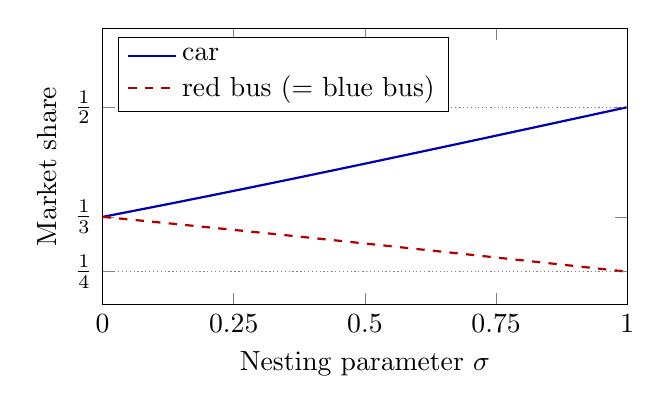
\begin{tikzpicture}
\begin{axis}[width=0.68\textwidth, height=0.42\textwidth,
  xlabel={Nesting parameter $\sigma$}, ylabel={Market share},
  xmin=0, xmax=1, ymin=0.2, ymax=0.62,
  ytick={0.25,0.3333,0.5}, yticklabels={$\frac{1}{4}$,$\frac{1}{3}$,$\frac{1}{2}$},
  xtick={0,0.25,0.5,0.75,1},
  domain=0:0.999, samples=120, legend style={at={(0.03,0.97)}, anchor=north west}, legend cell align=left,
  every axis plot/.append style={thick}]
\addplot[blue!70!black] {1/(1+2^(1-x))};
\addlegendentry{car}
\addplot[red!70!black, dashed] {2^(-x)/(1+2^(1-x))};
\addlegendentry{red bus (= blue bus)}
\addplot[gray, thin, densely dotted, domain=0:1] {0.5};
\addplot[gray, thin, densely dotted, domain=0:1] {0.25};
\end{axis}
\end{tikzpicture}
\caption{Red bus, blue bus. Shares of the car and of each bus from \eqref{eq:07-redbus} when the two buses form one
nest and the car is alone in its nest, all with equal mean utilities. The logit ($\sigma = 0$) gives
$\frac{1}{3}$ to each mode. As $\sigma \to 1$ the car keeps $\frac{1}{2}$ and the buses split the other half.}
\label{fig:07-redbus}
\end{figure}

\subsection{Estimation}\label{sec:07-nl-estimation}

Like the logit, the nested logit can be inverted in closed form, and the inverted equation is linear in the
parameters.

\begin{proposition}[Nested logit inversion]\label{prop:07-nl-inversion}
Under \cref{asm:07-nl}, let the observed shares $s_j > 0$ and $s_0 > 0$ sum to one. Let
$\bar s_g = \sum_{k\in g}s_k$ be the observed nest shares and $s_{j \mid g} = \frac{s_j}{\bar s_g}$ the observed
within-nest shares. For a given $\sigma \in [0, 1)$, the unique mean utilities that reproduce the observed shares
are
\begin{equation}\label{eq:07-nl-delta}
\delta_j = \ln s_j - \ln s_0 - \sigma\ln s_{j \mid g} .
\end{equation}
With $\delta_{jt} = x_{jt}\beta - \alpha p_{jt} + \xi_{jt}$ in market $t$, the shares satisfy
\begin{equation}\label{eq:07-nl-regression}
\ln s_{jt} - \ln s_{0t} = x_{jt}\beta - \alpha p_{jt} + \sigma\ln s_{j \mid g, t} + \xi_{jt} .
\end{equation}
\end{proposition}

\begin{proof}
Start from the expression for $\ln s_j$ derived before \eqref{eq:07-nl-dlns} and subtract
$\ln s_0 = -\ln(1 + \sum_h D_h^{1-\sigma})$:
\begin{equation*}
\ln s_j - \ln s_0 = \frac{\delta_j}{1-\sigma} - \sigma\ln D_g .
\end{equation*}
This still contains the unobserved inclusive sum. The within-nest share gives
$\ln s_{j \mid g} = \frac{\delta_j}{1-\sigma} - \ln D_g$, so
$\ln D_g = \frac{\delta_j}{1-\sigma} - \ln s_{j \mid g}$. Substituting,
\begin{align*}
\ln s_j - \ln s_0 &= \frac{\delta_j}{1-\sigma} - \frac{\sigma\delta_j}{1-\sigma} + \sigma\ln s_{j \mid g} \\
&= \delta_j + \sigma\ln s_{j \mid g} ,
\end{align*}
which rearranges to \eqref{eq:07-nl-delta}. Any $\delta$ that reproduces the shares must therefore equal
\eqref{eq:07-nl-delta}.

To show that \eqref{eq:07-nl-delta} reproduces the shares, compute its inclusive sums. Using
$s_k = \bar s_g s_{k \mid g}$,
\begin{equation*}
e^{\frac{\delta_k}{1-\sigma}} = \Big(\frac{s_k}{s_0}\Big)^{\frac{1}{1-\sigma}}s_{k \mid g}^{-\frac{\sigma}{1-\sigma}}
= \Big(\frac{\bar s_g}{s_0}\Big)^{\frac{1}{1-\sigma}}s_{k \mid g} .
\end{equation*}
Summing over $k \in g$ gives $D_g = \big(\frac{\bar s_g}{s_0}\big)^{\frac{1}{1-\sigma}}$, so
$D_g^{1-\sigma} = \frac{\bar s_g}{s_0}$. The model's within-nest share is then
$\frac{e^{\frac{\delta_j}{1-\sigma}}}{D_g} = s_{j \mid g}$. Its nest share is
$\frac{\bar s_g s_0^{-1}}{1 + \sum_h \bar s_h s_0^{-1}} = \frac{\bar s_g}{s_0 + \sum_h \bar s_h} = \bar s_g$, because the
shares sum to one. Both factors match the data, so the model reproduces every $s_j$.
\end{proof}

\citet[eqs.~26--28, p.~253]{Berry1994} reaches the same equation by eliminating $D_g$ through the nest share,
$D_g^{1-\sigma} = \frac{\bar s_g}{s_0}$, the identity used in the second half of the proof
(\cref{sec:07-berry-examples} follows his route). The regression \eqref{eq:07-nl-regression} is the logit
regression \eqref{eq:07-logit-inversion} with one additional regressor, the log within-nest share. Its coefficient is the nesting parameter. \citet[n.~7]{Berry1994} notes that
the formula extends, ``easily (but somewhat tediously)'', to several levels of nests and to nest-specific
parameters $\sigma_g$. \Cref{sec:07-nl-twolevel} carries out the two-level case.

\casehead{One inside nest}
The cheapest nesting puts all inside goods in one nest and the outside good in the other. Then
$s_{j \mid g} = \frac{s_j}{1 - s_0}$, and \eqref{eq:07-nl-regression} becomes
\begin{equation}\label{eq:07-nl-onenest}
\ln s_{jt} - \ln s_{0t} = x_{jt}\beta - \alpha p_{jt} + \sigma\ln\frac{s_{jt}}{1 - s_{0t}} + \xi_{jt} .
\end{equation}
The model requires no classification of products, so it is often run as a robustness check on the logit. With one
inside nest and inclusive sum $D$, the share formula is
\begin{equation*}
s_j = \frac{e^{\frac{\delta_j}{1-\sigma}}D^{-\sigma}}{1 + D^{1-\sigma}} = \frac{e^{\frac{\delta_j}{1-\sigma}}}{D^{\sigma} + D} ,
\end{equation*}
which is the form \citet[eq.~3]{Einav2007} uses for movies (\cref{sec:07-einav}).

The nesting parameter then measures how much additional products expand the category rather than steal
business from rivals. Suppose the market has $J$ identical inside products with mean utility $\delta$. The total
inside share is $1 - s_0 = \frac{J^{1-\sigma}e^{\delta}}{1 + J^{1-\sigma}e^{\delta}}$, whose elasticity with respect to $J$
is $(1-\sigma)s_0$. At $\sigma = 0$ each new product draws consumers from the outside good as in the logit. As
$\sigma \to 1$ new copies only divide a fixed category. Raising the mean utility $\delta_j$ of an existing product is different. At given shares,
$\frac{\partial\ln(1 - s_0)}{\partial\delta_j} = s_0 s_{j \mid g}$ for every $\sigma$, which is the logit value
$\frac{s_0 s_j}{1 - s_0}$. A uniform rise $\Delta$ in all inside prices multiplies
$D^{1-\sigma}$ by $e^{-\alpha\Delta}$, so
\begin{equation*}
\frac{\dd\ln(1 - s_0)}{\dd\Delta} = -\alpha s_0 ,
\end{equation*}
the same as in the logit. For a given price coefficient, $\sigma$ leaves the category response unchanged. It raises
the own elasticity of a product with a small within-nest share by a factor close to $\frac{1}{1-\sigma}$.
\Citet[p.~1774]{MillerWeinberg2017} use the one-nest model for beer. Their richer specifications add random
coefficients that interact consumer income with price and product characteristics (Table~IV). They note that the nesting parameter keeps the elasticities from being overly sensitive to the
assumed market size (\cref{sec:07-market-size,ch:mergers}).

\casehead{Endogeneity of the within-nest share}
The within-nest share depends on $\xi_{jt}$. From \eqref{eq:07-nl-share},
$\frac{\partial\ln s_{j \mid g}}{\partial\xi_j} = \frac{1 - s_{j \mid g}}{1-\sigma} > 0$, so the regressor
$\ln s_{j \mid g, t}$ is positively correlated with the error. A high-quality product also lowers the within-nest
shares of its nest-mates, so the regressor is endogenous for every product in the nest. OLS therefore tends to
bias $\hat\sigma$ upward, toward one. Prices are endogenous as in the logit (\cref{sec:07-endogeneity}). Estimating
\eqref{eq:07-nl-regression} needs at least two excluded instruments, one for $p_{jt}$ and one for
$\ln s_{j \mid g, t}$, and the two must move the regressors in different ways.

Instruments for the within-nest share shift the crowding of a product's nest without shifting its own unobserved
quality. Common choices follow.
\begin{itemize}
  \item The number of products in the nest, $J_{gt}$. More nest-mates lower $s_{j \mid g}$ mechanically.
  \item Sums or averages of the characteristics of the other products in the nest. \citet[p.~254]{Berry1994}
  suggests ``the characteristics of other firms in the group''. These are the nest-level versions of the BLP
  instruments of \cref{sec:07-instruments}, and the differentiation instruments of \citet{GandhiHoude2019}
  refine them.
  \item Cost shifters of the other products in the nest, which move their prices and hence $s_{j \mid g}$.
  \item Application-specific counts. \citet{Einav2007} uses the number of movies showing in the same week.
\end{itemize}
These instruments are valid if the number and characteristics of nest-mates are mean independent of $\xi_{jt}$.
Endogenous entry threatens this condition. Firms add products to nests and markets where demand is high, so
$J_{gt}$ may be correlated with $\xi_{jt}$. Product and market fixed effects absorb persistent demand differences
and reduce the concern, provided entry does not respond to transitory shocks.

\casehead{What identifies $\sigma$}
Fix a product's mean utility and add a rival to its nest. The rival lowers $\ln s_{j \mid g}$. By
\eqref{eq:07-nl-regression}, it lowers $\ln\frac{s_j}{s_0}$ by $\sigma$ times as much. A rival added to a different
nest changes neither the within share nor the ratio $\frac{s_j}{s_0}$. With $\sigma = 0$ the ratio $\frac{s_j}{s_0}$ does not respond at all, which is IIA. With
$\sigma$ near one it falls almost one for one with the within share. A rival that does not beat the best product in
the nest then steals customers almost only from its nest-mates. A better rival also draws from the outside good,
because it raises the nest's best mean utility. Comparing the same product across markets with exogenously different nest-mates therefore traces out
$\sigma$. On the supply side, \citet[pp.~255--256]{Berry1994} adds that the joint behavior of prices, product shares
and group shares in the pricing equation helps identify $\sigma$ (\cref{sec:07-nl-pricing}). Estimates of
$\sigma$ outside $[0, 1)$ signal a misspecified tree or invalid instruments (\cref{lem:07-nl-gev}).

\casehead{Estimation from individual choices}
With data on individual choices, the nested logit can be estimated by maximum likelihood, as the logit is in
\cref{sec:07-micro-ml}. Let consumer $i$ have utility index $V_{ij}$ in place of $\delta_j$, with the outside good
normalized to zero. For $j$ in nest $g$, split the index into a part $z_{ig}\gamma$ that is constant within the nest
and a part $w_{ij}b$ that varies within it, $V_{ij} = z_{ig}\gamma + w_{ij}b$. The inclusive sum
$D_{ig} = \sum_{k \in g}e^{\frac{V_{ik}}{1-\sigma}}$ then satisfies
\begin{equation*}
\ln D_{ig} = \frac{z_{ig}\gamma}{1-\sigma} + I_{ig}, \qquad
I_{ig} = \ln\sum_{k \in g}\exp\Big(\frac{w_{ik}b}{1-\sigma}\Big) .
\end{equation*}
Substituting into \cref{prop:07-nl-shares}, the choice probability factors into a within-nest and a nest
probability,
\begin{equation}\label{eq:07-nl-sequential}
P_{ij \mid g} = \exp\Big(\frac{w_{ij}b}{1-\sigma} - I_{ig}\Big), \qquad
P_{ig} = \frac{\exp\big(z_{ig}\gamma + (1-\sigma)I_{ig}\big)}{1 + \sum_h\exp\big(z_{ih}\gamma + (1-\sigma)I_{ih}\big)} .
\end{equation}
The log-likelihood sums $\ln P_{ij \mid g} + \ln P_{ig}$ over the observed choices. Unlike the logit likelihood of
\cref{prop:07-ml-concave}, it ``is not concave in all parameters, and is highly non-linear in the inclusive value
coefficients'' \citep[p.~1426]{McFadden1984}. A search can then stop at a local maximum, so it should start from
several points.

\Cref{eq:07-nl-sequential} suggests a \emph{sequential estimator}. The first step fits a logit to the choices within
each nest, which estimates $\frac{b}{1-\sigma}$. The second step computes the estimated inclusive values $\hat I_{ig}$
and fits a logit to the choice of nest, with regressors $z_{ig}$ and $\hat I_{ig}$. The coefficient on $\hat I_{ig}$
estimates $1 - \sigma$. Each step is a concave logit problem. McFadden notes that the estimator is consistent but
often inefficient. Its second-step standard errors are wrong, because the inclusive values are estimated, and
correction formulae exist (p.~1426). One Newton step on the full likelihood from the sequential estimates is
asymptotically equivalent to full maximum likelihood. In practice the strong nonlinearity can make this one-step
estimator erratic, so several iterations may be needed. In McFadden's housing example (\cref{tab:07-mcfadden-housing})
only \textit{OPCOST} and \textit{YNH} vary among renters, so only their coefficients enter the first step. There the
two estimators agree to the third decimal place, with log-likelihoods of $-10.7868$ for the sequential estimates and
$-10.7862$ at the full maximum (p.~1432).

\casehead{Choosing the nests}
The nests must be fixed before estimation, a limitation the nested logit shares with multi-stage budgeting
(\cref{ch:aids}). The classification is often unclear. Is a minivan a car or a truck? Are store-brand and
national-brand cereals in the same nest? Is a family sedan closer to a compact car or to a luxury car? Different
nestings imply different substitution patterns, and the data may not discriminate between them. With several
levels the order of the nests also matters. \citet[n.~18]{Nevo2000a} notes that classifying computers first into
branded and unbranded and then into frontier and non-frontier technology implies different substitution than the
reverse order, even with the same classification. Practical checks include estimating nest-specific parameters
$\sigma_g$, comparing non-nested trees by fit, and checking that all estimates lie in $[0, 1)$.

\casehead{A Monte Carlo experiment}
We illustrate these points with a simulation. Each sample has $500$ markets with two inside nests and an outside
good. In the main design the number of products in each nest is drawn uniformly from $\{1, \dots, 5\}$ in every
market. Each product has its own owner. Mean utility is $\delta_j = \beta_0 + \beta_xx_j - \alpha p_j + \xi_j$ with
$\beta_0 = 2$, $\beta_x = 1$, $\alpha = 1$ and $\sigma = 0.5$. Marginal cost is
$c_j = \exp(0.5 + 0.25x_j + 0.25w_j + 0.1\xi_j + 0.25\omega_j)$, where $x_j$, $\xi_j$, $w_j$ and $\omega_j$
are independent standard normal variables. Prices are the single-product Bertrand-Nash equilibrium of
\cref{prop:07-nl-markup}. The average outside share is $0.28$ and the average within-nest share is $0.33$. There
are five excluded instruments. The first two are the own cost shifter $w_j$ and the number of products in the own
nest. The other three are sums over rival products. They add up $x$ over the other products in the own nest, $x$
over the products of the other nest, and $w$ over the other products in the own nest. We draw $500$ samples. A second design fixes three products in every nest, so the count
instrument disappears.

\begin{table}[htbp]
\centering
\caption{Monte Carlo estimates of the nested logit regression}\label{tab:07-mc-nl}
\small
\begin{tabular}{@{}lcccccc@{}}
\toprule
 & & \multicolumn{4}{c}{Nest sizes vary across markets} & Fixed size \\
\cmidrule(lr){3-6}\cmidrule(lr){7-7}
Parameter & True & OLS & IV, price only & IV, both & Logit IV & IV, both \\
\midrule
$\beta_0$ & 2.0 & 0.920 & 2.258 & 2.003 & 1.561 & 1.997 \\
 & & (0.055) & (0.120) & (0.115) & (0.204) & (0.121) \\
$\beta_x$ & 1.0 & 0.462 & 0.760 & 1.001 & 1.417 & 0.998 \\
 & & (0.022) & (0.036) & (0.034) & (0.053) & (0.047) \\
$\alpha$ & 1.0 & 0.334 & 0.870 & 1.002 & 1.228 & 0.998 \\
 & & (0.022) & (0.049) & (0.045) & (0.082) & (0.057) \\
$\sigma$ & 0.5 & 0.801 & 0.787 & 0.499 & 0 & 0.500 \\
 & & (0.009) & (0.010) & (0.019) &  & (0.031) \\
\addlinespace
Mean own elasticity & 3.83 & 2.91 & 7.16 & 3.83 & 2.71 & 3.83 \\
 & & (0.19) & (0.40) & (0.19) & (0.18) & (0.20) \\
\bottomrule
\end{tabular}
\par\smallskip
\begin{minipage}{0.95\textwidth}
\footnotesize Notes: Means across 500 simulated samples of 500 markets, with standard deviations across samples
in parentheses. Columns 3 to 6 use the main design, in which each of the two nests has between one and five
products. Column 7 fixes three products per nest. ``IV, price only'' instruments the price and treats
$\ln s_{j \mid g}$ as exogenous. ``IV, both'' instruments both. ``Logit IV'' imposes $\sigma = 0$. The mean own
elasticity averages $\varepsilon_j$ from \eqref{eq:07-nl-elast} over products at the estimated parameters. Its
true value is $3.83$ in the main design and $3.82$ in the fixed-size design. Mean first-stage $F$ statistics of
the excluded instruments are $304$ for price and $277$ for $\ln s_{j \mid g}$ in the main design, and $336$ and
$183$ in the fixed-size design. Computed by \texttt{figures/ch07/src/mc\_nested\_logit.py}.
\end{minipage}
\end{table}

\Cref{tab:07-mc-nl} reports the results. OLS gives $\hat\sigma = 0.801$ against a true value of $0.5$ and cuts
the price coefficient to a third of its true value. Instrumenting the price alone fixes most of the price bias,
with $\hat\alpha = 0.870$. The nesting parameter stays near $0.79$, however, and the implied own elasticity of
$7.16$ is almost twice the true value of $3.83$. Treating the within-nest share as exogenous is therefore costly
even with a valid price instrument. Instrumenting both regressors recovers every parameter. Imposing the logit
($\sigma = 0$) with the same instruments biases $\hat\alpha$ and $\hat\beta_x$ upward. It also understates the mean
own elasticity by about 29 percent, because the factor $\frac{1}{1-\sigma}$ is missing from the elasticity formula.
With fixed nest sizes, the characteristics of nest-mates still identify $\sigma$. The standard deviation of
$\hat\sigma$ rises from $0.019$ to $0.031$, which shows that variation in the number of products adds
information.

\subsection{Pricing with nested logit demand}\label{sec:07-nl-pricing}

The nested logit keeps the analytic markups of the logit. We first treat single-product firms and then derive a
closed form for multi-product firms.

\begin{proposition}[Single-product markups]\label{prop:07-nl-markup}
Under \cref{asm:07-nl} with constant marginal cost $mc_j$, the first-order condition of a single-product firm
selling $j \in g$ implies
\begin{equation}\label{eq:07-nl-markup}
p_j - mc_j = \frac{1-\sigma}{\alpha\big[1 - \sigma s_{j \mid g} - (1-\sigma)s_j\big]} .
\end{equation}
\end{proposition}

\begin{proof}
The firm maximizes $M(p_j - mc_j)s_j(p)$. The first-order condition is
$s_j + (p_j - mc_j)\frac{\partial s_j}{\partial p_j} = 0$. By \eqref{eq:07-nl-own},
\begin{equation*}
\frac{\partial s_j}{\partial p_j} = -\frac{\alpha s_j}{1-\sigma}\big[1 - \sigma s_{j \mid g} - (1-\sigma)s_j\big] .
\end{equation*}
Substituting and dividing by $s_j > 0$,
\begin{equation*}
1 - \frac{\alpha(p_j - mc_j)}{1-\sigma}\big[1 - \sigma s_{j \mid g} - (1-\sigma)s_j\big] = 0 ,
\end{equation*}
which rearranges to \eqref{eq:07-nl-markup}.
\end{proof}

This is equation (33) of \citet[p.~255]{Berry1994}. With $mc_j = w_j\gamma + \omega_j$ it becomes a linear supply
equation, $p_j = w_j\gamma + \frac{1-\sigma}{\alpha[1 - \sigma s_{j \mid g} - (1-\sigma)s_j]} + \omega_j$, which can be
estimated jointly with \eqref{eq:07-nl-regression} as in \cref{sec:07-cost-recovery}. When $\sigma = 0$ only the
product share matters, as in the logit markup $\frac{1}{\alpha(1-s_j)}$. As $\sigma \to 1$ with $s_{j \mid g} < 1$
held fixed, only the within-nest share matters. A product alone in its nest keeps the logit markup for every
$\sigma$. The markup is at least $\frac{1-\sigma}{\alpha}$, so the logit floor $\frac{1}{\alpha}$ falls as products become
closer substitutes. If $\sigma \to 1$ and a nest holds many products with small within shares, the markup goes to
zero, which is Bertrand competition with perfect substitutes.

\begin{proposition}[Multi-product markups]\label{prop:07-nl-multi}
Under \cref{asm:07-nl} with constant marginal costs, let firm $f$ own the products $\mathcal{J}_f$. Write
$S_{fh} = \sum_{k \in \mathcal{J}_f \cap h}s_k$ for its combined share in nest $h$ and
$S_{f \mid h} = \frac{S_{fh}}{s_h}$ for its share within nest $h$. At an interior Bertrand-Nash equilibrium, all of
the firm's products in a nest $g$ carry the same markup,
\begin{equation}\label{eq:07-nl-multi}
m_{fg} = \frac{1-\sigma}{\alpha\big(1 - \sigma S_{f \mid g}\big)\big(1 - \Phi_f\big)}, \qquad
\Phi_f = \sum_{h} \frac{(1-\sigma)S_{fh}}{1 - \sigma S_{f \mid h}} ,
\end{equation}
where the sum runs over the nests in which $f$ sells, and $0 \le \Phi_f < 1$.
\end{proposition}

\begin{proof}
Write $m_k = p_k - mc_k$. The firm maximizes $M\sum_{k\in\mathcal{J}_f}m_ks_k(p)$. The first-order condition for
$j \in \mathcal{J}_f \cap g$ is
\begin{equation*}
s_j + \sum_{k \in \mathcal{J}_f}m_k\frac{\partial s_k}{\partial p_j} = 0 .
\end{equation*}
By \eqref{eq:07-nl-dlns} with the roles of $j$ and $k$ exchanged, and $\frac{\partial\delta_j}{\partial p_j} = -\alpha$,
\begin{equation*}
\frac{\partial s_k}{\partial p_j} = -\alpha s_k\Big[\frac{\indic\{k = j\}}{1-\sigma} - \frac{\sigma}{1-\sigma}s_{j \mid g}\indic\{k \in g\} - s_j\Big] .
\end{equation*}
Substituting into the first-order condition,
\begin{equation*}
s_j - \frac{\alpha m_js_j}{1-\sigma} + \frac{\alpha\sigma}{1-\sigma}s_{j \mid g}\sum_{k\in\mathcal{J}_f\cap g}m_ks_k
+ \alpha s_j\sum_{k\in\mathcal{J}_f}m_ks_k = 0 .
\end{equation*}
Divide by $s_j$ and use $\frac{s_{j \mid g}}{s_j} = \frac{1}{s_g}$ and $\frac{s_k}{s_g} = s_{k \mid g}$. Multiplying by
$\frac{1-\sigma}{\alpha}$,
\begin{equation*}
m_j = \frac{1-\sigma}{\alpha} + \sigma\sum_{k\in\mathcal{J}_f\cap g}m_ks_{k \mid g} + (1-\sigma)\sum_{k\in\mathcal{J}_f}m_ks_k .
\end{equation*}
The right side depends on $j$ only through its nest $g$. Hence $m_j = m_{fg}$ for every
$j \in \mathcal{J}_f \cap g$. The first sum then equals $m_{fg}S_{f \mid g}$ and the second equals
$\sum_h m_{fh}S_{fh}$. Let $A_f = \frac{1-\sigma}{\alpha} + (1-\sigma)\sum_h m_{fh}S_{fh}$, which does not depend on
$g$. Then
\begin{equation*}
m_{fg}\big(1 - \sigma S_{f \mid g}\big) = A_f, \qquad\text{so}\qquad m_{fg} = \frac{A_f}{1 - \sigma S_{f \mid g}} .
\end{equation*}
Substituting back into the definition of $A_f$,
\begin{equation*}
A_f = \frac{1-\sigma}{\alpha} + A_f\sum_h\frac{(1-\sigma)S_{fh}}{1 - \sigma S_{f \mid h}} = \frac{1-\sigma}{\alpha} + A_f\Phi_f ,
\end{equation*}
so $A_f = \frac{1-\sigma}{\alpha(1 - \Phi_f)}$, which gives \eqref{eq:07-nl-multi}. For the bound, each term of
$\Phi_f$ equals $s_h\frac{(1-\sigma)S_{f \mid h}}{1 - \sigma S_{f \mid h}} \le s_h$, since $(1-\sigma)x \le 1 - \sigma x$ for
$x \le 1$. Hence $\Phi_f \le \sum_h s_h \le 1 - s_0 < 1$.
\end{proof}

Two checks confirm the formula. For a single product, $S_{f \mid g} = s_{j \mid g}$, $S_{fg} = s_j$ and
$\Phi_f = \frac{(1-\sigma)s_j}{1 - \sigma s_{j \mid g}}$. The product
$(1 - \sigma s_{j \mid g})(1 - \Phi_f)$ equals $1 - \sigma s_{j \mid g} - (1-\sigma)s_j$, which gives
\eqref{eq:07-nl-markup}. At $\sigma = 0$, $\Phi_f = \sum_h S_{fh} = S_f$ and $m_{fg} = \frac{1}{\alpha(1 - S_f)}$, the
logit result of \cref{prop:07-logit-multi}. The formula has two layers of internalized cannibalization. The
factor $1 - \sigma S_{f \mid g}$ captures recapture within the nest, which grows with $\sigma$ and with the firm's
within-nest share. The factor $1 - \Phi_f$ captures recapture across all of the firm's nests through the common
outside option.

\begin{example}[Ownership and markups]\label{ex:07-nl-markups}
Consider a market with two inside nests. Nest A has three products with shares $0.15$ each, nest B has two products
with shares $0.10$ each, and $s_0 = 0.35$. Let $\alpha = 1$. We compute the markup of a nest-A product implied by
\eqref{eq:07-nl-multi} at these observed shares, as one does when recovering costs from data.
\Cref{tab:07-nl-markup-example} reports three ownership structures. Under the logit, joint ownership of two nest-A
products raises the markup by 21.4 percent, and joint ownership of a nest-A and a nest-B product raises it by
13.3 percent. At $\sigma = 0.5$ the same changes raise it by 46.8 and 7.9 percent. At $\sigma = 0.8$ they raise it
by 73.0 and 3.6 percent. Common ownership matters far more within a nest than across nests once $\sigma$ is large.
The logit cannot make this distinction, which is why merger simulation with logit demand spreads price effects
evenly (\cref{ch:mergers}).
\end{example}

\begin{table}[htbp]
\centering
\caption{Implied markups of a nest-A product under alternative ownership}\label{tab:07-nl-markup-example}
\small
\begin{tabular}{@{}lccc@{}}
\toprule
Ownership & $\sigma = 0$ & $\sigma = 0.5$ & $\sigma = 0.8$ \\
\midrule
Single-product firms & 1.176 & 0.659 & 0.284 \\
One firm owns two nest-A products & 1.429 & 0.968 & 0.492 \\
One firm owns a nest-A and a nest-B product & 1.333 & 0.711 & 0.295 \\
\addlinespace
Percent increase, two nest-A products & 21.4 & 46.8 & 73.0 \\
Percent increase, nest-A and nest-B products & 13.3 & 7.9 & 3.6 \\
\bottomrule
\end{tabular}
\par\smallskip
\begin{minipage}{0.8\textwidth}
\footnotesize Notes: Illustrative shares $0.15$ for each of three nest-A products, $0.10$ for each of two nest-B
products, $s_0 = 0.35$, and $\alpha = 1$. Markups in dollars from \eqref{eq:07-nl-multi} at fixed shares. Computed by
\texttt{figures/ch07/src/nl\_markup\_example.py}.
\end{minipage}
\end{table}

The equilibrium can be computed in several ways. Iterating on the markup equation,
$p \leftarrow mc + m(p)$, is the simplest method. In our Monte Carlo experiment it settled into a two-cycle in some
markets with one dominant product. Iterating on exact best responses converged in every market of the experiment.
Each best response solves a one-dimensional equation, because the left side of the first-order condition
\eqref{eq:07-nl-markup} rises in the own price and the right side falls.

\subsection{The two-level nested logit}\label{sec:07-nl-twolevel}

Some markets have two natural dimensions of grouping. Cars differ by segment and by country of origin. Painkillers
differ by active substance and by form. The two-level nested logit, as used by \citet{Verboven1996}, splits each group $g$
into subgroups $h$ and adds a second nest taste. For product $j$ in subgroup $h$ of group $g$,
\begin{equation}\label{eq:07-nl2-utility}
u_{ij} = \delta_j + \zeta_{ig} + (1 - \sigma_2)\zeta_{ihg} + (1 - \sigma_1)\epsilon_{ij} ,
\end{equation}
with the outside good alone in its group. The parameter $\sigma_1$ measures the correlation of utilities within a
subgroup and $\sigma_2$ the correlation within a group.

The model is consistent with utility maximization when $0 \le \sigma_2 \le \sigma_1 < 1$. To see why, apply
\cref{lem:07-cardell} twice. Write the subgroup part of \eqref{eq:07-nl2-utility} as
\begin{equation*}
(1-\sigma_2)\Big[\zeta_{ihg} + \frac{1-\sigma_1}{1-\sigma_2}\epsilon_{ij}\Big] .
\end{equation*}
The bracket is Gumbel if $\zeta_{ihg} \sim C(\tau)$ with $1 - \tau = \frac{1-\sigma_1}{1-\sigma_2}$, which requires
$\tau \in [0, 1)$, that is $\sigma_1 \ge \sigma_2$. The group part, $\zeta_{ig}$ plus $1 - \sigma_2$
times a Gumbel variable, is then Gumbel if $\zeta_{ig} \sim C(\sigma_2)$.

The shares follow from the sequential derivation in the proof of \cref{prop:07-nl-shares}, applied level by level.
Within subgroup $hg$ the terms $\zeta_{ig}$ and $\zeta_{ihg}$ are common to all products, so the choice of product is
a logit with scale $1 - \sigma_1$. Let $D_{hg} = \sum_{k \in hg}e^{\frac{\delta_k}{1-\sigma_1}}$. By max-stability of
the Gumbel, the best utility in subgroup $hg$ is
\begin{equation*}
(1-\sigma_1)\ln D_{hg} + \zeta_{ig} + (1-\sigma_2)\Big[\zeta_{ihg} + \frac{1-\sigma_1}{1-\sigma_2}\tilde\epsilon_{ihg}\Big],
\end{equation*}
where $\tilde\epsilon_{ihg}$ is standard Gumbel. The bracket is standard Gumbel, as shown above, and $\zeta_{ig}$ is
common to all subgroups of $g$. So the choice of subgroup within $g$ is a logit with scale $1 - \sigma_2$ in the
values $(1-\sigma_1)\ln D_{hg}$, which gives $s_{h \mid g}$ below. Let $D_g = \sum_{h \in g}D_{hg}^{\frac{1-\sigma_1}{1-\sigma_2}}$.
Applying max-stability once more, the best utility in group $g$ is $(1-\sigma_2)\ln D_g + \zeta_{ig} +
(1-\sigma_2)\tilde\epsilon_{ig}$ with $\tilde\epsilon_{ig}$ standard Gumbel. Since $\zeta_{ig} \sim C(\sigma_2)$, the
last two terms form a standard Gumbel variable. The choice of group is therefore a logit in the values
$(1-\sigma_2)\ln D_g$, with $0$ for the outside good. Together these steps give
\begin{equation}\label{eq:07-nl2-shares}
s_{j \mid hg} = \frac{e^{\frac{\delta_j}{1-\sigma_1}}}{D_{hg}}, \qquad
s_{h \mid g} = \frac{D_{hg}^{\frac{1-\sigma_1}{1-\sigma_2}}}{D_g}, \qquad
s_g = \frac{D_g^{1-\sigma_2}}{1 + \sum_{g'}D_{g'}^{1-\sigma_2}} ,
\end{equation}
with the inclusive sums $D_{hg}$ and $D_g$ defined above. The product share is
$s_j = s_{j \mid hg}\,s_{h \mid g}\,s_g$.

\casehead{The estimating equation}
Taking logs of the three factors and subtracting $\ln s_0 = -\ln(1 + \sum_{g'}D_{g'}^{1-\sigma_2})$,
\begin{align*}
\ln s_j - \ln s_0 &= \frac{\delta_j}{1-\sigma_1} - \ln D_{hg} + \frac{1-\sigma_1}{1-\sigma_2}\ln D_{hg} - \ln D_g + (1-\sigma_2)\ln D_g \\
&= \frac{\delta_j}{1-\sigma_1} - \frac{\sigma_1 - \sigma_2}{1-\sigma_2}\ln D_{hg} - \sigma_2\ln D_g .
\end{align*}
Eliminate the group inclusive sum first. From the subgroup share,
$\ln D_g = \frac{1-\sigma_1}{1-\sigma_2}\ln D_{hg} - \ln s_{h \mid g}$. Substituting,
\begin{align*}
\ln s_j - \ln s_0 &= \frac{\delta_j}{1-\sigma_1} - \Big[\frac{\sigma_1 - \sigma_2}{1-\sigma_2} + \frac{\sigma_2(1-\sigma_1)}{1-\sigma_2}\Big]\ln D_{hg} + \sigma_2\ln s_{h \mid g} \\
&= \frac{\delta_j}{1-\sigma_1} - \sigma_1\ln D_{hg} + \sigma_2\ln s_{h \mid g} ,
\end{align*}
because $\sigma_1 - \sigma_2 + \sigma_2 - \sigma_1\sigma_2 = \sigma_1(1-\sigma_2)$. Next eliminate the subgroup inclusive
sum using $\ln D_{hg} = \frac{\delta_j}{1-\sigma_1} - \ln s_{j \mid hg}$:
\begin{equation}\label{eq:07-nl2-regression}
\ln s_{jt} - \ln s_{0t} = x_{jt}\beta - \alpha p_{jt} + \sigma_1\ln s_{j \mid hg, t} + \sigma_2\ln s_{h \mid g, t} + \xi_{jt} .
\end{equation}
The regression adds the log within-subgroup share and the log subgroup share within the group. When
$\sigma_1 = \sigma_2 = \sigma$ the two terms combine into $\sigma\ln s_{j \mid g}$, the one-level model with groups as
nests. Both shares are endogenous, so the equation needs three excluded instruments, for example counts and
characteristics of products in the same subgroup and in the same group.

\casehead{Substitution}
Differentiating the logs of \eqref{eq:07-nl2-shares} as in \cref{sec:07-nl-substitution} gives, for $j$ in
subgroup $h$ of group $g$,
\begin{equation*}
\frac{\partial\ln s_j}{\partial\delta_k} = \frac{\indic\{j = k\}}{1-\sigma_1}
- \Big(\frac{1}{1-\sigma_1} - \frac{1}{1-\sigma_2}\Big)s_{k \mid hg}\indic\{k \in hg\}
- \frac{\sigma_2}{1-\sigma_2}s_{k \mid g}\indic\{k \in g\} - s_k ,
\end{equation*}
where $s_{k \mid g} = s_{k \mid hg}s_{h \mid g}$ is $k$'s share within the group. Cross elasticities are largest within
a subgroup, intermediate within a group, and smallest across groups when $\sigma_1 \ge \sigma_2 \ge 0$.

\casehead{Applications}
\citet{Goldberg1995} uses a multi-level nested logit for cars (\cref{ch:blp}).
\citet{Verboven1996} applies the two-level model to price discrimination in the European car market. The groups are
six classes (mini and small, medium, large, executive, luxury and sports). Each class splits into domestic and
foreign cars \citep[pp.~251 and 254]{Verboven1996}.
\citet{BjornerstedtVerboven2016} nest analgesics by active substance and by form. They compare merger predictions with
the outcome of an actual merger (\cref{ch:mergers}). Their study is one of the ex-post evaluations of merger
simulation listed by \citet[p.~231]{AskerNocke2021}. \citet{BerryCarnallSpiller2006} combine a nested logit with two
consumer types for airline travel and write the nesting parameter as $\lambda = 1 - \sigma$ (\cref{ch:airlines}).
\citet{MillerWeinberg2017} add random coefficients to the one-nest model (\cref{ch:mergers}).

\subsection{Other GEV models and the limits of nesting}\label{sec:07-gev-other}

Nested logit trees force a hierarchy. A product belongs to one nest at each level, and the order of the levels
matters. Other members of the GEV family relax these restrictions while keeping closed forms. A key property makes
them easy to build. A sum of GEV generating functions with nonnegative weights, at least one of them positive, is
again a GEV generating function, because (G1) to (G3) are preserved under such sums.

\citet{BresnahanSternTrajtenberg1997} propose the \emph{principles of differentiation GEV} model (PD GEV) for
personal computers. Each principle $d$ partitions the products into categories, for example branded versus
unbranded and frontier versus non-frontier technology. Every product belongs to one category under each principle.
A generating function of this kind is
\begin{equation}\label{eq:07-pdgev}
H(y) = y_0 + \sum_{d} a_d\sum_{c \in d}\Big(\sum_{j \in c}y_j^{\frac{1}{1-\sigma_d}}\Big)^{1-\sigma_d},
\qquad a_d \ge 0, \quad \sum_d a_d = 1 ,
\end{equation}
where $c$ runs over the categories of principle $d$ and $\sigma_d \in [0, 1)$. By \eqref{eq:07-gev-prob}, the share
of $j$ is a weighted average of nested logit expressions, one for each principle,
\begin{equation*}
s_j = \frac{\sum_d a_d\,D_{c_d(j)}^{1-\sigma_d}\,s_{j \mid c_d(j)}}{H(y)} .
\end{equation*}
Here $c_d(j)$ is $j$'s category under principle $d$. The terms $D_c$ and $s_{j \mid c}$ are the inclusive sum and the
within-category share, both computed with $\sigma_d$. Two products that share a category under either principle are closer
substitutes, and no principle has to come first. \citet[p.~525]{Nevo2000a} summarizes that the model removes the
ordering problem and otherwise ``retains all the advantages and disadvantages of the nested logit''.

The \emph{generalized nested logit} of \citet{WenKoppelman2001} lets a product belong to several nests with
allocation weights. This captures, for example, a minivan that is partly a car and partly a truck. The
\emph{ordered GEV} model of \citet[p.~409]{Small1987} applies to alternatives with a natural order.
Examples are the number of cars a household owns and the time of day of a work trip. Its taste shocks are correlated among alternatives
that are close in the order, and the correlation does not rise with their distance (pp.~409--410).

\casehead{What nesting does not fix}
Every GEV model keeps the closed forms because it keeps much of the logit's structure. Within a nest, substitution
remains proportional to shares, so differences between nest-mates are invisible to the model
\citep[p.~524]{Nevo2000a}. Own elasticities still rise almost in proportion to price
(\cref{sec:07-nl-substitution}). Tastes are not linked to consumer demographics, so the model cannot say who
substitutes to what. The nests are imposed before estimation. \citet[p.~230]{Hausman1997} concludes that the nested
logit ``can solve some of these problems but still suffers from the IIA problem at each level of choice''.
\citet[p.~916]{GrigolonVerboven2014} compare the nested logit and the random coefficients logit within a random
coefficients nested logit. They use a simulation study and data from the European car market. They reject both
special cases against the general model. The random coefficients logit gives different substitution patterns and a
wider market definition than the two nested models, but the predicted price effects of mergers are robust across
models.
Random coefficients, developed in \cref{ch:blp}, make substitution depend on continuous characteristics and on
demographics. \Cref{sec:07-limits} returns to this comparison with evidence.

\section{Welfare in logit models}\label{sec:07-welfare}

Discrete choice models measure consumer welfare in closed form. The GEV theorem gives the expected maximum utility,
and quasi-linear utility converts it into dollars. This section derives the log-sum formula for the logit and the
nested logit, applies it to price changes, product removal, product proliferation and new goods, and states its
limitations.

\subsection{The log-sum formula}\label{sec:07-logsum}

Let utility be quasi-linear in income $y_i$,
\begin{equation}\label{eq:07-ql-utility}
u_{ij} = \alpha(y_i - p_j) + x_j\beta + \xi_j + e_{ij}, \quad j \in \mathcal{J}, \qquad u_{i0} = \alpha y_i + e_{i0} ,
\end{equation}
where the shock vector $e_i$ has a GEV distribution with generating function $H$. In the logit $e_{ij}$ is the
Gumbel shock $\epsilon_{ij}$. In the nested logit it is the composite $\zeta_{ig} + (1-\sigma)\epsilon_{ij}$. Mean
utility relative to the outside good is $\delta_j = x_j\beta - \alpha p_j + \xi_j$ and $\delta_0 = 0$. The marginal
utility of income is $\alpha$ for every consumer. The \emph{expected consumer surplus} is the expected maximum utility
in dollars, defined up to an additive constant $C$ that cancels from every comparison.

\begin{proposition}[Log-sum consumer surplus]\label{prop:07-logsum}
Under \eqref{eq:07-ql-utility}, the expected compensating variation of a change from a choice set
$\mathcal{J}^0$ with mean utilities $\delta^0$ to a choice set $\mathcal{J}^1$ with mean utilities $\delta^1$ is
\begin{equation}\label{eq:07-dcs}
\Delta CS = \frac{1}{\alpha}\Big[\ln H\big(e^{\delta^1}\big) - \ln H\big(e^{\delta^0}\big)\Big].
\end{equation}
Here $H(e^{\delta}) = H(1, e^{\delta_1}, \dots, e^{\delta_J})$, and absent products have $e^{\delta_k} = 0$. Expected
consumer surplus per consumer is $CS = \frac{1}{\alpha}\ln H(e^{\delta}) + C$. In particular,
\begin{align}
\text{logit:}\qquad CS &= \frac{1}{\alpha}\ln\Big(1 + \sum_{k \in \mathcal{J}}e^{\delta_k}\Big) + C, \label{eq:07-cs-logit}\\
\text{nested logit:}\qquad CS &= \frac{1}{\alpha}\ln\Big(1 + \sum_{g=1}^G D_g^{1-\sigma}\Big) + C . \label{eq:07-cs-nl}
\end{align}
In both models $CS = -\frac{1}{\alpha}\ln s_0 + C$, and $\frac{\partial CS}{\partial p_j} = -s_j$.
\end{proposition}

\begin{proof}
Write $V_j = \alpha y + \delta_j$ for the deterministic utilities. With quasi-linear utility, the expected
compensating variation is the change in expected maximum utility divided by $\alpha$, as derived in
\eqref{eq:06-smallrosen}. Applying \cref{prop:07-gev}(iii) to the expected maximum before and after the change,
\begin{equation*}
\E[CV] = \frac{1}{\alpha}\Big[\ln H\big(e^{V^1}\big) - \ln H\big(e^{V^0}\big)\Big] .
\end{equation*}
Homogeneity (G1) gives $H(e^{V}) = H(e^{\alpha y}e^{\delta}) = e^{\alpha y}H(e^{\delta})$, so
$\ln H(e^V) = \alpha y + \ln H(e^{\delta})$. The income terms cancel, which proves \eqref{eq:07-dcs}. Equations
\eqref{eq:07-cs-logit} and \eqref{eq:07-cs-nl} substitute the two generating functions, with $y_0 = 1$.
In both functions the outside good enters linearly, so $H_0 = 1$ and \eqref{eq:07-gev-prob} gives
$s_0 = \frac{1}{H(e^{\delta})}$. Hence $\ln H(e^{\delta}) = -\ln s_0$. Finally, by \eqref{eq:07-gev-prob},
$\frac{\partial CS}{\partial p_j} = \frac{1}{\alpha}\cdot(-\alpha)\frac{\partial\ln H}{\partial\delta_j} = -s_j$.
\end{proof}

The formula is due to \citet{Williams1977}, \citet{SmallRosen1981} and \citet{McFadden1981}. \Cref{sec:06-logsum}
derives the logit case, and \cref{thm:06-wdz} gives the general gradient property that underlies the last
statement. The derivative $\frac{\partial CS}{\partial p_j} = -s_j$ is the discrete choice version of Roy's identity.
Expected consumer surplus therefore changes, for a small price change, by minus expected demand times the price
change, exactly as with an ordinary demand curve. Total surplus in market $t$ is $M_t\,CS_t$, and welfare changes
add across markets.

The representation $CS = -\frac{1}{\alpha}\ln s_0 + C$ gives the welfare change
\begin{equation}\label{eq:07-dcs-s0}
\Delta CS = \frac{1}{\alpha}\ln\frac{s_0^0}{s_0^1} .
\end{equation}
In any GEV model with the outside good alone in its nest, the welfare change depends only on the price coefficient
and on the outside share before and after the change. Models disagree about welfare because they estimate different
values of $\alpha$ and predict different counterfactual outside shares. The market size, which determines $s_0$,
therefore matters for welfare as much as for elasticities (\cref{sec:07-market-size}).

\subsection{Applications}\label{sec:07-welfare-apps}

\casehead{Price changes}
A change in prices from $p^0$ to $p^1$ with a fixed choice set changes surplus by \eqref{eq:07-dcs}. In the logit this
is $\frac{1}{\alpha}\ln\frac{\Lambda^1}{\Lambda^0}$ with $\Lambda = 1 + \sum_k e^{\delta_k}$. For small changes, the Roy
identity gives $\Delta CS \approx -\sum_j s_j\Delta p_j$ per consumer. Merger simulations report the change in
\eqref{eq:07-dcs} between the pre-merger and the post-merger equilibrium prices (\cref{ch:mergers}).

\begin{corollary}[Removing a product]\label{cor:07-removal}
Hold all other prices fixed and remove product $j$, which belongs to nest $g$. The change in expected consumer
surplus per consumer is
\begin{align}
\text{logit:}\qquad \Delta CS &= \frac{1}{\alpha}\ln(1 - s_j), \label{eq:07-removal-logit}\\
\text{nested logit:}\qquad \Delta CS &= \frac{1}{\alpha}\ln\Big[1 - s_g + s_g\big(1 - s_{j \mid g}\big)^{1-\sigma}\Big], \label{eq:07-removal-nl}
\end{align}
where all shares are those before the removal. Adding a clone of $j$, a product with the same mean utility in the same
nest, changes surplus by $\frac{1}{\alpha}\ln(1 + s_j)$ in the logit and by
$\frac{1}{\alpha}\ln\big[1 - s_g + s_g(1 + s_{j \mid g})^{1-\sigma}\big]$ in the nested logit.
\end{corollary}

\begin{proof}
In the logit, removal lowers $\Lambda$ by $e^{\delta_j}$, so
\begin{equation*}
\frac{\Lambda^1}{\Lambda^0} = \frac{\Lambda^0 - e^{\delta_j}}{\Lambda^0} = 1 - s_j .
\end{equation*}
In the nested logit only the inclusive sum of nest $g$ changes. It falls to
$D_g - e^{\frac{\delta_j}{1-\sigma}} = D_g(1 - s_{j \mid g})$, so $D_g^{1-\sigma}$ falls to
$D_g^{1-\sigma}(1 - s_{j \mid g})^{1-\sigma}$. Dividing the new value of $1 + \sum_h D_h^{1-\sigma}$ by the old one,
\begin{equation*}
\frac{H^1}{H^0} = 1 - \frac{D_g^{1-\sigma}}{H^0} + \frac{D_g^{1-\sigma}}{H^0}\big(1 - s_{j \mid g}\big)^{1-\sigma}
= 1 - s_g + s_g\big(1 - s_{j \mid g}\big)^{1-\sigma} .
\end{equation*}
\Cref{prop:07-logsum} converts the ratios into surplus. A clone adds $e^{\delta_j}$ to $\Lambda$ in the logit, and it
raises $D_g$ to $D_g(1 + s_{j \mid g})$ in the nested logit. The same steps give the clone formulas.
\end{proof}

At $\sigma = 0$ the nested logit formula reduces to the logit one. If $j$ is alone in its nest, $s_{j \mid g} = 1$ and the
loss is again $\frac{1}{\alpha}\ln(1 - s_j)$. For given shares with $s_{j \mid g} < 1$, the factor
$(1 - s_{j \mid g})^{1-\sigma}$ tends to one as $\sigma \to 1$, and the loss vanishes. Consumers lose nothing when a
product disappears if a perfect substitute remains in its nest. Take a product with share $0.15$ in a nest with share
$0.45$. Its removal costs $0.163$ utils per consumer under the logit, $0.086$ under the nested logit with
$\sigma = 0.5$, and $0.036$ with $\sigma = 0.8$. These are dollar amounts after division by $\alpha$. The formulas
hold rivals' prices fixed. In equilibrium the remaining firms would raise prices after an exit and lower them after
an entry, which \citet{Bresnahan1997} stresses in the context of new goods (\cref{ch:newgoods}).

\casehead{Clones and variety}
Suppose the market offers $J$ identical inside products with mean utility $\delta$, all in one nest. The expected
maximum utility is
\begin{equation}\label{eq:07-clones}
\mathcal{W}(J) = \ln\big(1 + J^{1-\sigma}e^{\delta}\big) + \gamma_E .
\end{equation}
Under the logit it grows like $\ln J$ without bound. Each added copy brings a new set of taste shocks and a new group of
consumers who like it best, even though nothing physical is new. This is the sense in which the shocks ``never
exhaust'' the product space (\cref{sec:06-epsilon}). The nested logit tempers the effect. Utility grows like
$(1-\sigma)\ln J$, and in the limit $\sigma \to 1$ it stays at $\ln(1 + e^{\delta})$, the value of a single product.
\Cref{fig:07-clones} plots \eqref{eq:07-clones} for $\delta = 0$. Even at $\sigma = 0.9$, fifty identical products are
worth more than one. Nesting reduces the problem. It nearly removes it only if the analyst places the clones in a
common nest with $\sigma$ close to one.

\begin{figure}[htbp]
\centering
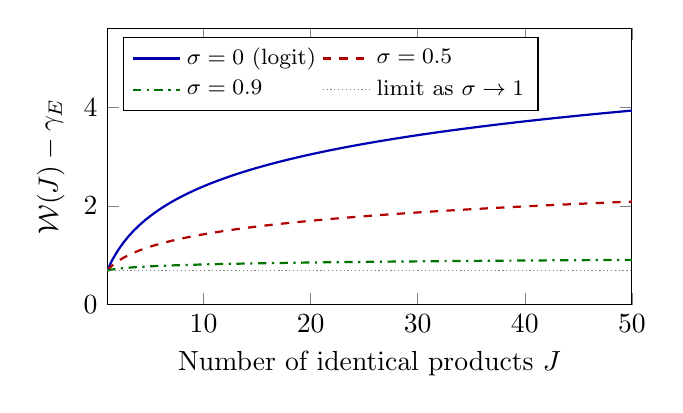
\begin{tikzpicture}
\begin{axis}[width=0.68\textwidth, height=0.42\textwidth,
  xlabel={Number of identical products $J$}, ylabel={$\mathcal{W}(J) - \gamma_E$},
  xmin=1, xmax=50, ymin=0, ymax=5.6, domain=1:50, samples=99,
  legend style={at={(0.03,0.97)}, anchor=north west, font=\footnotesize}, legend columns=2,
  legend cell align=left,
  every axis plot/.append style={thick}]
\addplot[blue!70!black] {ln(1 + x)};
\addlegendentry{$\sigma = 0$ (logit)}
\addplot[red!70!black, dashed] {ln(1 + x^0.5)};
\addlegendentry{$\sigma = 0.5$}
\addplot[green!45!black, dashdotted] {ln(1 + x^0.1)};
\addlegendentry{$\sigma = 0.9$}
\addplot[gray, thin, densely dotted] {ln(2)};
\addlegendentry{limit as $\sigma \rightarrow 1$}
\end{axis}
\end{tikzpicture}
\caption{Expected maximum utility with $J$ identical products in one nest, from \eqref{eq:07-clones} with mean
utility $\delta = 0$ and an outside good. Under the logit the value of variety grows like $\ln J$. The nested logit
slows the growth to $(1-\sigma)\ln J$, and only the limit $\sigma \to 1$ values fifty copies like one product.}
\label{fig:07-clones}
\end{figure}

\casehead{New goods and infinite virtual prices}
The \emph{virtual price} of a product is the price at which its demand falls to zero. Valuing a new good amounts to
integrating its demand curve from the virtual price down to the actual price \citep{Hausman1997}. In the logit the
share of $j$ is positive at every finite price, so the virtual price is infinite. The welfare integral still converges,
because the logit share decays exponentially in price. By the Roy identity of \cref{prop:07-logsum}, and because
$\Lambda$ approaches its value without $j$ as $p_j \to \infty$,
\begin{equation}\label{eq:07-newgood}
\int_{p_j}^{\infty}s_j(t)\,\dd t = \frac{1}{\alpha}\ln\frac{\Lambda^{\text{with } j}}{\Lambda^{\text{without } j}}
= -\frac{1}{\alpha}\ln\big(1 - s_j\big) ,
\end{equation}
where $s_j$ is the share of the new product after its introduction. This is \eqref{eq:07-removal-logit} with the sign
reversed. For small shares the value is close to $\frac{s_j}{\alpha}$. The logit markup of a single-product firm is
$\frac{1}{\alpha(1-s_j)}$, so its variable profit per consumer is $\frac{s_j}{\alpha(1-s_j)}$. The ratio of consumer
surplus to variable profit is $-\frac{(1-s_j)\ln(1-s_j)}{s_j}$, which lies below one and tends to one as $s_j \to 0$. In
the logit, a small new product therefore creates roughly as much consumer surplus as variable profit, whatever its
characteristics.

This mechanical link is the core of the critique of logit welfare analysis. \citet[p.~230]{Hausman1997} writes that the
IIA problem ``typically leads to a vast overestimate of the consumer's surplus from a new good.'' The reason, he adds,
is that ``the model does not incorporate sufficiently the similarities to existing goods.'' The CES demand system has the same feature: an
infinite virtual price and a gain from every new variety (\cref{ch:aids,ch:newgoods}). Nesting the new product with
close substitutes lowers its value through \eqref{eq:07-removal-nl}. Random coefficients let the data decide how
close the new product is to existing ones. \Citet{Trajtenberg1989} values CT scanners with a nested multinomial
logit, and \citet{Petrin2002} contrasts logit and random coefficients valuations of the minivan. \Cref{ch:newgoods}
covers both.

\subsection{Caveats}\label{sec:07-welfare-caveats}

\casehead{Income effects}
The log-sum formula relies on a constant marginal utility of income. Many applications instead use
$\alpha\ln(y_i - p_j)$, as \citet{BerryLevinsohnPakes1995} do, so that richer consumers are less price sensitive.
The marginal utility of income then varies across consumers and across the products they buy. Expected maximum
utility no longer converts into dollars by division by a constant, and the expected compensating variation must be
computed consumer by consumer. For each simulated consumer we draw the random coefficients and the shocks $e_{ij}$,
and we hold the draw fixed across the two choice sets. We then solve for the income change that makes her realized
maximum utility after the change equal to the one before it, and we average across consumers. Under the log form
each such compensation has a closed form (\cref{sec:10-petrin-cv}). The computation reuses the random coefficient
draws of the estimator of \cref{ch:blp} and adds draws of the shocks.

A tempting shortcut integrates out the shocks first. For each draw of the random coefficients, it solves for the
income change that restores expected maximum utility. The result is an ex ante compensation, paid before the shocks
are known, and it generally differs from the mean compensating variation. Take a consumer with income $y$ who has
only the outside good, with utility $\ln y + \epsilon_{i0}$, and add a free alternative with utility $\ln y +
\epsilon_{i1}$. The expected maximum of two independent standard type-I extreme value shocks exceeds that of one by
$\ln 2$, so restoring expected maximum utility requires $\ln(y - C) + \ln 2 = \ln y$, or $C = \frac{y}{2}$. The
realized compensation is $y\big[1 - e^{\epsilon_{i0} - \max(\epsilon_{i0}, \epsilon_{i1})}\big]$. Because
$\epsilon_{i1} - \epsilon_{i0}$ is logistic, the mean realized compensation is $(1 - \ln 2)y \approx 0.307y$. The two measures coincide when
utility is linear in income, so the log-sum formula needs no such distinction.

\casehead{What the shocks mean}
The welfare formulas treat the shocks $\epsilon_{ij}$ as tastes that consumers enjoy. \Cref{sec:07-logit-setup}
listed other readings, from unobserved characteristics to measurement error and mistakes. If the shocks are
mistakes, the log-sum counts them as real utility and overstates welfare. Under every reading, the model gives each
product its own dimension of taste and a group of consumers who prefer it. The result is positive shares, markups
of at least $\frac{1-\sigma}{\alpha}$, and positive value from every added product. This is the ``too many
characteristics'' problem. It biases estimated markups and the value of new goods upward, and it keeps products with zero
sales out of the direct inversion of observed shares. \Cref{sec:07-limits-epsilon} examines its consequences and the remedies proposed
in the literature.

\casehead{Scale and the outside good}
Welfare in dollars does not depend on the scale normalization of the shocks. Scaling all shocks by a constant scales
$\alpha$ and the mean utilities by the same constant, and the ratio in \eqref{eq:07-dcs} is unchanged. Welfare does
depend on the definition of the outside good and of market size, through \eqref{eq:07-dcs-s0}. A study that doubles the
assumed number of potential buyers changes $s_0$ in every market and changes every welfare number with it.

\section{Case study: Berry (1994) and the mean-utility method}\label{sec:07-berry}

The estimating equations of \cref{sec:07-inversion,sec:07-endogeneity,sec:07-supply,sec:07-nested} go back to
one article, \citet{Berry1994}. This section reads it in its own terms. We cite its equation numbers so that a
reader can follow the original, and we point back to the sections above for derivations already given. Page
numbers refer to the journal pagination.

\subsection{The question}\label{sec:07-berry-question}

Berry asks how to estimate demand and cost from a cross section of oligopoly markets with differentiated
products, when prices are correlated with demand factors that the econometrician does not observe. In
homogeneous-goods markets the demand error has long been read as unobserved demand factors, which the supply
relation shows to be correlated with price. Ignoring that correlation produces upward-sloping demand curves and
similar anomalies (p.~243). Berry argues that differentiated products raise the same problem whenever some
characteristics are unobserved, and that unobserved characteristics are common. Style is hard to quantify. Physically similar
products differ in perceived quality, durability, status or service. The relevant characteristics may outnumber
the observations.

Instrumental variables fix the problem for a homogeneous good. In a discrete-choice model, however, price and the
unobserved characteristic both enter the share equation nonlinearly, which blocks a direct application. The
alternatives of the time, reviewed in \cref{sec:07-inversion-problem}, were unattractive. A constant-elasticity
system (Berry's equation (1)) is linear, but $N$ goods bring $N^2$ elasticities, and restricting them a priori is
arbitrary. Discrete choice models without unobserved characteristics produce anomalies such as the
upward-sloping demand for CT scanners in \citet{Trajtenberg1989}. Berry derives demand from a utility model with
few parameters and finds a way to keep instrumental variables. The article is methodological. Its evidence is a
set of Monte Carlo experiments (\cref{sec:07-berry-mc}).

\subsection{The model}\label{sec:07-berry-model}

There are $R$ independent markets. Market $r$ has $N_r$ firms, each selling one product. Product $j$ has observed
characteristics $z_j = (x_j, w_j)$, where $x_j$ shifts demand and $w_j$ shifts marginal cost, an unobserved
demand characteristic $\xi_j$ and an unobserved cost shock $\omega_j$. Firms and consumers observe everything.
The econometrician observes prices, quantities and $z = (z_1, \dots, z_N)$.

\begin{assumption}[Exogenous characteristics]\label{asm:07-berry-exog}
In each market $(\xi_j, \omega_j)_{j=1}^N$ is mean independent of $z$, and markets are independent.
\end{assumption}

Berry himself calls this assumption ``unreasonable in many cases'' (p.~245). Utility is
\begin{equation}\label{eq:07-berry-utility}
u_{ij} = x_j\beta_i - \alpha p_j + \xi_j + \epsilon_{ij} = \delta_j + \mu_{ij} + \epsilon_{ij},
\qquad
\delta_j = x_j\beta - \alpha p_j + \xi_j ,
\end{equation}
with random coefficients $\beta_{ik} = \beta_k + \sigma_k\nu_{ik}$ and $\mu_{ij} = \sum_k x_{jk}\sigma_k\nu_{ik}$
(Berry's equations (2) to (5)). Berry writes $\tilde\beta_i$ and $\zeta_{ik}$ where we write $\beta_i$ and
$\nu_{ik}$, and he calls the composite deviation $v_{ij} = \mu_{ij} + \epsilon_{ij}$ by the name $\nu_{ij}$. The
mean utility $\delta_j$ collects everything common to all consumers.

\begin{remark}[What an i.i.d. shock restricts]\label{rem:07-berry-iid}
Let $\mu_{ij} = 0$, so that tastes vary only through a shock $\epsilon_{ij}$ that is i.i.d. across consumers and
products, with any continuous distribution. Then $s_j = s_j(\boldsymbol\delta)$, and since $p_k$ enters only
$\delta_k$, $\frac{\partial s_j}{\partial p_k} = -\alpha\frac{\partial s_j}{\partial\delta_k}$. Shares determine
$\boldsymbol\delta$ uniquely (\cref{prop:07-invertibility}), so products $j$ and $j'$ with equal shares have equal
mean utilities. Exchangeable shocks then give $\frac{\partial s_j}{\partial\delta_k} = \frac{\partial
s_{j'}}{\partial\delta_k}$, so $j$ and $j'$ have the same cross elasticity with respect to any third price
$p_k$. This holds whether $j$ and $j'$ are two subcompacts or a subcompact and a luxury car (p.~246). The
restriction comes from the i.i.d. additive error alone, so an i.i.d. probit shares it \citep{HausmanWise1978}.
Random coefficients remove it, because those who leave $j$ after a price rise have tastes $\beta_i$ that favor
products resembling $j$.
\end{remark}

Each consumer buys one unit of the best alternative. With $f(\cdot \mid x, \sigma)$ the density of
$\boldsymbol v_i$ and $A_j(\boldsymbol\delta) = \{\boldsymbol v_i : \delta_j + v_{ij} > \delta_k + v_{ik}\ \forall
k \ne j\}$, the share is $s_j = \int_{A_j(\boldsymbol\delta)} f(\boldsymbol v \mid x, \sigma)\,\dd\boldsymbol v$
(equation (6)), and quantity is $q_j = Ms_j$ (equation (7)). With finitely many consumers, observed shares
would carry sampling error of variance $\frac{s_j(1-s_j)}{M}$ (footnote 4), so Berry assumes a continuum. An
outside good, whose price does not respond to inside prices, ensures that a general price increase reduces
aggregate output (p.~247). Berry assumes $M$ is observed, as in BLP, where it is the number of households
(\cref{sec:07-market-size}).

Firm $j$ has costs $C_j(q_j, w_j, \omega_j, \gamma)$ and marginal cost $c_j$, so its profit is $p_jMs_j - C_j$
(equation (8)). At an interior pure-strategy Nash equilibrium in prices,
\begin{equation}\label{eq:07-berry-foc}
p_j = c_j + s_j\left|\frac{\partial s_j}{\partial p_j}\right|^{-1}
\end{equation}
(equation (9)).

\subsection{The inversion and the estimator}\label{sec:07-berry-inversion}

In $s_j = s_j(x, \boldsymbol p, \xi, \theta)$ (equation (10)) the error enters nonlinearly, so instrumental
variables do not apply directly. Berry transforms the shares so that $\xi$ appears linearly. With a known density
of consumer unobservables, $s_j = s_j(\boldsymbol\delta)$ (equation (11)), and the model fits observed shares
exactly at the true $\boldsymbol\delta$. The paper's Appendix shows that, with $\delta_0 = 0$, each interior share
vector is produced by exactly one $\boldsymbol\delta \in \R^N$ (\cref{prop:07-invertibility} reproduces the proof).
Inverting,
\begin{equation}\label{eq:07-berry-eq12}
\delta_j(s) = x_j\beta - \alpha p_j + \xi_j
\end{equation}
(equation (12)), the linear equation that \cref{sec:07-inversion-problem} motivates. When the density has
parameters $\sigma$, the
inverse depends on them, $\delta_j(s, \sigma) = x_j\beta - \alpha p_j + \xi_j$ (equation (21), which the paper
prints with $+\alpha p_j$ by a slip). With instruments satisfying $\E[\xi_j \mid z] = 0$ the estimator is
\begin{equation}\label{eq:07-berry-gmm}
\hat\theta = \argmin_{\theta}\ \xi(\theta)^\top Z W Z^\top \xi(\theta),
\qquad
\xi_j(\theta) = \delta_j(s, \sigma) - x_j\beta + \alpha p_j ,
\end{equation}
nonlinear in $\sigma$ \citep{Hansen1982} and two-stage least squares when $\sigma$ is known
(\cref{sec:07-estimator}). Each element of $\sigma$ requires an extra excluded instrument.

Berry's remarks on the structure of the data (pp.~249--250) appear in \cref{sec:07-inversion-logit}. With many
markets the $\xi_j$ may be correlated arbitrarily within a market, while a single market requires $\xi_j$
independent across firms (footnote 6). In both cases $\delta_j(s)$ plays the role that quantity plays in a
homogeneous-goods demand regression with cost instruments.

\subsection{Instruments as Berry states them}\label{sec:07-berry-instruments}

Berry names two families of demand instruments (p.~249), which \cref{sec:07-instruments} discusses at length.
The first is cost variables excluded from $x_j$, such as input prices that vary across firms. The second is the
characteristics of other firms, $x_k$ for $k \ne j$, which are excluded from $u_{ij}$ but correlated with $p_j$
through the markup in \eqref{eq:07-berry-foc}. \citet{BerryLevinsohnPakes1995} developed the second family into
the BLP instruments.

The logit makes the markup channel explicit. With single-product firms the markup is $\frac{1}{\alpha(1-s_j)}$
(\cref{prop:07-logit-markup}). At fixed prices, a rise in a rival's characteristic $x_{kl}$ changes $s_j$ by
$\frac{\partial s_j}{\partial\delta_k}\beta_l = -s_js_k\beta_l$, so the markup changes by
\begin{equation*}
\frac{\partial}{\partial x_{kl}}\left[\frac{1}{\alpha(1-s_j)}\right] = -\frac{s_js_k\beta_l}{\alpha(1-s_j)^2},
\end{equation*}
which is negative when $\beta_l > 0$. The rival characteristic moves $p_j$, while \cref{asm:07-berry-exog} makes it
uncorrelated with $\xi_j$. For the within-group share of the nested logit, Berry suggests ``the characteristics of
other firms in the group'' (p.~254). For the supply relation below he lists excluded demand characteristics,
rivals' characteristics, and market population as a shifter of output (p.~255).

\subsection{The worked examples}\label{sec:07-berry-examples}

\casehead{Logit}
With $\beta_i = \beta$ and type-I extreme value shocks, $s_j = \frac{e^{\delta_j}}{\sum_{k=0}^N e^{\delta_k}}$
(equation (13)), and with $\delta_0 = 0$,
\begin{equation}\label{eq:07-berry-eq14}
\ln s_j - \ln s_0 = x_j\beta - \alpha p_j + \xi_j
\end{equation}
(equation (14)), which is \eqref{eq:07-logit-inversion}. Berry calls the case unusual, since $\boldsymbol\delta$
must usually be found numerically, and notes that the logit ``produces unreasonable substitution patterns''
(p.~250).

\casehead{Vertical differentiation in Bresnahan's form}
In the vertical model of \citet{Bresnahan1987}, consumers agree on quality and disagree on its value:
$u_{ij} = \psi_j\nu_i - p_j$ with quality $\psi_j = x_j\beta + \xi_j$ (equations (15) and (16)). The taste
$\nu_i$ has distribution $F$ with density $f$ and mean one, which normalizes the units of quality and sets
$\alpha \equiv 1$. Order products so that $\psi_0 < \psi_1 < \dots < \psi_N$. Consumer $i$ prefers $j$ to $j-1$
when $\psi_j\nu_i - p_j > \psi_{j-1}\nu_i - p_{j-1}$, that is, when $\nu_i$ exceeds
\begin{equation*}
\Delta_j = \frac{p_j - p_{j-1}}{\psi_j - \psi_{j-1}}
\end{equation*}
(equation (17)). With $\Delta_0 = -\infty$, $\Delta_{N+1} = +\infty$ and increasing cutoffs, $i$ buys $j$ when
$\Delta_{j+1} > \nu_i > \Delta_j$, so
\begin{equation}\label{eq:07-berry-vert-share}
s_j = F(\Delta_{j+1}) - F(\Delta_j)
\end{equation}
(equation (18)). Solving for $\Delta_j$ from the top product down gives $\Delta_N = F^{-1}(1 - s_N)$ and
$\Delta_j = F^{-1}(F(\Delta_{j+1}) - s_j)$ (equation (19)). With $\psi_0 = p_0 = 0$, the cutoff definition then
yields $\psi_j = \psi_{j-1} + \frac{p_j - p_{j-1}}{\Delta_j}$ (equation (20)), and $\delta_j = \psi_j - p_j$. If
$\E[\xi_j \mid x] = 0$, least squares of $\psi_j$ on $x_j$ estimates $\beta$, with no price instrument, because
price is not a regressor. Berry calls the two examples opposite extremes (p.~251). The logit has one taste shock
per product and makes all products substitutes. The vertical model has one taste and makes only quality
neighbors substitutes. \Cref{ch:discrete} derives the same recursion for the form $u_{ij} = \delta_j - \nu_ip_j$.

\casehead{Nested logit through the group share}
Following \citet{Cardell1997}, products fall into groups $g = 0, 1, \dots, G$ with the outside good alone in
group $0$, and for $j \in g$
\begin{equation*}
u_{ij} = \delta_j + \zeta_{ig} + (1 - \sigma)\epsilon_{ij}
\end{equation*}
(equation (22)), with $\zeta_{ig}$ distributed as in \cref{lem:07-cardell}. Writing $\zeta_{ig}$ as $\sum_h
d_{jh}\zeta_{ih}$ with group dummies $d_{jh}$ shows a random-coefficients model with random coefficients on group
dummies only, so correlation depends on groupings fixed before estimation (p.~253). The shares (equations (23) to
(25)) are those of \cref{prop:07-nl-shares}, with $D_g = \sum_{k \in g} e^{\frac{\delta_k}{1-\sigma}}$, group share
$s_g = \frac{D_g^{1-\sigma}}{\sum_h D_h^{1-\sigma}}$ and $D_0 = 1$, so that $s_0 = \frac{1}{\sum_h
D_h^{1-\sigma}}$. Taking logs of $s_j$ and $s_0$,
\begin{equation}\label{eq:07-berry-eq26}
\ln s_j - \ln s_0 = \frac{\delta_j}{1-\sigma} - \sigma\ln D_g
\end{equation}
(equation (26)). Berry removes the unobserved $D_g$ with the group share. Since $\frac{s_g}{s_0} = D_g^{1-\sigma}$,
we have $\ln D_g = \frac{\ln s_g - \ln s_0}{1-\sigma}$. Substituting into \eqref{eq:07-berry-eq26}, multiplying by
$1-\sigma$, and solving for $\delta_j$,
\begin{align*}
\delta_j &= (1-\sigma)(\ln s_j - \ln s_0) + \sigma(\ln s_g - \ln s_0) \\
&= \ln s_j - \sigma(\ln s_j - \ln s_g) - \ln s_0 = \ln s_j - \sigma\ln s_{j\mid g} - \ln s_0
\end{align*}
(equation (27)), because $s_{j\mid g} = \frac{s_j}{s_g}$. Substituting $\delta_j = x_j\beta - \alpha p_j + \xi_j$
gives $\ln s_j - \ln s_0 = x_j\beta - \alpha p_j + \sigma\ln s_{j\mid g} + \xi_j$ (equation (28)), which is
\eqref{eq:07-nl-regression}. \Cref{sec:07-nl-estimation} eliminates $D_g$ through the within-group share
instead, and both routes reach the same equation.

\casehead{Random coefficients}
In the full model the inversion is numerical, and the share integral needs simulation \citep{Pakes1986}, as
developed by \citet{BerryLevinsohnPakes1995}. Berry sees a trade-off (p.~254). The nested logit suits costly
computation or predetermined classes of products, and random coefficients suit richer substitution patterns.
\Cref{tab:07-berry-examples} summarizes the examples, including the pricing equations derived next.

\begin{table}[htbp]
\centering
\caption{The examples of \citet{Berry1994}: inversion, pricing equation, and instruments}
\label{tab:07-berry-examples}
\small
\renewcommand{\arraystretch}{1.5}
\begin{tabularx}{\linewidth}{>{\raggedright\arraybackslash}p{0.16\linewidth}
  >{\raggedright\arraybackslash}p{0.25\linewidth}
  >{\raggedright\arraybackslash}p{0.26\linewidth}
  >{\raggedright\arraybackslash}X}
\toprule
Model & Mean utility $\delta_j(s)$ & Single-product markup $p_j - c_j$ & Extra parameters and instruments \\
\midrule
Logit, eqs.\ (13), (14), (31) & $\ln s_j - \ln s_0$ & $\frac{1}{\alpha(1-s_j)}$ &
  None beyond one excluded instrument for $p_j$ (cost shifters, rivals' $x_k$) \\
Nested logit, eqs.\ (22) to (28), (33) & $\ln s_j - \sigma\ln s_{j\mid g} - \ln s_0$ &
  $\frac{1-\sigma}{\alpha\,[1 - \sigma s_{j\mid g} - (1-\sigma)s_j]}$ &
  $\sigma$, with characteristics of other firms in the group as instruments for $\ln s_{j\mid g}$ \\
Vertical, eqs.\ (15) to (20), (32) & $\psi_j - p_j$, from the recursion for $\Delta_j$ and $\psi_j$ &
  $s_j\left[\frac{f(\Delta_{j+1})}{\psi_{j+1}-\psi_j} + \frac{f(\Delta_j)}{\psi_j-\psi_{j-1}}\right]^{-1}$ &
  None if $F$ is known ($\alpha \equiv 1$), else the parameters of $F$ \\
Random coefficients, eqs.\ (2) to (6) & Numerical inversion (\cref{ch:blp}) &
  $\frac{1}{\alpha}\,s_j\big(\frac{\partial s_j}{\partial\delta_j}\big)^{-1}$, numerical &
  $(\sigma_k)$, with at least one extra instrument per $\sigma_k$ \\
\bottomrule
\end{tabularx}
\par\medskip
\parbox{\linewidth}{\footnotesize Notes: Equation numbers are those of \citet{Berry1994}. All markups assume
single-product Nash pricing. In the vertical model the term in $f(\Delta_{N+1})$ is zero for the top product.}
\end{table}

\subsection{The pricing equation and joint estimation}\label{sec:07-berry-supply}

Section 6 of the paper adds the first-order conditions. Price enters only through $\delta_j$, so $\frac{\partial
s_j}{\partial p_j} = -\alpha\frac{\partial s_j}{\partial\delta_j}$, and given the density both $\delta_j$ and
$\frac{\partial s_j}{\partial\delta_j}$ are known functions of the data. With marginal cost $c_j = \bar c(q_j, w_j,
\gamma) + \omega_j$, \eqref{eq:07-berry-foc} becomes
\begin{equation}\label{eq:07-berry-eq29}
p_j = \bar c(q_j, w_j, \gamma) + \frac{1}{\alpha}\,s_j\left(\frac{\partial s_j}{\partial\delta_j}\right)^{-1} +
\omega_j
\end{equation}
(equation (29)). The regressors $q_j$, $s_j$ and $\frac{\partial s_j}{\partial\delta_j}$ are correlated with
$\omega_j$ and need the instruments listed above. Demand (equation (21)) and supply (equation (29)) share $\alpha$
and $\sigma$, and joint estimation imposes these cross-equation restrictions (p.~255). The moments are $\E[z^d_j
\xi_j(\theta)] = 0$ and $\E[z^s_j\omega_j(\theta)] = 0$, with $\omega_j(\theta)$ the residual of
\eqref{eq:07-berry-eq29} at $\boldsymbol\delta(s, \sigma)$ (\cref{sec:07-cost-recovery}).

With $c_j = w_j\gamma + \omega_j$ (equation (30)), the analytic examples give the markups of
\cref{tab:07-berry-examples}. The logit gives $p_j = w_j\gamma + \frac{1}{\alpha}\frac{1}{1-s_j} + \omega_j$
(equation (31)), so the supply side estimates $\frac{1}{\alpha}$ directly. In the vertical model,
$\frac{\partial\Delta_{j+1}}{\partial p_j} = -\frac{1}{\psi_{j+1}-\psi_j}$ and $\frac{\partial\Delta_j}{\partial
p_j} = \frac{1}{\psi_j - \psi_{j-1}}$, so differentiating \eqref{eq:07-berry-vert-share} gives the markup in the
table. Price minus markup, $y_j = w_j\gamma + \omega_j$, is then data, and $\gamma$ follows from least squares
(equation (32)). The nested logit gives
\begin{equation}\label{eq:07-berry-eq33}
p_j = w_j\gamma + \frac{1-\sigma}{\alpha\,[1 - \sigma s_{j\mid g} - (1-\sigma)s_j]} + \omega_j
\end{equation}
(equation (33)), the single-product case of \cref{prop:07-nl-markup}. At $\sigma = 0$ only $s_j$ affects the
markup, and as $\sigma \to 1$ only $s_{j\mid g}$ does. So the joint behavior of prices, product shares and group
shares helps identify $\sigma$ (p.~256).

\subsection{Why the obvious alternatives fail}\label{sec:07-berry-alternatives}

Section 7 of the paper rejects three alternatives, which \cref{sec:07-inversion-problem} develops in detail.
Estimating each $\xi_j$ as a fixed effect fails by the logic of grouped data. Integrating $\xi$ out of the share
function at fixed prices contradicts the pricing equation \eqref{eq:07-berry-foc}, because prices respond to $\xi$.
The reduced form of \citet{Bresnahan1987} and \citet{Berry1990} (equations (34) and (35)) tolerates measurement error
in prices and quantities, which is how Bresnahan models the error. It needs costly integrals over implicitly defined
functions, however, and a unique equilibrium for almost all values of the unobservables. \citet{CaplinNalebuff1991}
prove uniqueness for the logit and the vertical model, exactly the cases where the inversion is easy. The
mean-utility method ``does not rely on the existence of a unique equilibrium'' (p.~243).

\subsection{Monte Carlo evidence}\label{sec:07-berry-mc}

\Cref{sec:07-montecarlo} states Berry's design in \eqref{eq:07-mc-design} and replicates it. Each simulated
sample has 500 duopoly markets with Bertrand-Nash prices (p.~258). Each design has 100 samples, estimated by least
squares and by instrumental variables with $w_j$ and the rival's $x_k$ as instruments. The non-price part of mean
utility has variance $\beta_x^2 + \sigma_d^2$. With $\sigma_d = 1$ the observed $x_j$ accounts for $\frac{4}{5}$ of
it, and with $\sigma_d = 3$ the unobserved term accounts for $\frac{9}{13}$, almost 70 percent.\footnote{Later on
the same page Berry says the observed characteristic accounts for ``only 25\%'' in this design. The stated
parameters imply $\frac{4}{13}$, about 31 percent.}

Berry's Table 1 sits next to our replication in \cref{tab:07-mc-logit}. With $\sigma_d = 1$, least squares gives
$\hat\alpha = 0.726$ (0.029) and instrumental variables 0.995 (0.039), against a true value of 1. With
$\sigma_d = 3$ the figures are 0.181 (0.076) and 0.979 (0.128). The coefficients on $x_j$ and the constant show
the same pattern (\cref{tab:07-mc-logit}). Prices rise with $\xi_j$ through the markup and through cost, so by \cref{prop:07-ols-bias} least squares understates $\alpha$,
and more so when $\sigma_d$ is large. In many samples the least-squares estimate implies pricing on the inelastic
part of demand, and with $\sigma_d = 3$ it sometimes implies upward-sloping demand. \Cref{tab:07-blp-logit,%
tab:07-nevo-logit} show the same pattern in field data.

\subsection{Interpretation, limitations, and contribution}\label{sec:07-berry-assessment}

Berry's conclusion states the idea: mean utilities ``can then be treated in much the same fashion as observed
output quantities in the homogeneous goods model'' (p.~260). The demand side needs no distribution for $\xi$, no
model of price setting and no unique equilibrium. A supply side can be added when the researcher accepts Nash
pricing.

Berry lists the main limitations himself (pp.~258--260). Demand is static and single-unit, and the taste
distribution is known up to parameters. The inversion ``may be quite sensitive'' to measurement error in shares.
Characteristics are assumed exogenous, and a solution ``awaits further progress on dynamic models of firm
behavior.'' Berry also flags two data problems that later work developed. His Section 9 lists the estimation of the
market size $M$ as open and points to \citet{Berry1990} and \citet{Greenstein1992} (p.~258). His footnote 4 notes
that with $M$ distinct consumers the observed shares carry sampling error with variance $\frac{s_j(1 - s_j)}{M}$,
which he assumes away by treating consumers as a continuum (p.~247).
\citet*{BerryLintonPakes2004} develop limit theory as the number of products grows, allowing for sampling error in
the shares and simulation error in the predicted shares. The estimator is asymptotically normal if the consumer sample
and the number of simulation draws grow fast enough relative to the number of products. \Cref{sec:07-market-size}
shows how results depend on the assumed market size.
A third problem, zero shares, breaks the inversion \citep{GandhiLuShi2023}. The analytic examples also inherit logit
substitution patterns and assume single-product firms (\cref{sec:07-bertrand-multi} treats multi-product pricing).

Berry states what any extension must supply (p.~259). A richer utility model needs its own invertibility result,
showing that given the parameters each vector of observed shares is explained by one vector of demand
unobservables. A richer pricing model needs an analogue of equation (29), showing that data and parameters together
determine the cost unobservable.

The article made instrumental-variables estimation the default for discrete-choice demand on aggregate data.
Berry notes that his model implies a hedonic equilibrium pricing function of product characteristics, which links it
to the hedonic literature (p.~244, n.~1). Its focus on price-setting firms and unobserved characteristics differs
from the typical hedonic study. He reports two early applications (p.~260). The working-paper version of
\citet{BerryLevinsohnPakes1995} found that allowing for unobserved characteristics correlated with prices improves
the estimated own-price elasticities. \citet{Greenstein1992} estimated a vertical model of the computer industry with unobserved characteristics.
\citet{BerryLevinsohnPakes1995} added random coefficients, simulation, a contraction for the inversion and
approximate optimal instruments (\cref{ch:blp}). Invertibility was later shown under weaker conditions
\citep{BerryGandhiHaile2013}, and nonparametric identification was studied by \citet{BerryHaile2014}. The method
underlies \citet{Einav2007} below, \citet{Nevo2001} in \cref{ch:blp}, \citet{BerryCarnallSpiller2006} in
\cref{ch:airlines} and merger simulation in \cref{ch:mergers}, and standard software implements it
\citep{ConlonGortmaker2020}.

\section{Case study: Einav (2007), seasonality in motion pictures}\label{sec:07-einav}

\citet{Einav2007} uses a one-nest nested logit for a purpose far from price elasticities. Ticket prices are nearly
uniform, so the paper estimates no price coefficient. The model separates two sources of seasonal sales: demand
that varies over the year, and the number and quality of movies on offer.

\subsection{Question, setting, and data}\label{sec:07-einav-setting}

Moviegoing sometimes more than doubles within two weeks, and the first week brings almost 40 percent of an average
movie's box office (p.~127). With virtually no price competition, the release date is a main short-run strategic
variable, and timing decisions create a seasonal pattern in releases. Observed seasonality thus mixes underlying
demand with the number and quality of available movies. The split matters for strategy. If demand drives
seasonality, distributors should release when demand is high. If quality drives it, they should release in low
seasons, when competition is soft. Einav calls a market response that reinforces demand swings, for example more
or better movies in high seasons, an \emph{amplification effect}. A response that offsets them, such as higher
prices in high seasons, is a \emph{dampening effect} (p.~128).

Distributors set release dates, negotiate with exhibitors and run national advertising (pp.~129--130). A wide
release opens in typically several thousand theaters at once. Exhibitors pay the greater of 90 percent of revenue
net of house expenses or a share of gross revenue that starts near 70 percent and then declines. Distributors
collect about half of box office. Domestic box office is now about 15 percent of a movie's revenue,
but it drives ancillary revenue, so Einav takes it as the distributor's objective.

The data cover all movies released in the United States from 1985 to 1999 (ACNielsen EDI). They give weekly
revenue and screens for the first 10 weeks, which bring more than 90 percent of revenue (pp.~131--132). Weekly shares are
revenue divided by the ticket price and the U.S. population, both interpolated from annual figures. Children and
senior citizens buy discounted tickets, so this calculation understates the shares of movies aimed at them. The
fraction of discounted tickets varies mainly across movies and little within a movie, so the movie fixed effects
address this concern (footnote 11). Of 3,523
titles, Einav keeps those that reach a wide release of at least 600 screens in some week. He drops 97 titles
with a long platform release that did not reach a wide release within 10 weeks of their official release date.
He also leaves out the first nine weeks of 1985 (footnote 13). The final sample has 1,956 titles, 16,103 weekly
observations and 94 percent of revenue. Mean total revenue is \$34.8 million and the median \$20.0 million. The
share of the population that sees a movie in its first ten weeks averages 2.78 percent, with a median of 1.71
percent. Production cost, reported for 1,604 titles, averages \$29.7 million in December 1999 dollars (Table 2).
Table 1 reports industry trends. In December 1999 dollars the average ticket price was \$5.54 in 1985 and \$5.00 in
1999. Over the same years wide releases rose from 103 to 143 a year, and the industry share, annual admissions over
the U.S. population, grew from 2.69 to 5.03 (pp.~131--132). Holidays
shift from year to year, so 56 calendar-week dummies keep each holiday in a fixed week, for example Labor Day in
week 38 and Thanksgiving in week 51.

\subsection{The model}\label{sec:07-einav-model}

Consumer $i$'s utility from movie $j$ in week $t$ and from not going to the movies are
\begin{equation}\label{eq:07-einav-u}
u_{ijt} = \phi_j - \lambda(t - r_j) + \xi_{jt} + \zeta_{it} + (1-\sigma)\epsilon_{ijt},
\qquad
u_{i0t} = -\tau_t + \zeta'_{it} + (1-\sigma)\epsilon_{i0t}
\end{equation}
(Einav's equations (1) and (2)). The quality $\phi_j$ is written $\theta_j$ in the paper, and we rename it because
$\theta$ is the conduct parameter in this book. The release week is $r_j$, $\lambda$ is a common weekly decay,
and $\xi_{jt}$ is a movie-week deviation from it. The week effect $\tau_t$ enters the outside good, so underlying
seasonality is the time-varying value of not going to the movies, which Einav reads as the opportunity cost of
time. The shocks $\epsilon$ are type-I extreme value and $\zeta_{it}$, $\zeta'_{it}$ have Cardell's distribution, so
movies form one nest and the outside good another.

Adding $\tau_t$ to every alternative leaves choices unchanged, sets the outside good's mean utility to zero, and
gives movie $j$ the mean utility $\delta_{jt} = \phi_j - \lambda(t - r_j) + \tau_t + \xi_{jt}$.
\Cref{prop:07-nl-shares} with one inside nest, the set $\mathcal{J}_t$ of movies showing in week $t$, gives
\begin{equation*}
s_{jt} = \frac{e^{\frac{\delta_{jt}}{1-\sigma}}}{D_t}\cdot\frac{D_t^{1-\sigma}}{1 + D_t^{1-\sigma}}
= \frac{e^{\frac{\delta_{jt}}{1-\sigma}}}{D_t^{\sigma} + D_t},
\qquad
D_t = \sum_{k \in \mathcal{J}_t} e^{\frac{\delta_{kt}}{1-\sigma}}
\end{equation*}
(equations (3) and (4)). The inversion of \cref{prop:07-nl-inversion}, with within-industry share
$\frac{s_{jt}}{1-s_{0t}}$, then gives the estimating equation
\begin{equation}\label{eq:07-einav-est}
\ln s_{jt} - \ln s_{0t} = \phi_j + \tau_t - \lambda(t - r_j) + \sigma\ln\frac{s_{jt}}{1 - s_{0t}} + \xi_{jt}
\end{equation}
(equation (5)). Movie effects capture cast, plot and prerelease advertising, which Einav treats as fixed effects
because observables explain little of quality. The dependent variable is close to log revenue, so linear decay is
proportional decay, reflecting saturation and a preference for seeing movies early. As $\sigma \to 0$ the model is
a simple logit. As $\sigma \to 1$ movies stop drawing from the outside good, so a new movie only steals from other
movies. Lower $\sigma$ attributes more seasonality to the number and quality of movies.

The paper writes the decay as $-\lambda(t - r_j)$ but reports the estimated coefficient on $t - r_j$, which is
$-\lambda$. Its benchmark estimate of $-0.220$ means $\lambda = 0.220$, the value its later calculations use.
\Cref{tab:07-einav-benchmark} prints coefficients as the paper does.

\subsection{Identification and estimation}\label{sec:07-einav-identification}

Two assumptions do the work (p.~135). The decay of mean utility is orthogonal to the release date, which identifies
movie qualities. Variation across years in the number of movies released in a given calendar week is exogenous,
which identifies market expansion.

There is one national market, so the same movie cannot be observed released on different dates. Weekly revenues
give several observations per movie instead. A movie released in a high-demand week keeps playing in later weeks,
under different seasonal demand and against different rivals. Comparing movies observed in the same weeks
identifies relative qualities, and 15 years supply many choice sets per calendar week. Einav's example shows the
logic.

\begin{example}[Einav's two-season example]\label{ex:07-einav-toy}
A year has two seasons of market sizes $1$ and $M > 1$, and two movies are released per year, one per season, of
qualities $1$ and $\phi_H > 1$. A movie of quality $\phi$ in a season of size $m$ sells $m\phi$, and the better
movie is always released in season 2. If each movie plays for one season, sales are $1$ and $M\phi_H$, and only
the product $M\phi_H$ is identified. Suppose instead that each movie plays two seasons, with quality multiplied by a
common factor $d < 1$ in the second. With $R_{q,m}$ the sales of the quality-$q$ movie in the season of size $m$,
\begin{equation*}
R_{1,1} = 1, \qquad R_{1,M} = Md, \qquad R_{H,M} = M\phi_H, \qquad R_{H,1} = d\phi_H .
\end{equation*}
The last three equations have three unknowns. Since $\frac{R_{1,M}R_{H,M}}{R_{H,1}} = M^2$,
\begin{equation*}
M = \sqrt{\frac{R_{1,M}R_{H,M}}{R_{H,1}}}, \qquad d = \frac{R_{1,M}}{M}, \qquad \phi_H =
\frac{R_{H,M}}{M}.
\end{equation*}
With our illustrative values $M = 2$, $\phi_H = 1.5$ and $d = 0.5$, the data are $R_{1,M} = 1$, $R_{H,M} =
3$ and $R_{H,1} = 0.75$, and the formulas return $M = \sqrt{\frac{3}{0.75}} = 2$, $d = 0.5$ and $\phi_H =
1.5$. If decay differed by release season, a fourth unknown would break identification.
\end{example}

With more movies and seasons, decay may differ across movies, provided it does not vary with the release date
once observables are controlled for. The assumption concerns the decay of utility. Revenue decay does depend on
the release date, through seasonal demand. The main
threat is that studios know decay and release fast-decay movies late in the summer. Einav replies that the
industry thinks in terms of expected total revenue and that decay is predictable ex post more than ex ante. The
assumption is also more plausible for movies released close together (p.~136). \Cref{sec:07-einav-robust} tests it.

Market expansion is identified from the long panel. If more or better movies open on Memorial Day 1999 than in
1998, similar total revenues imply weak expansion ($\sigma$ near one) and higher revenues imply strong expansion
(low $\sigma$). The within-industry share rises with $\xi_{jt}$, so it needs an instrument. The benchmark uses the
number of movies showing in the week, $n_t$, since more movies lower each movie's within-industry share. Week
dummies absorb any tendency to release more movies in high-demand weeks, so the identifying variation is across
years within a calendar week. Movie effects absorb the quality of a strong movie that deters rivals. The remaining
requirement is that $n_t$ is uncorrelated with the decay shocks $\xi_{jt}$. Variation comes from production
uncertainty: projects are committed a year or two ahead, completion and quality are uncertain, and studios avoid
holding finished movies (pp.~136--137). The estimator is two-stage least squares of \eqref{eq:07-einav-est} with
1,956 movie effects, 56 week dummies and the decay term, and $n_t$ as the excluded instrument.

\subsection{Results}\label{sec:07-einav-results}

\Cref{tab:07-einav-benchmark} and \cref{fig:07-einav-seasonality} report the benchmark. Controlling for movie
quality dampens estimated seasonality. The standard deviation of the week coefficients is 0.238 with movie fixed
effects and 0.356 without (p.~138). Endogenous quality thus amplifies seasonality by about 50 percent, since
$\frac{0.356}{0.238} \approx 1.50$. In the paper's summary, about a third of seasonal variation in sales comes
from the number and quality of movies (pp.~129 and 143).

\begin{table}[htbp]
\centering
\caption{Benchmark estimates and subperiod decay in \citet{Einav2007}}
\label{tab:07-einav-benchmark}
\small
\begin{tabular}{lccc}
\toprule
\multicolumn{4}{l}{\textit{Panel A. Benchmark model (inset table of Figure 3)}} \\
 & With movie FE & Without movie FE & \\
\midrule
Weeks since release $t - r_j$ (coefficient $= -\lambda$) & $-0.220$ & $-0.163$ & \\
 & (0.0014) & (0.005) & \\
Nesting parameter $\sigma$ & 0.524 & 0.577 & \\
 & (0.030) & (0.011) & \\
Number of observations & 16,103 & 16,103 & \\
Number of titles & 1,956 & 1,956 & \\
$R^2$ & 0.876 & 0.893 & \\
\midrule
\multicolumn{4}{l}{\textit{Panel B. Benchmark model by subperiod, $\sigma$ fixed at 0.524 (inset table of
Figure 5)}} \\
 & 1985--1989 & 1990--1994 & 1995--1999 \\
\midrule
Weeks since release $t - r_j$ (coefficient $= -\lambda$) & $-0.174$ & $-0.206$ & $-0.253$ \\
 & (0.0016) & (0.0014) & (0.0015) \\
Number of observations & 4,035 & 5,521 & 6,547 \\
Number of titles & 572 & 666 & 754 \\
$R^2$ & 0.402 & 0.430 & 0.499 \\
\bottomrule
\end{tabular}
\par\medskip
\parbox{\linewidth}{\footnotesize Notes: Two-stage least squares of \eqref{eq:07-einav-est}. Standard errors in
parentheses. All specifications include 56 calendar-week dummies. The instrument for the log within-industry share
is the number of movies showing in the week. In Panel B the unconstrained estimates of $\sigma$ are 0.40, 0.74 and
0.70 (Einav's footnote 18). Source: \citet{Einav2007}, insets of Figures 3 and 5.}
\end{table}

\begin{figure}[htbp]
\centering
\begin{subfigure}[b]{0.49\textwidth}
\centering
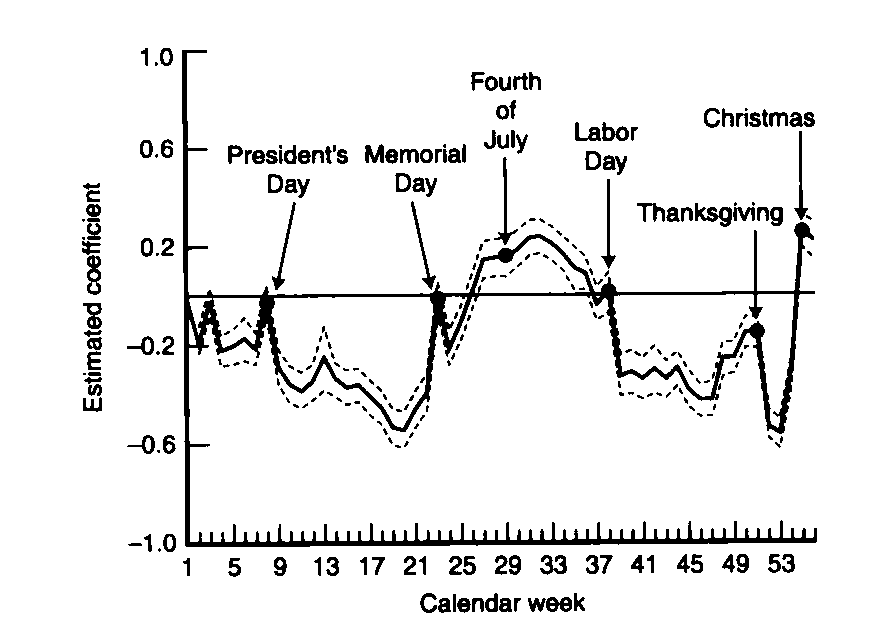
\includegraphics[width=\linewidth]{figures/ch07/einav_fig3_top.png}
\caption{With movie fixed effects}
\end{subfigure}\hfill
\begin{subfigure}[b]{0.49\textwidth}
\centering
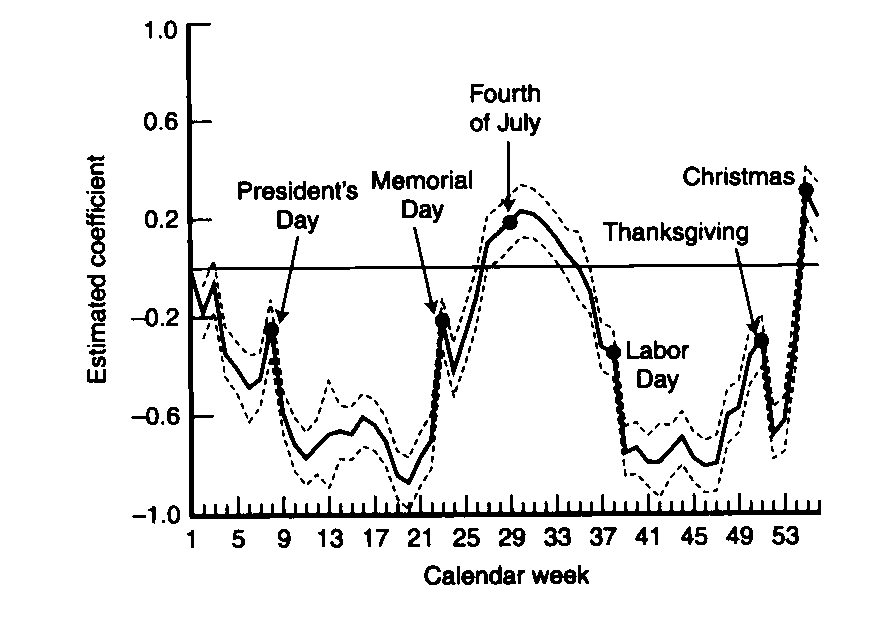
\includegraphics[width=\linewidth]{figures/ch07/einav_fig3_bottom.png}
\caption{Without movie fixed effects}
\end{subfigure}
\caption{Estimated week effects $\hat\tau_t$ by calendar week in the benchmark model of \citet{Einav2007}.
Panel (a) is the top panel and panel (b) the bottom panel of the original figure. Dashed lines mark two standard
errors. Source: \citet{Einav2007}, Figure 3.}
\label{fig:07-einav-seasonality}
\end{figure}

Underlying demand resembles revenue, high in summer and the holidays and low in spring and fall, but the
differences are informative (p.~138). Memorial Day, the Fourth of July and Thanksgiving, the big release weekends,
have high underlying demand, though less so relative to adjacent weeks than revenues suggest. Labor Day, when few
movies open, has much higher underlying demand than its revenue implies. Underlying demand is flat over the summer
and drops sharply after Labor Day, whereas revenues peak in early July and decline gradually, because the biggest
movies open early in the summer.

With $\lambda = 0.220$ and $\hat\sigma = 0.524$, Einav reports weekly revenue decay of 37 percent. For a movie too
small to move $D_t$, $\ln s_{jt}$ equals $\frac{\delta_{jt}}{1-\sigma}$ plus terms in $D_t$, so one more week
changes log share by $-\frac{0.220}{0.476} = -0.462$, and $1 - e^{-0.462} = 0.37$. Ten decay dummies give an almost
linear pattern. A linear time trend is not identified (footnote 19). If mean utility included $b\,t$, writing
$b\,t = b\,r_j + b(t - r_j)$ shows that it loads onto the movie effects, $\phi_j + b\,r_j$, and
onto the decay, $\lambda - b$. The movie effects, which show no trend, measure quality relative to an outside
good that may itself be changing.

\Cref{tab:07-einav-fe} projects the estimated movie effects on observables. Production cost, advertising and
Oscar recognition raise estimated quality, and restrictive ratings lower it. The adjusted $R^2$ is at most 0.387,
which Einav reads as the justification for fixed effects.

\begin{table}[htbp]
\centering
\caption{Projection of the estimated movie fixed effects on observables \citep[Table 3]{Einav2007}}
\label{tab:07-einav-fe}
\small
\begin{tabular}{lccc}
\toprule
Dependent variable: estimated movie effect $\hat\phi_j$ & (1) & (2) & (3) \\
\midrule
Log production cost & 0.215$^{**}$ (0.021) & 0.389$^{**}$ (0.021) & 0.384$^{**}$ (0.020) \\
Log advertising expenditure & 0.367$^{**}$ (0.019) & & \\
MPAA rating PG-13 & $-0.125^{**}$ (0.038) & $-0.135^{**}$ (0.043) & \\
MPAA rating R & $-0.154^{**}$ (0.039) & $-0.144^{**}$ (0.044) & \\
MPAA rating above R & $-0.442$ \phantom{$^{**}$}(0.365) & $-0.716^{*}$ \phantom{$^{*}$}(0.413) & \\
Genre comedy & $-0.052$ \phantom{$^{**}$}(0.035) & 0.029 \phantom{$^{**}$}(0.039) & \\
Genre drama & $-0.097^{**}$ (0.037) & $-0.021$ \phantom{$^{**}$}(0.040) & \\
Genre children & $-0.070$ \phantom{$^{**}$}(0.054) & $-0.037$ \phantom{$^{**}$}(0.060) & \\
Best picture nominee & 0.433$^{**}$ (0.081) & & \\
Best picture award & 0.467$^{**}$ (0.139) & & \\
Year fixed effects & yes & yes & no \\
$N$ & 1,542 & 1,603 & 1,603 \\
Adjusted $R^2$ & 0.387 & 0.208 & 0.193 \\
\bottomrule
\end{tabular}
\par\medskip
\parbox{\linewidth}{\footnotesize Notes: Standard errors in parentheses. $^{*}$ significant at the 10 percent
level, $^{**}$ at the 1 percent level. Omitted categories are rating PG and genre action. Blank cells are
variables not included. Samples are smaller than 1,956 because production cost and advertising are missing for
some movies. Source: \citet{Einav2007}, Table 3.}
\end{table}

\subsection{Robustness}\label{sec:07-einav-robust}

Predicted shares reproduce the observed seasonal pattern well, but the model underpredicts revenue in early summer
and the holidays and overpredicts it elsewhere (Figure 4, p.~139). Movies released in strong seasons decay more
slowly. Interacting decay with movie size, instrumented by production cost times decay, shows that better movies
decay more slowly and improves fit, but underlying seasonality barely moves. Letting decay vary by release season
gives $-0.194$ for holiday releases, $-0.206$, $-0.216$ and $-0.214$ for winter, spring and early summer, and
$-0.249$ and $-0.244$ for late summer and fall (pp.~139--140). Equality of the first four is not rejected, and
equality of the last two with the others is rejected. The summer week effects are unchanged.

Results are almost identical after dropping the first three weeks of each run, for movies with a full 10-week run
and for Friday releases (p.~140). Panel B of \cref{tab:07-einav-benchmark} shows faster decay in later
subperiods, consistent with wider openings, while underlying seasonality is stable. Alternative instruments, the
budget of competing movies, the number in the same genre, or the number released within a three-week or five-week
window, give similar results. The window counts address one source of endogeneity. Fewer movies may be shown in a week
when a strong movie is released. If distributors can move a release date by only a few weeks, counts over a window
around the week account for this response (footnote 20). Instruments
interacted with a measure of the movie's ex-ante size, such as production cost, are weaker. They give low estimates
of $\sigma$ and somewhat different results, but adding them to the main instruments leaves the reported results in
place (footnote 21). The nested logit ties expansion from more movies to expansion from better movies
through one parameter. \citet{AckerbergRysman2005} suggest adding the log number of products as a regressor, which
here is the instrument. Including it through functional form or with other instruments changes little
(pp.~140--141).

\subsection{Implications for release dates}\label{sec:07-einav-timing}

Set $\xi_{jt} = 0$ and write $Q_{kt} = \exp\big(\frac{\phi_k - \lambda(t-r_k)}{1-\sigma}\big)$ for the
decay-adjusted quality index and $C_t = \sum_{k \in \mathcal{J}_t} Q_{kt}$ for the \emph{competition effect}. Since
$D_t = \exp\big(\frac{\tau_t}{1-\sigma}\big)C_t$, dividing numerator and denominator of $s_{jt}$ by
$\exp\big(\frac{\tau_t}{1-\sigma}\big)$ gives
\begin{equation}\label{eq:07-einav-eq6}
s_{jt} = \frac{Q_{jt}}{C_t^{\sigma}}\,\Big[e^{-\tau_t} + C_t^{1-\sigma}\Big]^{-1}
\end{equation}
(Einav's equation (6)). The market-size term $e^{-\tau_t}$ is small when underlying demand is high. Competition
matters more as $\sigma$ rises, because movies then steal more from each other. With fixed prices and nearly zero
marginal cost, a price-taking distributor picks $r_j$ to maximize $\sum_{t=r_j}^{r_j+H}s_{jt}$ for a horizon $H$,
taking rivals' dates as given (pp.~141--142). Competition peaks at the start of the summer and at Christmas. Labor
Day combines high underlying demand with soft competition, and a small movie could double its revenue by opening
then instead of on Thanksgiving (p.~143). Large movies, Einav cautions, internalize their effect on competition.

If the industry could coordinate, with $n_w$ small divisible movies of quality index $e^{\frac{\bar\phi}{1-\sigma}}$
opening in week $w$, then $C_w^{1-\sigma} = n_w^{1-\sigma}e^{\bar\phi}$. Summing \eqref{eq:07-einav-eq6} over movies
gives the industry share $\frac{C_w^{1-\sigma}}{e^{-\tau_w} + C_w^{1-\sigma}}$, and the industry solves
\begin{equation}\label{eq:07-einav-eq7}
\max_{\{n_w\}}\ \sum_{w=1}^{W}\frac{n_w^{1-\sigma}e^{\bar\phi}}{e^{-\tau_w} + n_w^{1-\sigma}e^{\bar\phi}}
\quad\text{subject to}\quad \sum_{w=1}^{W} n_w = N,
\qquad
\frac{e^{-\tau_w}(1-\sigma)n_w^{-\sigma}e^{\bar\phi}}{\big(e^{-\tau_w} + n_w^{1-\sigma}e^{\bar\phi}\big)^2} = \mu
\end{equation}
(equations (7) and (8), with $\varepsilon$ in the paper for $\bar\phi$ and $\mu$ the Lagrange multiplier). The left side
of the first-order condition has a positive cross-partial in $\tau_w$ and $n_w$ at the estimates, so the optimum
puts more movies in high-demand weeks. The observed pattern yields a total industry share of 3.94 (observed:
3.92), and the optimum raises it only to 3.98, about 1 percent (p.~143). Quality is fixed in total, and with
$\sigma$ above 0.5 redistribution mostly moves revenue across movies.

\subsection{Interpretation and limitations}\label{sec:07-einav-assessment}

Einav attributes amplification to uniform ticket prices \citep{OrbachEinav2007}. The market can respond to high
demand only through the number and quality of movies (p.~144). He expects amplification in video rental, music
and books, and dampening where capacity constraints raise peak prices, as in tourism and airlines. The paper also
shows when a logit-type model suffices. There is no price coefficient, and the model is never asked for cross-price
substitution, the case anticipated by the remark in \cref{sec:07-iia}. The limitations follow from the identifying
assumptions. Decay must not depend on the release date, and the season-specific estimates show some dependence.
Underlying seasonality must be stable across years, the market is the population, and the mix of moviegoers is
constant over the year. A single $\sigma$ ties two kinds of expansion, and the release exercise treats
distributors as price takers. \citet{Einav2010} models the timing game as a sequential-move game with private
information. He finds release dates too clustered on holiday weekends, and that shifting some holiday releases by
a week or two would raise revenue.

\section{Case study: Hendel (1999), multiple discrete choice}\label{sec:07-hendel}

Every model so far has a consumer buy one unit of one product. \citet{Hendel1999} drops both restrictions for
business purchases of personal computers. We work mainly from the 1994 working paper \citep{Hendel1994}. Its pages
carry the prefix WP, and all equation and table numbers refer to it. Citations of the published article give its
own pages. The two versions may differ in specification and numbers.

\subsection{Question and motivating facts}\label{sec:07-hendel-question}

Hendel estimates PC demand by business establishments as an input to three questions (WP pp.~2--3). The first
is the ``computerization puzzle,'' the absence of measured productivity gains from computers in aggregate data.
The second is the gain from technical progress in components, and the third is quality adjustment in price
indices. \Cref{tab:07-hendel-freq}
reproduces Table I, the joint frequency of the number of PCs and the number of PC types held by 5,234
establishments that hold at least one PC. Only 1,369 hold a single PC and 2,367 a single type, while twelve hold
more than 2,000 units. Hendel concludes that multiple discreteness is the main feature of the data and that
aggregation misleads, since one firm buying 2,000 units differs from 2,000 firms buying one (WP p.~6).

\begin{table}[htbp]
\centering
\caption{Joint frequency of the number of PCs and the number of PC types held \citep[Table I]{Hendel1994}}
\label{tab:07-hendel-freq}
\small
\setlength{\tabcolsep}{4.5pt}
\begin{tabular}{lrrrrrrrrrr}
\toprule
 & \multicolumn{9}{c}{Number of PC types held} & \\
\cmidrule(lr){2-10}
Number of PCs & 1 & 2 & 3 & 4--6 & 7--9 & 10--19 & 20--49 & 50--99 & 100+ & Total \\
\midrule
1 & 1,369 & & & & & & & & & 1,369 \\
2 & 335 & 308 & & & & & & & & 643 \\
3--4 & 271 & 215 & 196 & & & & & & & 682 \\
5--6 & 123 & 99 & 129 & 29 & & & & & & 380 \\
7--10 & 104 & 111 & 152 & 52 & 7 & & & & & 426 \\
11--15 & 39 & 59 & 102 & 56 & 26 & & & & & 282 \\
16--35 & 68 & 84 & 154 & 99 & 65 & 8 & 2 & & & 480 \\
36--60 & 24 & 31 & 68 & 45 & 61 & 15 & 5 & & & 249 \\
61--100 & 12 & 12 & 51 & 39 & 47 & 16 & 8 & & & 185 \\
101--300 & 16 & 17 & 59 & 74 & 100 & 56 & 21 & 3 & & 346 \\
301--600 & 4 & 3 & 18 & 26 & 29 & 23 & 8 & 0 & 1 & 112 \\
601--1,000 & 2 & 0 & 3 & 8 & 8 & 11 & 6 & 1 & 0 & 39 \\
1,001--2,000 & 0 & 1 & 1 & 7 & 5 & 7 & 4 & 3 & 1 & 29 \\
2,000+ & 0 & 0 & 2 & 3 & 2 & 2 & 0 & 1 & 2 & 12 \\
\midrule
Total & 2,367 & 940 & 935 & 438 & 350 & 138 & 54 & 8 & 4 & 5,234 \\
\bottomrule
\end{tabular}
\par\medskip
\parbox{\linewidth}{\footnotesize Notes: Counts of establishments in the Comtec survey. Rows are bins of the total
number of PCs held and columns bins of the number of distinct PC types. Source: \citet{Hendel1994}, Table I.}
\end{table}

\subsection{The model}\label{sec:07-hendel-model}

We rename Hendel's symbols. The establishment is $i$ (his $f$), its tasks are $k = 1, \dots, K_i$ (his $j$ and
$J_f$), and PC types are $j = 1, \dots, J$ (his $i$). The curvature of task returns is $a$, where he writes $\alpha$,
which would clash with the price coefficient. The brand weight $W_{ijk}$ keeps his name and is unrelated to the weighting
matrix $W$.

Establishment $i$ with demographics $D_i$ has $K_i \sim \text{Poisson}(\lambda_i)$ potential tasks, with
$\lambda_i = g_0 + g_1\,emp_i + g_2\,soft_i$, where $emp_i$ is employment and $soft_i$ the number of software types
(WP equation (23)). Profit is additive across tasks (equation (4)), which rules out complementarities between
tasks. With $X_{ijk}$ units of type $j$ in task $k$ and rental prices $P_j$, the return on task $k$ is
\begin{equation}\label{eq:07-hendel-return}
\pi_{ik} = \Big(\sum_{j} W_{ijk}X_{ijk}\Big)^{a} S(D_i) - \sum_{j}P_jX_{ijk},
\qquad
W_{ijk} = \big(A_{ik}\cdot C_j\big)^{m(D_i)},
\qquad 0 < a < 1
\end{equation}
(equations (5) and (6)). The vector $C_j$ stacks a brand indicator and $j$'s observed attributes (MHz, memory, word
size). The random coefficients $A_{ik}$ hold perceptions of each brand's unobserved quality (reliability, service,
compatibility) and valuations of the attributes. Perceptions are normal with brand-specific means and a common
variance, and the MHz valuation is normal. The \emph{return shifter} is $S(D_i) = \varsigma_0 + (\varsigma_1 +
\varsigma_{1,rd}\,drd_i)emp_i$, where the paper writes $s_0$ and $s_1$ for our $\varsigma_0$ and $\varsigma_1$.
The taste for quality is $m(D_i) = m_0 + m_1 wh_i + m_{1,rd}\,drd_i$, with $wh_i$ the number of white-collar
workers and $drd_i$ an R\&D indicator (equations (24) and (25)). With no adjustment costs and a perfect resale market,
a PC costs its one-year rental price, the purchase price less next year's resale value. Lacking data on used prices,
Hendel computes the resale value from the 25 percent annual fall in quality-adjusted prices found by
\citet{BerndtGriliches1993}. An old machine costs a fraction $d_0$ of the new rental price (WP p.~24).

\casehead{One brand per task}
Brands enter a task through the index $E_{ik} = \sum_j W_{ijk}X_{ijk}$ of effective units, at linear cost. For any
$E_{ik}$,
\begin{equation*}
\sum_j P_jX_{ijk} = \sum_j \frac{P_j}{W_{ijk}}\,W_{ijk}X_{ijk} \ \ge\ \Big(\min_j\frac{P_j}{W_{ijk}}\Big)E_{ik},
\end{equation*}
with equality when only the type with the highest \emph{performance-to-price ratio} $\frac{W_{ijk}}{P_j}$ is used.
With continuous random coefficients ties have probability zero, so each task uses one brand (WP pp.~11 and 19).
Multiple brands per establishment come from multiple tasks.

\casehead{Units within a task}
Ignoring integer constraints, the first-order condition for type $j$ is $aW_{ijk}^{a}X^{a-1}S(D_i) = P_j$ (equation
(10)), so
\begin{equation}\label{eq:07-hendel-xstar}
X^*_{ijk} = \left(\frac{aW_{ijk}^{a}S(D_i)}{P_j}\right)^{\frac{1}{1-a}}
\end{equation}
(equation (11)). Using the first-order condition, cost equals $aW_{ijk}^{a}(X^*)^{a}S(D_i)$, so
\begin{equation*}
\pi^*_{ijk} = (1-a)\,W_{ijk}^{a}S(D_i)(X^*)^{a}
= (1-a)\,W_{ijk}^{a}S(D_i)\left(\frac{aW_{ijk}^{a}S(D_i)}{P_j}\right)^{\frac{a}{1-a}}
= (1-a)\,S(D_i)^{\frac{1}{1-a}}\left(\frac{aW_{ijk}}{P_j}\right)^{\frac{a}{1-a}}
\end{equation*}
(equation (12)), where $S$ has exponent $1 + \frac{a}{1-a} = \frac{1}{1-a}$ and $W$ has exponent $a + \frac{a^2}{1-a}
= \frac{a}{1-a}$. The maximized return rises with $\frac{W_{ijk}}{P_j}$. With integer units the best brand can
change, for example when its optimum is 3.5 units (WP p.~12). Returns are concave in $X$, so the integer optimum
is $\lfloor X^*\rfloor$ or $\lceil X^*\rceil$, and the algorithm compares these $2J$ candidates (WP p.~20). When
$X^* < 1$ the lower candidate is zero, meaning no PC for the task.

\casehead{Horizontal and vertical differentiation}
Brand perceptions that differ across establishments create horizontal differentiation. The exponent $m(D_i)$
creates vertical differentiation. If buyers agree on a quality index $q$ facing a convex price schedule $P(q)$,
equation (12) has them maximize $\frac{q^m}{P(q)}$, whose first-order condition is $m = \frac{P'(q^*)q^*}{P(q^*)}$
(WP Appendix 2). When the price elasticity of quality rises with $q$, as Hendel argues from convexity, buyers with
higher $m$ choose better machines.\footnote{The main text of the working paper writes this condition with $W$ in
place of the index (equation (13)). We follow its Appendix 2.} A multiplicative taste would not work, since scaling
all $W$ leaves the ranking of $\frac{W}{P}$ unchanged. In Bresnahan's single-unit vertical model it works because
buyers purchase one unit (WP endnote 4). By \eqref{eq:07-hendel-xstar}, $S(D_i)$ moves the number of units but,
entering every brand's return through the factor $S^{\frac{1}{1-a}}$, leaves the brand choice unchanged. The taste
$m(D_i)$ moves the brand choice. Hendel argues that these distinct roles identify the two functions (WP p.~13).

\subsection{Estimation}\label{sec:07-hendel-estimation}

Expected purchases average the task-level choices over tasks and random coefficients,
\begin{equation}\label{eq:07-hendel-expected}
X^e_i(D_i, \theta) = \sum_{K=0}^{\infty}\Pr(K_i = K \mid D_i)\sum_{k=1}^{K}\int X^*_{ik}(D_i, A, \theta)\,
\mu(\dd A \mid D_i, \theta)
\end{equation}
(WP equation (15)), where $X^*_{ik}$ is the $J$-vector of task purchases and $\mu$ the normal distribution of the
coefficients. The prediction error $e_i(\theta) = X^e_i(D_i, \theta) - X_i$ has mean zero given $D_i$ at the true
$\theta$, so $G(\theta) = \E[T(D_i)\otimes e_i(\theta)] = 0$ for any function $T$ of demographics (equations (16)
to (18)). Hendel minimizes a quadratic form in the sample analogue over the $F$ establishments, $G_F(\theta) =
\frac{1}{F}\sum_{i=1}^F T(D_i)
\otimes(X^e_i(\theta) - X_i)$ with the efficient weighting matrix \citep{Hansen1982}. Demographics are valid
instruments by construction, since predictions condition on them.

The integral is simulated \citep{McFadden1989,PakesPollard1989}. For each establishment and simulation round,
Hendel draws a number of tasks and the coefficients of each task, and solves each integer problem. The moments are
linear in simulated purchases, so the estimator is consistent as $F$ grows with the number of draws fixed (WP
pp.~18--19). A device keeps draws fixed while $\lambda_i$ changes in the search (WP Appendix 3). Let $E_1, E_2,
\dots$ be i.i.d.\ exponential with mean one and $Y_k = \sum_{l\le k}E_l$, which is gamma with shape $k$. Integrating
by parts $k-1$ times,
\begin{equation*}
\Pr(Y_k < \lambda) = 1 - \sum_{l=0}^{k-1}\frac{e^{-\lambda}\lambda^{l}}{l!} = \Pr(N \ge k),
\qquad N \sim \text{Poisson}(\lambda),
\end{equation*}
so the number of partial sums below $\lambda$ is Poisson with mean $\lambda$. Holding the exponential draws fixed
holds the randomness constant across trial parameters. The simulated objective is then a step function, a case
covered by \citet{PakesPollard1989}. Standard errors from numerical derivatives proved sensitive to the step, so
Hendel averages over three steps and also reports a bootstrap (WP endnote 12).

Hendel argues that the joint distribution of units and types in \cref{tab:07-hendel-freq} identifies the task
process (WP p.~20). We add an observation on the moments he uses, which are brand-level purchase totals interacted
with demographics (45 moments for 15 types). Tasks are i.i.d.\ given $D_i$ and independent of $K_i$, so Wald's
identity gives
\begin{equation*}
\E[X_i \mid D_i] = \lambda_i\,\E\big[X^*_{ik}(D_i, A_{ik}, \theta) \mid D_i\big].
\end{equation*}
These moments see the task process only through $\lambda_i$. It multiplies per-task purchases, which scale with
$S(D_i)^{\frac{1}{1-a}}$ apart from integer effects. Tasks and the return shifter are therefore separated through
the integer constraint and through variables that enter only one function, $soft_i$ in $\lambda_i$. Moments on the
number of types held would use \cref{tab:07-hendel-freq} more directly.

\subsection{Data and results}\label{sec:07-hendel-results}

Prices and attributes of microcomputers from 1976 to 1989 come from \citet{BerndtGriliches1993}, who collected them
from magazine advertisements (WP pp.~21--23). Holdings come from the Comtec survey of about 8,000 representative
non-farm establishments in 1984 and 1988, stratified by size and sector with extrapolation weights. Large
establishments are oversampled. Unweighted means are 241.55 employees and 35.05 PCs, and weighted means 15.49 and
1.96 (Tables II and III). Estimation uses 123 randomly chosen establishments out of 546 in banking (finance,
insurance and real estate), with more than 1,000 purchases. The choice set has 15 types (WP Appendix 4). They are four IBM models (8086, 8088, 286,
386), three Apple models, two each from Zenith and Compaq, three clones and the AT\&T 8086. The IBM 286 leads with a price of \$2,700 and a 37.3 percent share of 1986--1988 sales.

\begin{table}[htbp]
\centering
\caption{Parameter estimates for the banking sector \citep[Table V]{Hendel1994}}
\label{tab:07-hendel-params}
\small
\begin{tabular}{llccc}
\toprule
Parameter & Meaning & Estimate & Numerical s.d. & Bootstrap s.d. \\
\midrule
$\varsigma_0$ & Intercept of $S(D_i)$ & 0.61 & n.a. & 0.19 \\
$\varsigma_1$ & Slope of $S(D_i)$ in employment & 0.47 & 0.18 & 0.06 \\
$m_1$ & Slope of $m(D_i)$ in white-collar workers & $6\times 10^{-4}$ & $1.3\times 10^{-4}$ & $10^{-5}$ \\
$a$ & Task-return exponent & 0.29 & 0.03 & 0.04 \\
$\Var(A_j)$ & Variance of brand perceptions & 3.50 & 0.55 & 0.92 \\
$A_M$ & Mean valuation of MHz & 0.89 & 0.24 & 0.16 \\
$\Var(A_M)$ & Variance of MHz valuation & 1.48 & 0.78 & 0.23 \\
$A_R$ & Valuation of memory (RAM) & 0.53 & 0.11 & 0.06 \\
$A_{B16}$ & 16-bit dummy & 0.78 & 0.87$^{b}$ & n.a. \\
$A_{B32}$ & 32-bit dummy & 1.17 & 2.93$^{b}$ & n.a. \\
$g_1$ & Task mean, slope in employment & 2.42 & 1.34$^{a}$ & 0.32 \\
$g_2$ & Task mean, slope in software types & 0.78 & 0.18 & 0.10 \\
$d_0$ & Relative cost of keeping an old PC & 0.79 & 0.09 & 0.19 \\
\midrule
\multicolumn{5}{l}{Objective function $G_F(\theta) = 405$, with 45 moments and 25 parameters} \\
\bottomrule
\end{tabular}
\par\medskip
\parbox{\linewidth}{\footnotesize Notes: Simulated method of moments, 123 banking establishments. Numerical
standard deviations average numerical derivatives over three step sizes. Bootstrap standard deviations come from
50 bootstrap rounds. $^{a}$ significant at the 10 percent level, $^{b}$ not significant (the paper's markers).
The intercepts $g_0$ and $m_0$ are fixed at 0.1 and 1.0. The paper writes $\alpha_0$ (A$_0$ in the table) for
the exponent we call $a$. Brand-specific mean perceptions are in the paper's Table VII. Source:
\citet{Hendel1994}, Table V.}
\end{table}

\Cref{tab:07-hendel-params} reproduces Table V. The curvature $a = 0.29$ lies in $(0, 1)$, as interior solutions
require. Larger establishments buy more PCs ($\varsigma_1$), and establishments with more white-collar workers prefer
higher quality ($m_1$). The significant variance of brand perceptions, 3.50, means buyers perceive the same machine
differently, a horizontal dimension. MHz has a significant mean and variance, memory a significant coefficient,
and users trade 1.6K of expandable memory for one more MHz. Word size is insignificant. The task process rises
with size and software variety. Keeping an old PC costs $d_0 = 0.79$ of a new one, with a $t$-statistic of 2.29
for $1 - d_0$, and the implied 20 percent gap matches new and used prices (WP pp.~26--28). Mean perceptions
(Table VII) average 54.1 for IBM, 40.9 for Compaq, 28.5 for Apple, 20.1 for clones, 16.5 for Zenith and 2.9 for
AT\&T. The objective, 405, is treated as $\chi^2$ with 20 degrees of freedom. Hendel quotes a 5 percent cutoff of
30 (the exact value is 31.4), so the model is rejected (WP p.~26).

A separate estimation adds the R\&D and education sectors to banking and reports sector effects in Table VI (WP
p.~25). It omits the word-size dummies of Table V, so its estimates are not directly comparable with those of
\cref{tab:07-hendel-params}.
\Cref{tab:07-hendel-sectors} reproduces it. The extra employment slope of $S(D_i)$ for R\&D establishments,
$\varsigma_{1,rd} = 0.69$, is significant, so their purchases are more sensitive to size. Hendel expects this from
complementarity between labor and PCs in R\&D, and it fits their higher ratio of PCs to employees (WP Table IV). The
R\&D shift in the taste for quality, $m_{1,rd} = 0.70$ with a standard deviation of 7.00, is insignificant. There is
no vertical dimension tied to the sector, which fits the observation that R\&D establishments do not hold more
valuable PCs than banks. The education sector's extra employment slope is also insignificant. Its extra taste for
Apple machines, 4.20, is ``borderline significant'' in Hendel's words, with a ratio to its standard deviation of 1.39.
He equates it to about 4 MHz, so a school values an Apple like a non-Apple machine with 4 more MHz (WP pp.~26--28).
The working paper's text calls it Table VI on WP pp.~25--27 and Table VII on WP p.~28.

\begin{table}[htbp]
\centering
\caption{Sector effects when R\&D and education establishments are added \citep[Table VI]{Hendel1994}}
\label{tab:07-hendel-sectors}
\small
\begin{tabular}{llcc}
\toprule
Parameter & Meaning & Estimate & Std.\ dev. \\
\midrule
$\varsigma_{1,rd}$ & Extra employment slope of $S(D_i)$, R\&D sector & 0.69 & 0.11 \\
$\varsigma_{1,ed}$ & Extra employment slope of $S(D_i)$, education sector & 1.00 & 3.33 \\
$m_{1,rd}$ & R\&D dummy in $m(D_i)$, vertical by sector & 0.70 & 7.00 \\
$A_{\text{Apple}}$ & Extra valuation of Apple, education sector & 4.20 & 3.02 \\
\bottomrule
\end{tabular}
\par\medskip
\parbox{\linewidth}{\footnotesize Notes: Simulated method of moments on banking, R\&D and education
establishments, estimated separately from \cref{tab:07-hendel-params} and without the word-size dummies. The paper
writes $s_{1RD}$, $s_{1ED}$ and $M_{1RD}$ for our $\varsigma_{1,rd}$, $\varsigma_{1,ed}$ and $m_{1,rd}$.
Source: \citet{Hendel1994}, Table VI (WP p.~47).}
\end{table}

Elasticities come from numerically differentiating simulated demand (Table VIII). The text implies that the
table's rows index the product whose price changes and its columns the product whose demand responds. Only this
reading matches three statements of the text (WP p.~31), which calls the table Table VII. The IBM 286 and IBM 386 are
each other's closest substitutes, and the Zenith 8088 responds most to the IBM 8088 price. The Apple 68020 responds
strongly to the IBM 286 price, a machine in a similar price and attribute range, with a cross elasticity of 38.29.
Own elasticities are printed as negative numbers, from
$-0.13$ (Apple 68000) and $-0.93$ (IBM 8086) to $-7.9$ (Apple 68020). Two below one in absolute value sit uneasily
with Nash pricing.

\subsection{Welfare and implications}\label{sec:07-hendel-welfare}

Hendel values PCs with Hotelling's lemma. Let $\Pi_i(\boldsymbol P)$ be maximized profit from PCs at rental prices
$\boldsymbol P$, relative to the outside option of no PCs, so $\Pi_i(\infty) = 0$ and $\frac{\partial
\Pi_i}{\partial P_j} = -X_{ij}(\boldsymbol P)$. Integrating from the 1988 prices $\boldsymbol P^0$,
\begin{equation*}
\Pi_i(\boldsymbol P^0) - \Pi_i(\infty) = \int_{\boldsymbol P^0}^{\infty} X_i(\boldsymbol P)\cdot\dd\boldsymbol P,
\end{equation*}
the area under the input demand curve. In practice he evaluates the estimated profit function at predicted
behavior and extrapolates with survey weights (WP p.~29). Banking held 729,922 PCs in 1988 and earned about \$1.2
billion from them, about \$1,300 per PC per year against an average annual rental price of
\$1,443.\footnote{Dividing \$1.2 billion by 729,922 gives about \$1,640 per PC. The working paper does not explain
the difference.} The ratio, about 90 percent, is the reported return on investment, an upper bound because
training costs are omitted. Hendel puts the gain at 3.5 percent of the sector's 1988 profits of \$41.8
billion.\footnote{The ratio of the reported figures, $\frac{1.2}{41.8}$, is about 2.9 percent.} A simulated
standard deviation is about \$0.2 billion (WP endnote 14). Treating each type held as one task gives a lower
bound of \$956.25 million (WP p.~31). Bresnahan's estimate for mainframes in 1972 is a surplus of \$225 to \$417
million on \$68 million of spending, in 1989 dollars \citep{Bresnahan1986}. The profit function is cardinal, anchored in money by
PC prices, and the gain is relative to minicomputers, mainframes or no equipment (WP p.~30).

Assuming static Nash pricing, the IBM 386, an \$8,000 machine, has marginal revenue of \$6,350, an implied markup
of \$1,650 (WP pp.~31--32). Making all microprocessors 10 percent faster at unchanged prices raises end-user
surplus by 4 percent, ignoring supplier responses. A hedonic price elasticity with respect to MHz of 0.458
\citep{BerndtGriliches1993} gives 4.58 percent, so hedonic prices are close to marginal benefits here.

\subsection{Limitations, relation to logit, and contribution}\label{sec:07-hendel-assessment}

The model rules out complementarities across tasks, and one brand per task holds by construction, so two brands
in one job count as two tasks (WP p.~19). Tasks are unobserved, and mapping software types into tasks failed (WP
endnote 8). Durability enters only through a rental price. The intercepts $g_0$ and $m_0$ are fixed, the sample is
123 establishments in one sector, and the overidentification test rejects. Prices vary only across 15 types in one
cross section, and brand means absorb quality. The price response therefore rests largely on the structure of the
task problem, in which $a$ governs both scale and price response.

The working paper has normal random coefficients and no extreme value shock, so it is not a logit. The published
article has no extreme value shock either. Its random coefficients on all brand dummies and on MHz are normal, and
the number of potential tasks is Poisson \citep[p.~437]{Hendel1999}. A logit reading is still instructive. By WP equation (12), $\ln\pi^*_{ijk} = c_{ik} + \frac{a}{1-a}[m(D_i)\ln(A_{ik}\cdot C_j) - \ln
P_j]$, where $c_{ik}$ does not depend on the brand. Suppose the brand-specific part of $m(D_i)\ln(A_{ik}\cdot C_j)$ had an
additive i.i.d.\ type-I extreme value component. Ignoring integer constraints, each task's brand choice would then be
a logit in $\ln W - \ln P$ with coefficient $\frac{a}{1-a}$. With the random MHz coefficient it would
be a mixed logit, and establishment demand a Poisson mixture of such choices. This interpretation is ours. Hendel
notes that his framework allows any distributional assumption, not just extreme value
\citep[pp.~424--425]{Hendel1999}.

Hendel made multiple discreteness an estimable demand structure with microfoundations. Discrete-continuous models
allow one discrete choice and a continuous quantity \citep{DubinMcFadden1984,Hanemann1984}, and
\citet{ManskiSherman1980} allow up to two cars per household. Tasks allow any number of units of any brands while
each task stays a simple discrete choice. \citet{Dube2004} applies the idea to soft drinks, and
\citet{Gentzkow2007} allows goods to be complements in a multiple-choice model of newspapers (\cref{ch:newgoods}).

\section{The limits of logit and the road to random coefficients}\label{sec:07-limits}

The logit and nested logit are cheap, transparent and linear after inversion, and \citet{Einav2007} shows that they
serve when elasticities are not the object. When elasticities, markups or substitution are the object, their
restrictions bind. \citet{BerryLevinsohnPakes1995} estimate both a logit and a random-coefficients model on the
same automobile data, which makes the comparison clean.

\subsection{Own-price elasticities rise with price}\label{sec:07-limits-own}

The logit own elasticity is $\varepsilon_j = \alpha p_j(1 - s_j) \approx \alpha p_j$, since each car's share of
all households is very small. BLP's IV logit gives $\hat\alpha = 0.216$ (0.123), with prices in thousands of 1983
dollars (\cref{tab:07-blp-logit}). For 13 models of 1990, BLP's Table V reports the random-coefficients
elasticities, which \cref{tab:08-blp-attr} reproduces and \cref{fig:08-blp-ownelas} plots against the logit benchmark.
The IV logit implies elasticities from about 1.1 for the Mazda 323 (\$5,049) to about 8.1 for the BMW 735i
(\$37,490). The random-coefficients model reverses the ranking. Its elasticities lie between 6.0 and 6.6 for the four
cheapest models and fall to 3.5 for the BMW and 3.1 for the Lexus LS400. The most elastic demands are in the crowded
compact and subcompact segments, with the Buick Century (6.8) as an exception (p.~879).

The logit pattern follows from a common price coefficient. Buyers of expensive cars are assumed to be as sensitive
to a dollar as buyers of cheap ones, so the elasticity, price coefficient times price, is largest for expensive
cars. A referee suggested to BLP that $\ln p$ in place of $p$ would give more reasonable markups. It did, but
substitution patterns remained ``quite unreasonable'' (p.~874, footnote 26).

\subsection{Substitution goes to the outside good}\label{sec:07-limits-outside}

The diversion ratio to the outside good, $D_{j0} = -\frac{\partial s_0}{\partial p_j}\big(\frac{\partial
s_j}{\partial p_j}\big)^{-1}$, is the share of those leaving $j$ after a small price rise who buy nothing. In the
logit, $\frac{\partial s_0}{\partial p_j} = \alpha s_js_0$ and $\frac{\partial s_j}{\partial p_j} = -\alpha
s_j(1-s_j)$, so $D_{j0} = \frac{s_0}{1-s_j}$. Most households buy no new car in a year, so $s_0$ is near 0.9.
BLP's Table VII, reproduced in \cref{tab:08-blp-outside}, reports this diversion ratio for the same 13 models. The
logit column lies between 90.46 and 90.88 percent, and BLP state that it is $\frac{s_0}{1-s_j}$. The
random-coefficients column generally falls with price, from 27.1 percent for the Mazda 323 and 28.0 for the Ford Escort to 10.1
for the Lexus LS400 and the BMW 735i. Buyers of these luxury cars who react to a price rise mostly
switch to other luxury cars. BLP still find these numbers ``a bit large'' (p.~881).

A logit therefore overstates how much industry demand falls when prices rise, and it understates competition
between close substitutes, because diversion is proportional to shares whatever the similarity of products. BLP's
random-coefficients semi-elasticities make the Lexus the closest substitute to the BMW 735i, the Cadillac to the
Lincoln, and the Accord to the Taurus (p.~881). In a logit every car's closest substitute is the best seller. For
merger analysis, which turns on diversion between the merging products (\cref{ch:mergers}), this is the wrong
pattern.

\subsection{Markups are nearly equal}\label{sec:07-limits-markups}

With logit demand a firm sets the same dollar markup $\frac{1}{\alpha(1 - S_f)}$ on all its products
(\cref{prop:07-logit-multi}), never below $\frac{1}{\alpha}$. \Cref{sec:07-conduct} showed what this implies for
BLP's IV logit. Markups lie between \$4,630 (BMW) and \$4,805 (Chevy Cavalier), highest for GM, which makes the most
models, and ``quite counter-intuitively'' lowest for BMW (p.~874). The floor $\frac{1}{0.216} = 4.63$ thousand
dollars is BMW's markup. Percentage markups then fall steeply with price. By our computation the implied Lerner
indices are $\frac{4.805}{5.797} = 0.83$ for the Cavalier and $\frac{4.63}{37.49} = 0.12$ for the BMW, and 83 percent
is implausible for an economy car. The same rigidity affects conduct counterfactuals. With logit demand, joint
ownership of 25 cereal brands raises Nevo's median margin only to 41.9 percent, against 72.6 percent in his full
model (\cref{tab:07-nevo-margins,tab:08-nevo-margins}, \citealp{Nevo2001}). The logit spreads substitution evenly across brands and the
outside good.

\subsection{Too many characteristics}\label{sec:07-limits-epsilon}

Each new product brings its own $\epsilon_{ij}$ and a set of consumers who like it most, even if it is identical
or inferior to an existing product. The red and blue buses of \cref{sec:07-iia} are the standard example. Three biases follow. A
clone of product $j$ raises consumer surplus by $\frac{1}{\alpha}\ln(1 + s_j)$, and with $J$ identical products
expected maximum utility grows like $\ln J$ without bound (\cref{sec:07-welfare-apps}, \cref{fig:07-clones}).
Logit valuations of new goods are therefore biased upward (\cref{ch:newgoods}). Markups never vanish: with $J$ symmetric
single-product firms, each share $s = \frac{e^{\delta - \alpha p}}{1 + Je^{\delta - \alpha p}}$ goes to zero as $J
\to \infty$, so the markup $\frac{1}{\alpha(1-s)}$ converges to $\frac{1}{\alpha} > 0$ however crowded the market.
In the mirror image, every product has a positive predicted share, so products with zero sales cannot be used
(\cref{sec:07-market-size}, \citealp{GandhiLuShi2023}).

There are four responses. \citet{AckerbergRysman2005} make the role of the logit shock depend on the number of
products, which \citet{Einav2007} describes as adding the log number of products as a regressor. Nesting tempers
the problem within nests, since a clone in the same nest adds little as $\sigma \to 1$. The pure characteristics
model of \citet{BerryPakes2007} drops the shock, at the cost of shares that are not smooth in $\boldsymbol\delta$
and an inversion that is no longer a contraction. The hedonic approach of \citet{BajariBenkard2005} recovers each
consumer's tastes from the gradient of a hedonic price function and needs a dense product space.
\Cref{ch:discrete,ch:blp} develop these models.

\subsection{Heterogeneity is the cure}\label{sec:07-limits-cure}

By \cref{rem:07-berry-iid}, these restrictions come from the i.i.d. additive structure, so changing the distribution
of the shock does not remove them. Heterogeneity in tastes that is correlated across similar products does. With
$u_{ij} = x_j\beta_i - \alpha_ip_j + \xi_j + \epsilon_{ij}$, tastes distributed across consumers, and $s_{ij}$ the
logit probability of consumer $i$, shares are $s_j = \int s_{ij}\,\dd F(i)$ and
\begin{equation*}
\frac{\partial s_j}{\partial p_k} = \int \alpha_i s_{ij}s_{ik}\,\dd F(i) \quad (k \ne j),
\qquad
\frac{\partial s_j}{\partial p_j} = -\int \alpha_i s_{ij}(1 - s_{ij})\,\dd F(i).
\end{equation*}
Cross effects are large when the same consumers are likely to buy both products, that is, when the products are
similar in the dimensions over which tastes vary. The own elasticity can fall with price if buyers of expensive
products have low $\alpha_i$. Diversion to the outside good, $\int\alpha_i s_{ij}s_{i0}\,\dd F(i)$ divided by
$\int\alpha_i s_{ij}(1-s_{ij})\,\dd F(i)$, is small for products whose buyers rarely choose the outside good. The
nested logit is the special case with random coefficients on nest dummies (\cref{sec:07-berry-examples}).
\Cref{tab:07-model-comparison} summarizes, and \cref{ch:blp} develops the general model.

\begin{table}[htbp]
\centering
\caption{What logit, nested logit, and random-coefficients logit deliver}
\label{tab:07-model-comparison}
\small
\renewcommand{\arraystretch}{1.25}
\begin{tabularx}{\linewidth}{>{\raggedright\arraybackslash}p{0.2\linewidth}
  >{\raggedright\arraybackslash}X >{\raggedright\arraybackslash}X >{\raggedright\arraybackslash}X}
\toprule
 & Logit & Nested logit & Random-coefficients logit \\
\midrule
Shares & Closed form & Closed form & Integral, simulated \\
Inversion & $\ln s_j - \ln s_0$ & $\ln s_j - \sigma\ln s_{j\mid g} - \ln s_0$ & Numerical contraction \\
Estimation & Linear IV & Linear IV, two endogenous regressors & Nonlinear GMM with nested inversion \\
Substitution & Proportional to shares (IIA) & Proportional to shares within and across nests, more within the
  nest. IIA holds only within a nest &
  Toward products with similar characteristics \\
Own elasticity & $\alpha p_j(1-s_j)$, rises with price & Rises with price & Can fall with price \\
Diversion to outside good & $\frac{s_0}{1-s_j}$ & $\frac{(1-\sigma)s_0}{1 - \sigma s_{j\mid g} - (1-\sigma)s_j}$ &
  Depends on who buys $j$ \\
Multi-product markups & Equal within firm & Equal within firm and nest & Vary by product \\
Main inputs & Shares, prices, instruments & Plus nest assignment and instruments for $s_{j\mid g}$ &
  Plus instruments for the taste dispersion, ideally demographics or micro data \\
\bottomrule
\end{tabularx}
\par\medskip
\parbox{\linewidth}{\footnotesize Notes: Single-market formulas with the outside good normalized to zero mean
utility. Nested-logit entries are derived in \cref{sec:07-nested}, and random-coefficients entries in
\cref{ch:blp}.}
\end{table}

The logit and the one-nest nested logit remain useful first looks and robustness checks, and they are adequate
when the question does not turn on substitution patterns. Einav's seasonality decomposition is such a question.
Merger simulation, markup measurement and the valuation of new goods are not, and for those the
random-coefficients model of \cref{ch:blp} is the starting point.


\section{Bibliographic notes}\label{sec:07-bibnotes}

The logit has two origins. \citet{Luce1959} derived it from the axiom of independence of irrelevant alternatives,
and \citet{Debreu1960} objected with the example that became the red bus and the blue bus. \citet{McFadden1974}
derived the conditional logit from random utility maximization with type-I extreme value shocks and proved that
its likelihood is globally concave. \citet{McFadden1978} introduced the generalized extreme value family. His survey
\citep{McFadden1984} remains the most complete treatment of random utility models, specification tests and the
nested logit, and \citet{HausmanMcFadden1984} developed the test of independence of irrelevant alternatives.
\citet{Train2009} is the standard textbook on discrete choice and simulation. \citet{AndersonDePalmaThisse1992}
develop the representative-consumer and address interpretations of the logit and their implications for oligopoly
pricing.

The nested logit as a utility model rests on the distribution of \citet{Cardell1997}. \citet{Verboven1996}
applied a two-level version to oligopoly pricing in the European car market, and \citet{BorschSupan1990} studied
the admissible range of the nesting parameters. Other members of the generalized extreme value family include the
ordered model of \citet{Small1987} and the principles of differentiation model of
\citet{BresnahanSternTrajtenberg1997}. The generalized nested logit of \citet{WenKoppelman2001} is a third.
\citet{GrigolonVerboven2014} compare nesting with random coefficients.
The log-sum measure of consumer surplus is due to \citet{Williams1977}, \citet{SmallRosen1981} and
\citet{McFadden1981}.

\citet{Berry1994} made discrete choice demand estimable from market data with endogenous prices. His inversion,
and its extension to random coefficients by \citet{BerryLevinsohnPakes1995}, are the foundation of modern demand
estimation. \citet{Nevo2000a} gives a practical guide to both models, and \citet{ConlonGortmaker2020} discuss best
practices and software. \citet{BerryGandhiHaile2013} prove invertibility under connected substitutes, and
\citet{BerryHaile2014} study nonparametric identification with market-level data. On instruments,
\citet{Chamberlain1987} characterizes efficient instruments under conditional moment restrictions, and
\citet{ReynaertVerboven2014} approximate them in random coefficients demand models. \citet{Armstrong2016} shows
when characteristic-based instruments lose their power as the number of products grows, and \citet{GandhiHoude2019}
propose differentiation instruments.
\citet{HausmanLeonardZona1994} introduced prices in other markets as instruments, and \citet{Nevo2001} defended them
for cereal. On the supply side, \citet{CaplinNalebuff1991} establish uniqueness of equilibrium with single-product
firms. \citet{KonovalovSandor2010} and \citet{NockeSchutz2018} extend it to multi-product firms with logit demand.
\citet{WerdenFroeb1994} pioneered merger simulation with logit demand, alongside \citet{HausmanLeonardZona1994} and
\citet{Nevo2000b}. \citet{AskerNocke2021} survey merger simulation, upward pricing pressure and their ex-post
evaluations. \citet{BulowPfleiderer1983} and \citet{WeylFabinger2013} study pass-through, and \citet{Corts1999}
shows how conduct parameters can mismeasure market power.

The case studies show the range of the toolkit. \citet{Einav2007} uses a nested logit without prices to separate
seasonal demand from the seasonality of movie releases, and \citet{Einav2010} estimates the release-date timing
game behind it. \citet{Hendel1999} extends discrete choice to buyers of many units of several brands, a line
continued by \citet{Dube2004} and \citet{Gentzkow2007}. The limits of the logit collected in \cref{sec:07-limits}
motivate the random coefficients model of \cref{ch:blp}. They also motivate the pure characteristics model of
\citet{BerryPakes2007}, the hedonic approach of \citet{BajariBenkard2005} and the crowding correction of
\citet{AckerbergRysman2005}.

\section{Exercises}\label{sec:07-exercises}

\begin{enumerate}[label=\arabic*., leftmargin=*, itemsep=6pt]

\item \emph{Logit algebra and the category elasticity.}
\begin{enumerate}[label=(\alph*)]
  \item Derive \cref{prop:07-logit-derivs} from \eqref{eq:07-logit-share}. Show that every off-diagonal entry in
  column $k$ of the elasticity matrix, including the entry of the outside good, equals $\alpha p_k s_k$.
  \item Raise every inside price by the same amount $\Delta$. Show that the total inside share changes at the
  rate $-\alpha s_0(1 - s_0)$ per unit of $\Delta$, and derive \eqref{eq:07-category-semi}.
  \item In the market of \cref{ex:07-logit-numbers}, compute the percentage fall in total inside sales after a
  5 percent increase in every inside price, first with the linear approximation \eqref{eq:07-category-elast} and
  then exactly. Compare the answer with the own-price elasticities in \cref{tab:07-logit-elast}, and explain what
  it implies for a hypothetical monopolist test.
\end{enumerate}

\item \emph{Market size.} Consider two markets with one inside product each. In market 1 the price is low and the
true outside share is $s_{01} = 0.2$. In market 2 the price is high and $s_{02} = 0.6$.
\begin{enumerate}[label=(\alph*)]
  \item The researcher doubles the market size in both markets ($\kappa = 2$). Use \eqref{eq:07-market-size-shift}
  to compute the change in the dependent variable of \eqref{eq:07-logit-inversion} in each market.
  \item Without market fixed effects, sign the effect of this error on the estimated price coefficient in a
  regression across the two markets. Relate your answer to \cref{ex:07-market-size}.
  \item Explain why a regression with market fixed effects cannot estimate $\alpha$ from these two observations.
  \item Now let each market contain several inside products whose prices differ within the market, and let valid
  instruments for price also vary within markets. Explain why market fixed effects then remove the bias in
  $\hat\alpha$ caused by the wrong market size but leave the diversion ratios to the outside good misstated.
\end{enumerate}

\item \emph{The nested logit.}
\begin{enumerate}[label=(\alph*)]
  \item Without using the general formula in the proof of \cref{lem:07-nl-gev}, verify the sign conditions (G3)
  of \cref{def:07-gev} up to third order for the generating function \eqref{eq:07-nl-H}.
  \item Derive $\Corr(u_{ij}, u_{ik}) = \sigma(2 - \sigma)$ for two products in the same nest.
  \item Redo the red bus and blue bus example of \cref{sec:07-nl-substitution} when the car has mean utility $v_c$
  and each bus has mean utility $v_b$. Show that, as $\sigma \to 1$, the shares converge to those of a logit
  between the car and a single bus.
  \item Use Panels A and B of \cref{tab:07-mcfadden-housing}. Compute the Wald statistic for the restriction that
  the inclusive value coefficient equals one, and the likelihood ratio statistic from the two log-likelihoods.
  Compare them with McFadden's values, and explain which hypothesis the $t$-statistic of 1.64 tests. Then use
  \eqref{eq:07-nl-sequential} to state which coefficients the first step of the sequential estimator identifies in
  this example.
\end{enumerate}

\item \emph{Multi-product pricing with nested logit demand.}
\begin{enumerate}[label=(\alph*)]
  \item Derive \cref{prop:07-nl-multi}.
  \item Specialize the formula to a firm that owns one product in each of two nests. Write $\Phi_f$ and the two
  markups in terms of the product shares and within-nest shares.
  \item Hold all shares fixed and suppose each of the two products has at least one nest-mate. Show that the
  percentage increase in the markup of either product, relative to separate ownership, falls as $\sigma$ rises.
  Compare with \cref{tab:07-nl-markup-example}, and explain what this implies for merger simulation.
\end{enumerate}

\item \emph{The two-level nested logit.} Derive the estimating equation \eqref{eq:07-nl2-regression} from the
shares \eqref{eq:07-nl2-shares}, showing every step. Show that it collapses to \eqref{eq:07-nl-regression} when
$\sigma_1 = \sigma_2$. State which regressors are endogenous, how many excluded instruments are needed, and propose
instruments for each.

\item \emph{Equilibrium pass-through.} Consider $N$ symmetric single-product firms with logit demand, a common
marginal cost $c$ and common non-price utility.
\begin{enumerate}[label=(\alph*)]
  \item Show that a common change in all prices changes each share by $\dd s = -\alpha s s_0\,\dd p$.
  \item Differentiate the symmetric first-order condition $\alpha(p - c)(1 - s) = 1$ to show that the
  equilibrium pass-through of a cost shock common to all firms is
  \begin{equation*}
    \frac{\dd p}{\dd c} = \frac{(1 - s)^2}{(1 - s)^2 + s s_0} .
  \end{equation*}
  \item Show that this exceeds the pass-through $1 - s$ of \cref{prop:07-logit-passthrough} whenever $N \ge 2$,
  that it equals $1 - s$ when $N = 1$, and that it tends to one as $N \to \infty$. Explain the role of strategic
  complementarity.
\end{enumerate}

\item \emph{Einav's model of movie demand.}
\begin{enumerate}[label=(\alph*)]
  \item Derive the share formula and the estimating equation \eqref{eq:07-einav-est} of \cref{sec:07-einav-model}
  from \cref{prop:07-nl-shares,prop:07-nl-inversion}.
  \item Derive the decomposition \eqref{eq:07-einav-eq6}. Explain why competition matters more for a movie's
  share when $\sigma$ is large.
  \item Show that, for a movie too small to affect the inclusive sum, one more week since release lowers log
  share by $\frac{\lambda}{1 - \sigma}$. Explain why a linear time trend in mean utility is not identified
  separately from the movie effects and the decay.
\end{enumerate}

\item \emph{Computation.} Simulate $T$ markets with $J$ single-product firms each, logit demand with one observed
characteristic, a cost shifter and an unobserved characteristic that raises both utility and cost. Solve for
equilibrium prices with \eqref{eq:07-br-lambert}.
\begin{enumerate}[label=(\alph*)]
  \item Estimate \eqref{eq:07-logit-inversion} by OLS and by two-stage least squares, first with the cost shifter
  and then with the sum of rivals' characteristics as the excluded instrument. Report first-stage $F$
  statistics.
  \item Hold the total number of products $TJ$ fixed and repeat for $J = 2, 5, 10$ and 25. Explain why the
  characteristic-based instrument weakens as $J$ grows, and compare your results with \cref{tab:07-mc-weak}.
  \item Recover marginal costs from \eqref{eq:07-logit-supply} at the estimated $\hat\alpha$. Compare a
  bootstrap over markets with the naive standard errors of the cost regression.
\end{enumerate}

\end{enumerate}
